% ==============================
% DOCUMENT CLASS DEFINITION
% ==============================
% Possible Arguments:
% * cic       -- CS Graduate
% * ecp       -- Computer Engineering Graduate
% * ppgc      -- Programa de Pós Graduação em Computação
% * pgmigro   -- Programa de Pós Graduação em Microeletrônica
% * tc                -- Trabalhos de Conclusão (apenas cic e ecp)
% * diss ou mestrado  -- Dissertações de Mestrado (ppgc e pgmicro)
% * tese ou doutorado -- Teses de Doutorado (ppgc e pgmicro)
% * ti                -- Trabalho Individual (ppgc e pgmicro)
% * english    -- para textos em inglês
% * openright  -- Força início de capítulos em páginas ímpares (padrão da
% biblioteca)
% * oneside    -- Desliga frente-e-verso
% * nominatalocal -- Lê os dados da nominata do arquivo nominatalocal.def

\documentclass[cic,tc,english,nominata]{resources/documentclass/iiufrgs}

% ==============================
% PACKAGES
% ==============================

\usepackage[utf8]{inputenc}   % pacote para acentuação
\usepackage{graphicx}         % pacote para importar figuras
\usepackage{times}            % pacote para usar fonte Adobe Times
% \usepackage{palatino}
% \usepackage{mathptmx}       % p/ usar fonte Adobe Times nas fórmulas
\usepackage[alf,abnt-emphasize=bf]{packages/abntex2cite}	% pacote para usar citações abnt
\usepackage[table,dvipsnames]{xcolor}
\usepackage{listings}
\usepackage{array}
\usepackage{booktabs}
\usepackage{mathtools}
\usepackage{sepfootnotes}

% ==============================
% LISTINGS STYLE DEFINITION
% ==============================

\lstdefinestyle{mystyle}{frame=tb,
  language=C++,
  aboveskip=3em,
  belowskip=3em,
  xleftmargin=30pt,
  xrightmargin=25pt,
  captionpos=t,
  showstringspaces=true,
  columns=fullflexible,
  basicstyle={\footnotesize\ttfamily},
  numbers=left,
  numbersep=8pt,
  numberstyle=\tiny\color{gray},
  keywordstyle=\color{blue},
  commentstyle=\color{OliveGreen},
  stringstyle=\color{mauve},
  breaklines=true,
  breakatwhitespace=false,
  tabsize=4,
  frame=single
}
\lstset{style=mystyle}

% ==============================
% GENERAL INFORMATION
% ==============================

\title{An Implementation of Adaptive Difficulty Systems for Challenging Video Games}
\author{Tagliaro}{Leonardo Ramos Gonzalez}
\advisor[Prof.~Dr.]{Nedel}{Luciana}
%\coadvisor[Prof.~Dr.]{Knuth}{Donald Ervin}
\date{November}{2021} % date must be the same as defense
\location{Porto Alegre}{Rio Grande do Sul}

% ==============================
% KEYWORDS 
% ==============================

% Start all keywords with lowercase letters, except in the case of acronyms
\keyword{adaptive difficulty}
\keyword{dynamic content adaptation}
\keyword{player modeling}
\keyword{human-computer interaction}
\keyword{game design}

%\settowidth{\seclen}{1.10~}

%============================================================

\begin{document}
\maketitle

%============================================================

% Abstract in the same language as the rest of the document
\begin{abstract}
    The Video Games Industry has learned through trial and error how to make digital games appeal to broad audiences. Qualities such as pleasing aesthetics, appealing story and concise playability are requirements for player engagement. However, there is a tendency for making games easier to support entry-level players. While this is a respectful approach to embrace casual players, it might bore skillful players which dedicate more time to gaming. One interesting solution to this problem is the concept of "adaptive difficulty". Instead of reducing difficulty curves to finite menu options such as "Easy" and "Hard", difficulty is treated as a set of in-game continuous variables in multiple layers, each pertaining to a specific set of the game's rules. The game monitors player actions and their results to dynamically adjust in-game parameters and tailor the difficulty of game systems to the specific needs of a player. Therefore, the player does not have to manually input their desired difficulty level, and the game smoothly adapts to the player's profile. We review multiple dynamic difficulty methods proposed in commercial games and in prior academic work, and present an implementation of player-centric adaptive technology in games. We evaluate the benefits of personalizing the game based on user preferences and performance, using the \emph{Dark Souls} game series as an object of study. We implement a subset of the \emph{Dark Souls} game mechanics with a simplified version the features presented in the original game. The customization methods include dynamic and subtle gameplay changes, a Dynamic Difficulty Adjustment system and a player model based approach for performance tracking.
\end{abstract}

% Second language abstract
% Parameters must include the title and keywords
% in the other language, separated by commas
\begin{englishabstract}{}{Dificuldade adaptativa. adaptação dinâmica de conteúdo. criação de modelo de jogador. interação humano-computador.}
    A indústria de video games aprendeu, por tentativa e erro, como fazer jogos serem atraentes para um público grande. Estética agradável, uma história envolvente e jogabilidade concisa são características necessárias para engajar o jogador. No entanto, existe uma tendência em fazer com que jogos não sejam desafiantes para que sejam acessíveis a jogadores novatos. Enquanto que esta solução respeita a as necessidades de jogadores casuais, jogadores mais habilidosos que dedicam mais tempo a jogos podem se sentir entediados e desmotivados a jogar. Uma solução para este problema é o conceito de "dificuldade adaptativa". Ao invés de tratar dificuldade como um número finito de opções de menu nomeadas "Fácil" e "Difícil", a dificuldade é tratada como um conjunto de variáveis contínuas em múltiplas camadas, cada uma representando um conjunto de regras do jogo. O jogo monitora as ações do jogador e seus resultados, de forma a ajustar os parâmetros do jogo para se ajustar ao perfil de dificuldade do jogador. Portanto, neste trabalho apresentamos uma implementação para adaptação dinâmica de conteúdo em jogos centrada no jogador, e avaliamos os benefícios causados pela adaptatividade baseada em preferências e performance do usuário. O objeto de estudo é uma implementação de jogo inspirada no título \emph{Dark Souls}, com um conjunto reduzido e simplificado de mecânicas do jogo original. Os métodos de personalização incluem mudanças sutis na jogabilidade baseadas em preferência, um sistema de Ajuste de Dificuldade Dinâmico e mudanças no ambiente baseadas em estado de jogo.
\end{englishabstract}

%============================================================

\chapter*{Acknowledgments}

%============================================================

\listoffigures     % List of Figures
\listoftables      % List of Tables
%\lstlistoflistings % List of Listings

% List of symbols
%\begin{listofsymbols}{$\alpha\beta\pi\omega$}
%    \item[$\sum{\frac{a}{b}}$] First symbol
%    \item[$\alpha\beta\pi\omega$] Another symbol
%\end{listofsymbols}

% List of abbreviations and acronyms
\begin{listofabbrv}{SPMD}
    \item[2D] Two-dimensional
    \item[3D] Three-dimensional
    \item[ADC] Adaptive Duo-Chromosome Controller
	\item[AGT] Adaptive Game Technologies
	\item[AI] Artificial Intelligence
	\item[API] Application Programming Interface
	\item[AUC] Adaptive Uni-Chromosome Controller 
    \item[DDA] Dynamic Difficulty Adjustment
    \item[ECG] Electrocardiogram
    \item[EMG] Electromyography
    \item[HCI] Human-Computer Interaction
    \item[HMD] Head-Mounted Device
    \item[NPC] Non-Player Character
    \item[RPG] Role-Playing Game
    \item[RT] Regression Tree
    \item[UX] User Experience
    \item[VR] Virtual Reality
\end{listofabbrv}

%============================================================

\tableofcontents

%============================================================

\chapter{INTRODUCTION}

Game Designers are often riddled by the trade off of either appealing to the largest audience possible or entertaining the preferences of a niche. When creating games for a broad audience, game designers lean towards the preferences of casual players, using predefined and well-known features to take advantage of popular features that trend in a game genre. When creating niche games, designers often express more freedom, exploring new features, mixing older ones and creating complex systems that are well received by the target audience. This can be seen in complex Role-Playing games such as \emph{Path of Exile} \footnote{Path of Exile (Grinding Gear Games, 2013). Computer Game. Microsoft Windows.} or \emph{Diablo} \footnote{Diablo (Blizzard Entertainment, 1996). Computer Game. Microsoft Windows.}.

Tailoring a game to a specific niche during the conceptual phase of development is a valid approach to solidifying its core characteristics. However, in the last decades there has been an increasing interest in making games versatile to multiple audiences, creating flexible layers of content and adapting to different types of players during the act of play. Different types of players have specific needs, and will find enjoyment in specific characteristics of a game such as aesthetic preferences, narrative types and challenges.

In a general sense, for a game to successfully bring enjoyment the player has to be involved and focused while playing. Therefore, one of the critical factors of a game's success is its ability to make the players immersed in its experience, which might occur in a way that is a deviation of a game designer's intention. The most established concept in academic literature pertaining player immersion and focus is the theory of Flow \cite{BOOK_Flow}. 

Flow is the state in which a player is completely immersed within the experience of a game. The ease to reach the state of Flow is determined by, among other properties, the challenge of a game in contrast to the skill of its player. According to the Theory of Flow, for a player to become completely immersed the difficulty of the game should match their skill \cite{ARTICLE_FlowInGames}. A game that is not challenging at all will bore the player. A game that is too challenging might cause anxiety and result in the player giving up. 

A game with balanced challenge for all players would ideally be the best solution. In practice it is difficult to accomplish, risking an unsatisfactory result for each type of audience. However, as seen in \cite{ARTICLE_PlayerCentredGameDesign}, it is possible to adapt a game in real time to satisfy the needs specific to the preferences of a player. Such a model can be achieved through AGT (Adaptive Game Technologies), where the game application learns the user profile and adapts its content to provide a dynamically customized experience.

The customized experience might be represented by content tailored to the preferences of a player, such as a specific type of mission that is assigned to the player. An example would be a stealth mission to a more strategic player, requiring the player to traverse the environment carefully. In contrast, for a player that enjoys action, a mission involving chaotic gunfire and explosions might be more aligned with their needs.

This work is an implementation and analysis of a simplified replica of a successful hardcore niche game, \emph{Dark Souls}, using AGT to appeal to a broader audience. The application creates a Player Model based on user-provided information, adapts its content through statistical gameplay data obtained by telemetry and allows the user to experience the game with an appropriate difficulty curve by dynamically adapting the challenges presented on each level.

\begin{figure}[!ht]
    \caption{A screen capture of \emph{Bright Souls}, our implementation of a \emph{Dark Souls}-based game with a subset of the features presented in the original game.}
    \begin{center}
        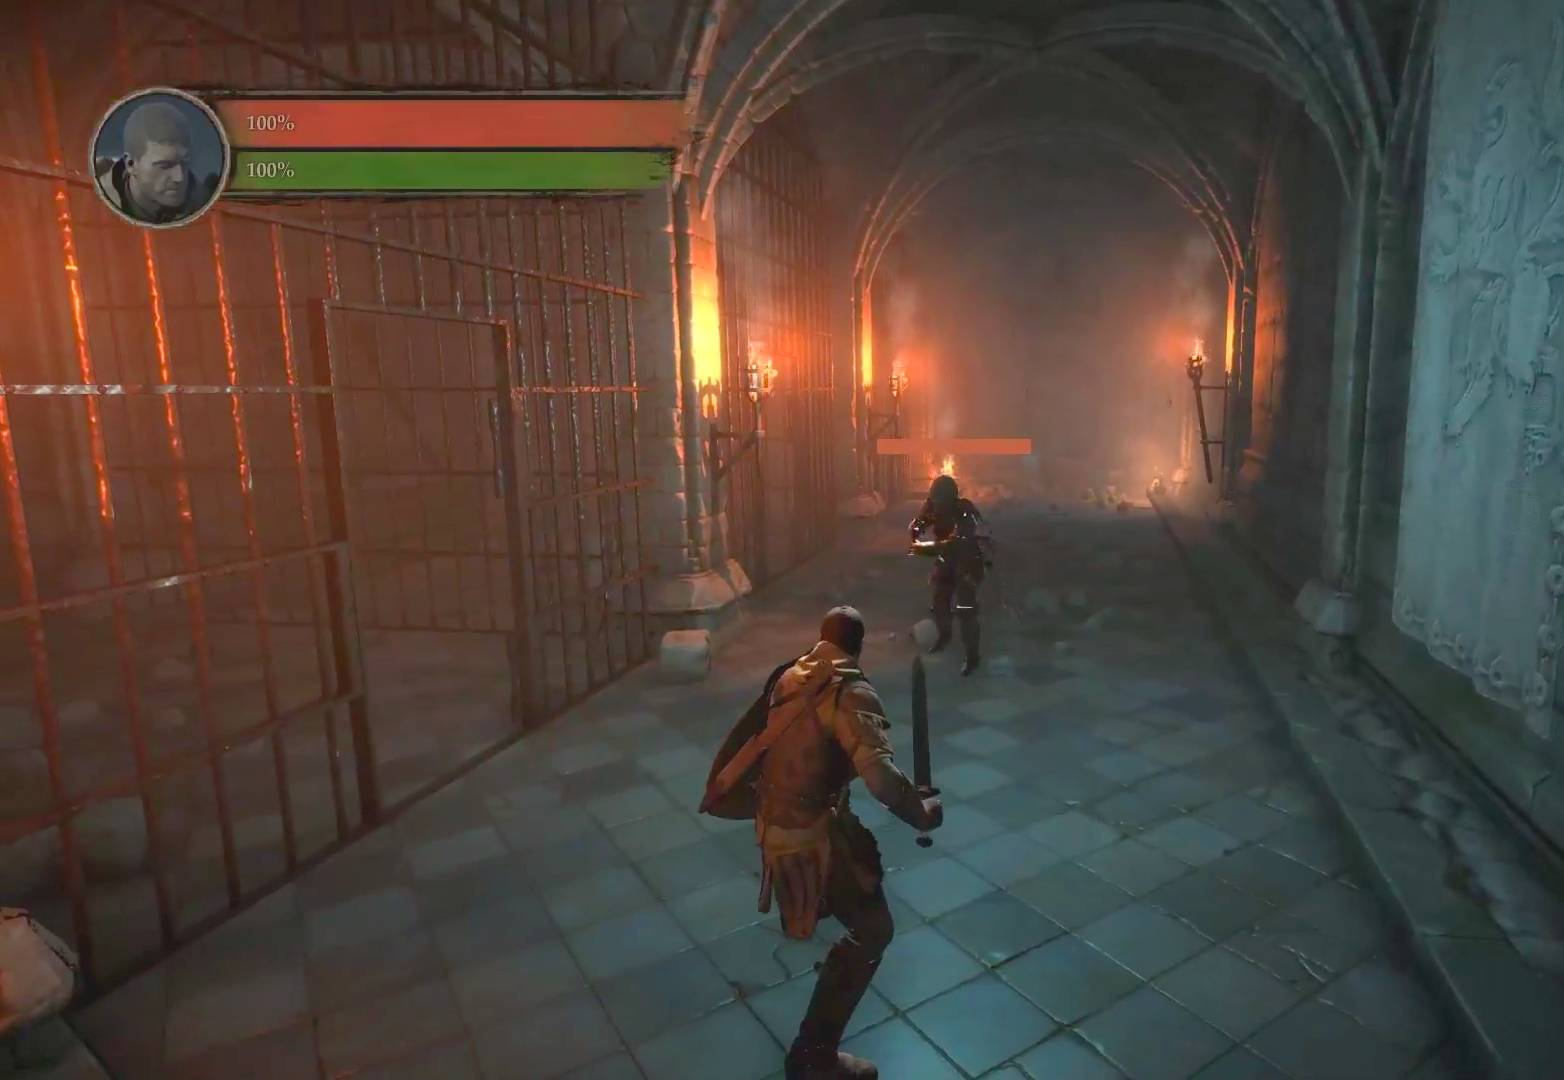
\includegraphics[width=26em]{figures/fig-bright-souls.jpg}
    \end{center}
    \legend{Source: Screen capture performed by the authors on a Microsoft Windows system.}
    \label{fig:ex1}
\end{figure}

To replicate the scenario of a successful commercial game, we look at how the problem of adaptive difficulty  is handled in multiple commercial games. Then, we analyze in depth the aspects that contribute to the difficulty of \emph{Dark Souls}, and attempt to replicate them in a simplified implementation. We compare the implementation of our solution to the original game, and outline the gameplay features that constitute the \emph{Souls}-like experience.

We propose a possible method for the design, implementation and usage of AGT as means of enhancing player experience. We compare the results in presence and absence of AGT, using as parameter a user evaluation on their perceived experience for each scenario and performance analysis based on gameplay data.

%============================================================

\chapter{RELATED WORK}
\label{ch:related-work}

\sepfootnotecontent{fn:speedrun-com-re4-guides}{Footnote: Speedrun.com Resident Evil 4 Guides}

\sepfootnotecontent{fn:beat-em-up}{Footnote: What are beat 'em up games}

In this chapter, we perform a review of previous research and literature related to adaptive systems and dynamic difficulty. We begin by reviewing literature regarding player experience and the concepts that define game difficulty to understand the impact of difficulty in player experience. We attempt to understand how difficulty can be detrimental or a support tool for players to learn, understand and improve upon the use of game mechanics and systems. We identify the problems with fixed difficulty curves, where the game provides a limited set of options for players to define their expected challenge level within the experience of a game. 

We proceed by studying some of the previous solutions that were develop to address the issue of player skill that is not properly represented by a limited set of difficulty curves and challenge levels. First, we understand the concept of player models, where player behavior is monitored and used as a tool to identify game design issues and improvements that directly affect player engagement. We compare that to the recent increase in research towards game analytics, where data from large user bases is aggregated to identify trends, problems and improvement opportunities in regards to game design.

We review some of the pioneering research on AGS (Adaptive Game Systems) \cite{ARTICLE_PlayerCentredGameDesign}, the category of solutions that propose to enhance user experience based on player profile and preferences. We attempt to understand how AGS can be used to alleviate the steep learning curve of highly challenging games, accommodating the skill level of beginner players to the level of challenge proposed by game developers in challenging video games. We review multiple dynamic difficulty implementation methods, such as \emph{probability-based}, \emph{affect-based} and \emph{learning-based} adjustments. We identify the problems with such methods in regards to how these methods can be adapted to commercial solutions, where changes, short deadlines and fast iterations are prevalent.

We also evaluate some of the efforts in adaptivity in commercial games, analyzing their positive and negative effects. We attempt to understand the impact of solutions implemented in some of the most successful commercial games in the last decades, specifying how the discovery of such adaptive systems affected the way that players form strategies and execute actions in such games. We attempt to identify some of the most representative examples in each dynamic adaptation category, and verify the shortcomings of each adaptation method.

% ================================================================================
% ================================================================================
% PLAYER EXPERIENCE AND DIFFICULTY
% ================================================================================
% ================================================================================

\section{Research on Player Experience and Difficulty}

The objective of this work is to create a reliable system that is able to improve experience for any player, regardless of their skill level and expected challenge towards a game. To understand how to improve player experience, we must first define what constitutes it. In this section, we identify the components that constitute player experience based on previous research in usability applied to the specific context of games. 

We attempt to extract concrete, functional features from the subjective term \emph{experience}, and translate these features into tools to design a proper challenge for the player, as well as to avoid mistakes and misconceptions on level design. To perform such a task, we analyze the impact of difficulty in games and its boundaries by reviewing literature on the psychology of player enjoyment. We review why the correct level of challenge can contribute to increasing levels of immersion and the overall positive experience of a player.

\subsection{Definition of Player Experience}

Computer software is commonly developed with the objective of allowing an user to execute a set of tasks, determined by a clear objective and in a specific context \cite{ARTICLE_FromUsabilityToPlayability}. One of the early endeavors in the field of HCI (Human-Computer Interaction) was the efficiency of performing the \emph{task} to ensure a product's instrumental value \cite{ARTICLE_UserExperienceAResearchAgenda}. In this line of thought, users of an application should ideally perform tasks without thinking about the application. 

Research on the interaction between people and systems in the field of HCI led to the concept of \emph{usability}, defined by \cite{ISO_ISO92411} as:

\begin{quotation}
"The extent to which a system, product or service can be used by specified users to achieve specified goals with effectiveness, efficiency and satisfaction in a specified context of use."
\end{quotation}

This definition specifies the three qualities of a usable product: \emph{effectiveness}, \emph{efficiency} and \emph{satisfaction}. We argue that while effectiveness and efficiency can be related to productivity,  satisfaction may not be fulfilled solely by productivity. For instance, an user might feel dissatisfied with the audiovisual components of an application such as its interface, even though the application perfectly satisfies the purpose of assisting in the completion of tasks efficiently.

In \citep{ARTICLE_UserExperienceAResearchAgenda}, we learn that early works on usability expressed that productivity is not primary, but only a contributor to \emph{User Experience}. The term "user experience" does not have a standard definition, but can be seen as how people interact with products and the resulting experience and emotions \cite{ARTICLE_UnderstandingExperience}. The experience is therefore a consequence of: the user's state, such as their emotions and needs; the characteristics of the product, such as usability and audiovisual aspects and the context of use, such as the environment and date.

According to \cite{ARTICLE_FromUsabilityToPlayability}, the concept of \emph{usability} is not sufficient to fully describe UX (User Experience) in relation to Video Games. The authors argue that video games are a specific type of interactive system used for leisure purposes. Thus, when evaluating quality not only instrumental values should be considered, but also non-instrumental values such as storytelling, visuals and character design. The author also introduces the concept of \emph{Player Experience}, a specialization of UX that emphasizes the specific properties of experience in games.

The author explains that Player Experience is characterized by \emph{Playability}, a concept based on Usability but with different meanings in the video game context. The proposed definition of \emph{Playability} by \cite{ARTICLE_FromUsabilityToPlayability} resembles the original Usability definition, but emphasizes the user-centric perspective and the satisfaction property:

\begin{quotation}
"Playability represents the degree to which specified users can achieve specified goals with effectiveness, efficiency and specially satisfaction and fun in a playable context of use."
\end{quotation}

This definition is further explained when the author introduces a set of seven attributes that compose Playability: \emph{Satisfaction}, \emph{Learnability}, \emph{Effectiveness}, \emph{Immersion}, \emph{Motivation}, \emph{Emotion} and \emph{Socialization}. The concepts of effectiveness and satisfaction remain present in this definition, but are specialized or complemented. Efficiency is specified as \emph{learnability} and \emph{immersion}, and the satisfaction aspect is complemented by\emph{emotion}, \emph{motivation} and \emph{socialization} to define a set of user-centred attributes. Since this work focuses on a single-player environment, we will discuss the first six attributes and evaluate which of them can be manipulated by a reliable system through AGT.

\emph{Satisfaction} is the degree of enjoyment derived from playing, characterized by \emph{fun}, \emph{disappointment} and \emph{attractiveness}. Fun is classified as the ability of a game to entertain the player whether through challenge, curiosity or competition. Disappointment refers to the feeling of disappointment of the player in relation to a game. Attractiveness encompasses any functional or aesthetic features that increases the pleasure of play such as realistic visuals, exceptional character design or interesting systems.

\emph{Learnability} is defined as the player's capacity to understand the game systems and improve their level of proficiency in relation to the game. It is categorized by \emph{Game Knowledge}, \emph{Difficulty}, \emph{Frustration}, \emph{Speed} and \emph{Discovery}. In this context, Game Knowledge refers to the player's prior expertise to the game's mechanics and environment, and influences how the player is affected by the \emph{learning curve} [FN]. Skill can be identified in the player's cognitive aspects such as strategic and analytic decision-making, or interactive aspects with efficient usage of game mechanics.

\emph{Difficulty} relates to the challenge perceived by a player in relation to their skill. The degree of difficulty can either encourage a player to improve by learning how to play or cause frustration. Frustration relates to the feeling of uneasiness when failing to complete a particular objective and is often part of the learning process. Speed refers to the pace in which new concepts are presented to players and affects the game's learning curve. Discovery refers to the techniques employed by the game to help players assimilate game content such as interfaces or level design, and directly affects the learning curve.

\emph{Effectiveness} refers to the resources necessary to entertain players, determined by \emph{Completion} and \emph{Structuring}. Completion is related to the overall percentage of players that feel motivated to reach the game's final goal. Structuring emphasizes the locality of content as when, where and how gameplay elements appear in the game. For instance, the placement of enemies and level geometry will contribute to how the player perceives and performs an objective, indirectly affecting the learning process.

\emph{Immersion} depicts the capacity of a game to be believable in a way that the player becomes involved, losing their awareness of surroundings and sense of time. The \emph{immersion} factor can be determined by \emph{Conscious Awareness}, \emph{Absorption}, \emph{Realism} and \emph{Dexterity}. Conscious Awareness is the degree to which a player is aware of the in-game outcomes of their actions, so that they can effectively plan and execute according to a situation. Absorption refers to the level of focus of a player has to a game in a given moment, and is inversely proportional to the level of focus to their real world surroundings. Realism depicts how the game's presentation influences the ease of player absorption, relying in game characteristics such as controls and game atmosphere. Dexterity relates to the ease of a player handling the game's controls and systems, so that performing in-game actions is natural and effortless.

\emph{Motivation} is the group of attributes that compel the player to perform one or various in-game actions, defined by \emph{Encouragement}, \emph{Curiosity} and \emph{Self-Improvement}. Encouragement is the level of confidence felt by a player when facing unexplored challenges. Curiosity is the degree to which a player is interested in interacting with new elements. Self-Improvement is the process of ability development and happens any time a player must overcome a challenge that is more difficult than their skill level. 

\emph{Emotion} refers to involuntary player responses to the cognitive stimulus of a video game, defined by \emph{Reaction}, \emph{Conduct} and \emph{Sensory Appeal}. Reaction consists of the emotional response of a player in relation to a series of in-game events. Conduct is the ability of a game to conduct a player through a proposed range of emotions caused by different stimuli. Sensory Appeal denotes how interesting a game is in the aesthetic perspective using different sensory channels. For instance, a game with realistic graphics and sound effects might appeal to the audiovisual sensory channel of players.

The definition of \emph{Playability} proposed by \citet{ARTICLE_FromUsabilityToPlayability} defined several attributes that categorize the characteristics of a player, the resources employed by a game and how different game aspects are able to affect a player. We argue that one of the concepts that is most frequently discussed in this work is that of  \emph{Challenge}. If challenge is presented poorly, the player might feel frustrated and discouraged to self-improve. Thus, the level of challenge must not deviate exceedingly from the level of skill by a player. In another perspective, challenge by itself can be a motivating factor for self-improvement and contribute to the overall satisfaction.  

Challenge is defined by the difficulty of an objective, the overall learning curve and player skill level. Therefore, it is directly related to how well a player learns and adapts to the game's systems. Therefore, it is imperative to comprehend how challenge fully affects players, and how learning tools such as \emph{Failure} and \emph{Punishment} are employed in game systems.

\subsection{Challenge and Flow in Games}
\label{sec:challenge-flow}

Failure can be described when a player is unsuccessful in the completion of an in-game task. In the event of failure, video games punish the player with some type of progression loss or setback. In the classic Arcade-style game \emph{Tetris}, the player must replay the game from the beginning upon losing. While this approach might be acceptable in session-oriented games with no narrative progress, modern Game Design encourages the usage of less punishing setbacks such as restarting at \emph{checkpoints}.

The perceptible change in failure outcomes suggests that punishment could be detrimental on the enjoyment of a game, depending on its gravity. The controversy of player failure and punishment requires the clarification of its purpose in games. If the only possible outcome of losing was a negative experience, the very existence of this system would be questionable.

According to \cite{ARTICLE_FearOfFailure}, failure serves the function of making players readjust their perception of a game. When a player fails performing a task, they realize the strategy that was performed is not the correct or optimal solution to a problem. The player then reevaluates the situation, analyzes what caused the failure and attempts a new strategy. This cycle provides the player an opportunity to deepen their knowledge, and encourages the creativity of new solutions.

We argue that punishment in games serves the purpose of establishing the contrast between consequences of player actions. In a simple perspective, punishment explains the rules of a game, and how a player is supposed to play it. In the game \emph{Super Mario Bros} (1985), the player has a predetermined number of lives upon starting the game, which is decreased with each death. Upon dying, the player is punished by replaying the current level. If all lives are lost, the player replays the entire game from the beginning.

The aversion to losing the progress made in a game serves as encouragement for the player to learn how to avoid defeat. In \emph{Super Mario Bros}, the player quickly learns that enemies should be avoided or beaten, and lava or bottomless pits should be evaded. If punishment mechanics did not exist, the player would simply progress by running to the right until reaching the end of a level without taking part in the proposed gameplay mechanics.

In the case of Dark Souls, punishment is used as a tool to create tension and increase player awareness. With each death, the player loses all their experience points\footnote{Experience Points are resources acquired by the player upon defeating enemies with the purpose of serving as a currency for purchasing upgrades for the player character. Such upgrades can improve the efficiency of the player in combat, or enable the player to use better equipment. In the Dark Souls game series, the Experience Points, also known as "Souls", can also be used for trading with \emph{NPCs} (Non-Player Characters) for purchasing various items which assist the player when progressing.}. If a player wishes to recover them, they must retrieve them from the same position where they were defeated. Dying again means the experience points are lost permanently. In other words, the player is forced to beat the challenges they previously failed to avoid progression loss. Death in Dark Souls can be an extremely frustrating experience, and arguably be considered as overly punishing.

Since the experience points are used to evolve the character and directly affect the outcome of future encounters, the player is encouraged to survive by any means after accumulating a reasonable amount. Upon reaching a checkpoint, the player can then spend their experience points to attain permanent attribute bonuses. Therefore, the fear of losing character progress before reaching a checkpoint reinforces the necessity of careful and strategical decision making.

While the philosophy of punishment as a tool is powerful as means of encouraging learning and adaptation, it can also be the source of anxiety and demotivation. If the punishment mechanics do not provide possibility of player evolution, they aggravate the exhaustion of repeatedly trying without success. We argue that if a game is excessively challenging to the skill level of a player, overly punishing will be the catalyst to surrender. Thus, the game system should also take in account the levels of punishment required to encourage player evolution without hindering the learning process.

In the context of video games, challenge is an abstract concept commonly referred as the player's perception of difficulty \cite{ARTICLE_RoleOfChallenge}. If a game is considered challenging by the general public, the majority of players would agree that the game requires a high skill level to complete. Nonetheless, a game that is considered easy by the public can still be challenging to a smaller audience with less technique or experience.

The difference between the level of challenge and skill directly affects the quality of player experience. If a game is too easy to the skill level of a player, they will not feel any sense of accomplishment upon completion and will experience boredom. If a game is too hard, the player might feel overwhelmed and experience anxiety. This is supported by the Theory of Flow, proposed by \cite{BOOK_Flow}.

The Theory of Flow indicates the existence of a state of complete focus in an activity, with a high level of energy, enjoyment and fulfillment. In this state, people lose track of time and external problems. Flow is considered to be state where optimal experience takes place. The level of focus achieved in being such a state maximizes the pleasure and performance of an activity.

According to the Theory of Flow, the main components of Flow are a challenging activity, the merging of action and awareness, clear goals, immediate feedback, concentration, a sense of control, loss of self-consciousness and an altered sense of time. However, not all of them are needed for an activity to provide the user the feeling of Flow. These descriptions of Flow can be observed in games when a player becomes immersed, temporarily engaging the perspective of a virtual reality.

The Theory of Flow also states that to maintain the state of Flow, the challenge of an activity must be balanced to the abilities of the person performing it. This concept is known as \emph{Flow Channel} or \emph{Flow Zone}. This can be translated directly to the concepts of Difficulty and player Skill Level in gaming. Different players will present different Flow Channels. Hardcore players will prefer more aggressive challenge scaling in comparison to their skill, whereas Casual or Novice players will prefer a more subtle introduction to the game's complexity \cite{ARTICLE_FlowInGames}. Figure \ref{fig:flow-channel} exemplifies the \emph{Flow Channel}, where a balance of difficulty and player skill denotes the optimal conditions for player immersion and focus.

\begin{figure}
    \caption{A visual representation of the concept of \emph{Flow Channel} or \emph{Flow Zone} discussed in \cite{BOOK_Flow}.}
    \begin{center}
        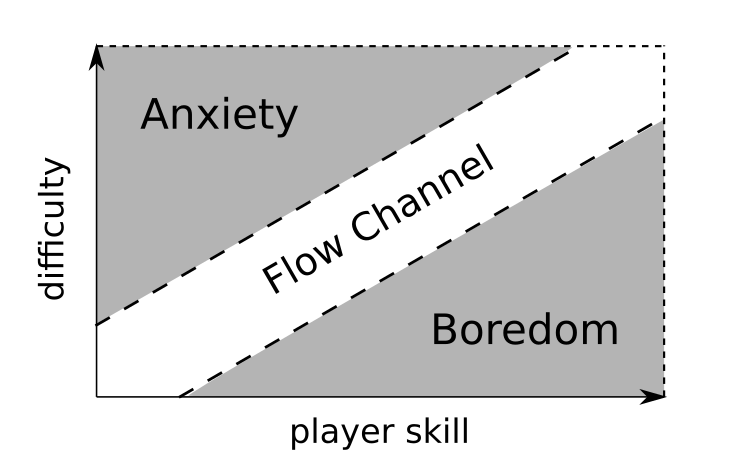
\includegraphics[width=26em]{figures/fig-flow-channel.png}
    \end{center}
    \legend{Source: Diagram assembled by the authors based on the concepts defined by \cite{BOOK_Flow}.}
    \label{fig:flow-channel}
\end{figure}

The balance between challenge and skill strongly contributes to the optimal experience of a player, and is referred to as a defining factor on the quality of a game \cite{ARTICLE_FearOfFailure}. We argue that we can balance the level of challenge through AGT. By acquiring information on the profile and preferences of a player, we can either ramp up the difficulty or encourage the learning process. Therefore, we understand that the usage of AGT can directly contribute to a positive experience.

\subsection{Learning Curve}
\label{sec:learning-curve}

Another interesting concept in games is the \emph{learning curve} \cite{article_learningcurve}. The learning curve depicts how easy it is to become used to the game's mechanics and systems. Game Developers often consider the learning curve as a key reference when performing level design. The first few levels of a game should enable the player to learn each mechanic in an isolated and controlled environment, whereas the last levels of a game should be designed considering that the player has knowledge about all the mechanics proposed by the game designer, and thus should present challenges that require mastery of each mechanic to surpass. Figure \ref{fig:difficulty-curves} depicts multiple possibilities for difficulty curves as a function of player progress in a game.

\begin{figure}
    \caption{Examples of the distribution of difficulty in games as a function of player progress.}
    \begin{center}
        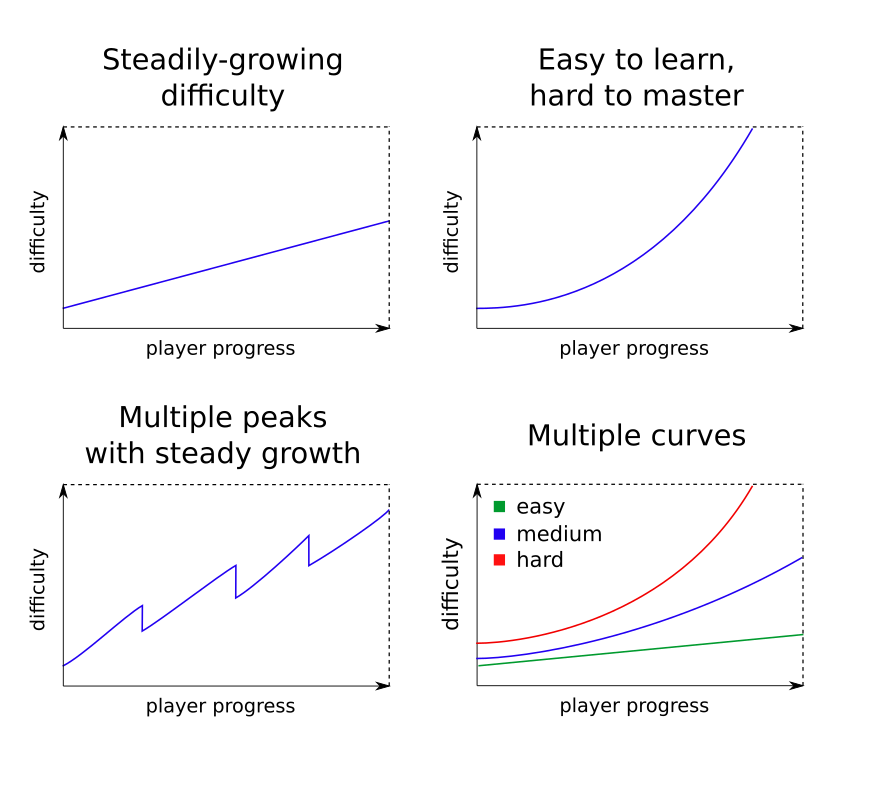
\includegraphics[width=26em]{figures/fig-difficulty-curves.png}
    \end{center}
    \legend{Source: Diagram assembled by the authors.}
    \label{fig:difficulty-curves}
\end{figure}

Perhaps the most notable example in teaching game mechanics through a concise learning curve is seen the famous game \emph{Super Mario Bros} \footnote{Super Mario Bros (Nintendo, 1985). Video Game. Nintendo Entertainment System.} in World 1-1, as addressed in \cite{video_extracreditsmario11}. In the first thirty seconds of gameplay, the player is able to learn that they must progress going to the right, that enemies must be avoided or eliminated by jumping in their heads and that special blocks hide valuable rewards such as additional lives. All the mechanics are taught without a single line of text or on-screen dialog box. Instead, the game teaches them by simply using the player's curiosity with an ingenious placement of game entities.

Some genres of games with consolidated and well-known mechanics share multiple similarities. The mechanics in such genres are proven to be one of the core constituents in their type of gameplay, and are expected by any non-novice player. One example would be the FPS (First Person Shooter) mechanics of \emph{Call of Duty: Modern Warfare}\footnote{Call of Duty: Modern Warfare (Infinity Ward, 2007). Computer Game. Microsoft Windows.}. The running, sprinting, strafing, vaulting, proning and iron-sighting mechanics were so exceptionally well done that they still remain in the most recent title of the series, \emph{Call of Duty: Black Ops 4}\footnote{Call of Duty: Black Ops 4 (Treyarch, 2018). Computer Game. Microsoft Windows.}. Other entries in the FPS genre such as \emph{Battlefield}\footnote{Battlefield 5 (DICE, 2018). Computer Game. Microsoft Windows.} also employ the same set of mechanics, which has since then become almost a requirement for the non-tactical Arcade Shooter style.

Arguably, games with the mechanics of a consolidated genre have a faster initial learning curve to any player that has played a similar game before. These games take advantage of that, and throw the player straight into the action. Within the first few minutes of playing a \emph{Call of Duty} game, the player will have faced and beaten an impressive amount of enemies. They will also confirm their proficiency by choosing exactly the difficulty level that appeals to their skill. Therefore, the veteran player of such a genre knows what to expect of the game and its standard difficulty level. They tailor their game experience to the optimal experience in the act of leisure.

We argue that Adaptive Game Technologies can also have an impact on the learning curve issue. Understanding the profile of a player before gameplay takes place can be a key factor on the decision to ramp up the initial challenge of a game, and remove or alter initial sections which only serve the purpose of teaching basic mechanics.

Thus, the learning curve should not be static, but customized to the needs of each player. If the player has already mastered the base concepts of a game, they should be encouraged to using their knowledge to the fullest. Tailoring the learning experience to each player could balance the challenges faced by the player to a more appropriate, which could possibly increase the sense of enjoyment and immersion as seen in \autoref{sec:challenge-flow}.

% ================================================================================
% ================================================================================
% ADAPTIVITY IN RESEARCH
% ================================================================================
% ================================================================================

\section{Adaptive Systems In Research}

Mechanisms for DDA should describe what elements of the game are going to be monitored, and what variables should be adjusted accordingly. Therefore, the functionality of a DDA system can be summarized as a relation between observation and adjustment. Since video games are so diverse in design and functionality, the mapping between observation parameters and adjustment variables has yet not been efficiently described as an universal and generic approach \cite{PHD_DynamicDifficultyAdjustment}. Rather, the game developer should decide what variables should be observed and adjusted in a per-game basis.

In contrast to the implementations of DDA portrayed in commercial games, prior academic work encompassed a multitude of probabilistic models and data-driven approaches that could prove to be interesting if applied to a commercial solution. In the scope of this work, we use the literary review in \cite{article_ddareview} as a reference to categorize a subset of DDA algorithm variants implemented in previous academic work, as well as to select and perform an analysis on a single relevant representation for each of the proposed solutions.

% =======================================================
% PLAYER MODELING
% =======================================================

\subsection{Player Modeling and Profiling}

The concept of adaptivity in games relates to how a game is able to adapt its content based on the \emph{profile} and \emph{preferences} of a player, which constitute \emph{player models} obtained from a multitude of \emph{Player Modeling} techniques. Player Modeling allows the creation, collection and processing of \emph{player models}, real-time collected data sets that can be classified into reality-based player types \cite{ARTICLE_DynamicPlayerModelling}. Knowledge about player types allows dynamic adjustment in the sense of content customization, where a game designer might dynamically assign what should be presented to each type of player.

In a DDA system, \emph{Player Models} refer to collections of data gathered to be used as a metric for adjustment policies \cite{PHD_DynamicDifficultyAdjustment}. Player Model data might be gathered during a play session as a trace of the player's actions and events in a game, or as static data collected from surveys or through the use of a gaming platform such as \emph{Steam}.

One possible implementation of a \emph{Player Model} consists of defining a collection of numerical attributes that describe the playing style of an individual player, as seen in \cite{BOOK_PlayerModeling}. Each attribute defines an aspect of the player's behavior, which is generally associated with their strategy or mechanical skill. A typical example of Player Model in a Shooter game can be seen in Listing \ref{lst:PlayerModellingExample}.

\begin{lstlisting}[caption={Example of a Player Model for a shooter game.},label={lst:PlayerModellingExample}]
class PlayerModel {
  public:
    enum Attribute {
      bCanStrafe,
      bCanFlick,
      bDoesStationaryShooting,
      fPrecision,
      fEncounterDuration,
      fKillsPerRound,
      fDamagePerRound,
      fDistancePerRound
    }
    void Initialize();
    void UpdateAttribute(Attribute att, float newValue);
    float GetAttribute(Attribute att);
    private:
      vector<float> attributeValues;
};
\end{lstlisting}

The values for each attribute are unknown to the game preceding a session. Therefore, it is necessary to sample and adjust the values during gameplay. Each time a sample is collected, the Player Model should reflect a player's behavior with increasing precision. In the implementation proposed by \citet{BOOK_PlayerModeling}, the attribute update function uses the \emph{Least Mean Squares} (LMS) training rule, commonly used in machine learning:

\begin{lstlisting}[caption={Implementation of attribute update using least mean squares.},label={lst:AttributeUpdate}]
float UpdateAttribute(Attribute att, float value) {
    float currvalue = attributeValues[att]; N
    float delta = value - currvalue;
    float weightedDelta = LEARNING_RATE * delta;
    attributeValues[att] += weightedDelta;
}
\end{lstlisting}

Attributes in this implementation consist of values between 0 and 1, indicating the probability of a player performing an action. In Listing \ref{lst:PlayerModellingExample}, this can be seen in the definitions of Boolean attributes (prefix 'b'). However, it is also possible to use the same approach to approximate statistical values, such as the damage a player inflicts per round. The value for each attribute represents the game's current best guess. Each sample collected contributes to the estimate weighted by LEARNING\_RATE. Therefore, for lower LEARNING\_RATE values more samples are required to sufficiently approximate an attribute. In most cases, values between 0.1 and 0.3 are used \cite{BOOK_PlayerModeling}.

Another perspective brought to the concept of player models is seen in \cite{ARTICLE_DynamicPlayerModelling}, where the authors describe a Player Modeling framework that takes \emph{concept drift} into consideration, which is the possibility of players adapting or changing behaviors and play styles according to their evolution or progress in a game. The framework relies on two sources of player-related data: information of player preferences inputted by a player prior to application use and tracking player performance in-game. Figure \ref{fig:dynamic-player-model} exemplifies the dynamic player model framework.

The discussion in \cite{ARTICLE_DynamicPlayerModelling} emphasizes the necessity of remodeling player types after measuring the effectiveness of adaptation. This means that a DDA system should be able to gather some type of player feedback regarding the effectiveness of the dynamic adjustments that were performed during play, and recreate the player profile based on this feedback. Some methods for gathering such feedback include inferring the player's affective state, such as with physiological sensors or from a camera or an analysis of statistical data retrieved from in-game attributes, such as player performance or their action history.

\begin{figure}[!ht]
    \caption{A representation of the dynamic player modeling framework discussed in \cite{ARTICLE_DynamicPlayerModelling}.}
    \begin{center}
        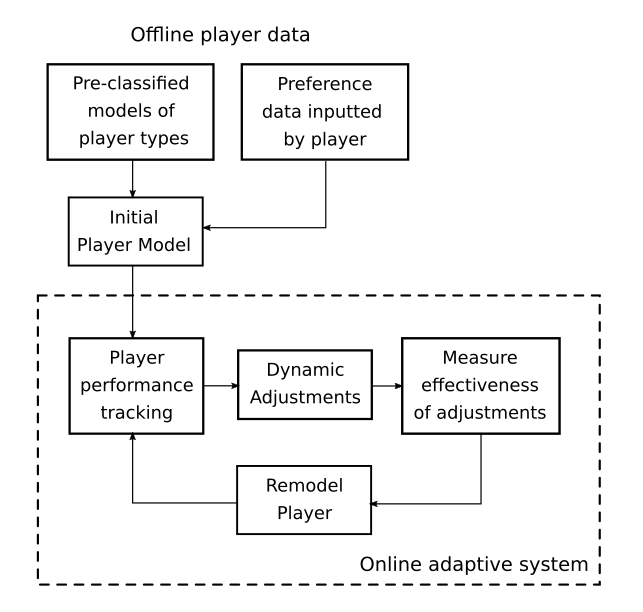
\includegraphics[width=26em]{figures/fig-dynamic-player-model.png}
    \end{center}
    \legend{Source: Diagram assembled by the authors based on visual representations in \cite{ARTICLE_DynamicPlayerModelling}.}
    \label{fig:dynamic-player-model}
\end{figure}

% =======================================================
% PROBABILISTIC DDA
% =======================================================

\subsection{Probabilistic DDA Systems}
\label{sec:statistical-adjustments}

One of the first and most relevant implementations of the probabilistic model approach for DDA systems is the Hamlet system seen in \cite{article_casefordynamicdifficulty}. Hamlet is a probability-based predictive system that is able to perform reactive and proactive adjustments to the distribution of items throughout levels of customized Half-Life \footnote{Half-Life (Valve Software, 1998). Computer Game. Microsoft Windows.} map \cite{article_casefordynamicdifficulty}. The system works by defining a finite set of possible game world states, and performing adjustments with the objective of avoiding game state "loops", where a player would perform the same set of actions repeatedly.

First, Hamlet establishes the probabilistic distribution of damage done to the player using a series of measurements taken over time. By doing this for each of the enemy classes, the probability of the player dying during an encounter can be estimated. Then, if the probability of death for an encounter is above 40\%, the system intervenes by distributing \emph{healing items}\footnote{Healing items in games are consumable resources that restore a percentage of the maximum health points of a player. An example for this are the health stations in the Half-Life franchise, where the player heals up to 80\% of their maximum health points upon interaction, but the resource is permanently depleted after use.} throughout the level before an encounter takes place. This is an example of \emph{proactive adjustment}, which occurs before an in-game event takes place. The author of the article argues that the effectiveness of proactive adjustments is harder to measure than \emph{reactive} adjustments, and thus this type of adjustment should be performed based on predefined constraints determined by the game designer.

Hamlet is also able to perform \emph{reactive} adjustments that occur during combat encounters, such as adjusting the maximum hit points for an enemy class or modifying the accuracy of enemy shots. The objective of any adjustment is to decrease the amount of player deaths for each level independently of player skill, and to achieve a mean health percentage of 60 with a standard deviation of 15 points at any given point.

Results of the experiment using the Hamlet system showed that most players were unable to recognize when the system was performing adjustments, or characteristics of the game were modified when adjustments were performed. Some players suggested that the system performed adjustments that were not there, and several players suggested that the system did not perform any adjustments based on their skill level. During the post evaluation interviews, there was a slight correlation between the adjustment policies and player enjoyment when considering players with expert skill level, although players with novice skill level did not report any perceivable change.

The study concluded that adjustment algorithms can include the performance of a player while retaining the player's sense of agency and control. When performed with accordance to the game's core design, adjustments can be nearly imperceptible, and slightly increase the sense of enjoyment of a player without diverging from the proposed experience.

Therefore, the Hamlet system proposed by \citet{article_casefordynamicdifficulty} addresses the possibility of predicting gameplay outcomes given a game world state, and performing \emph{reactive} or \emph{proactive} adjustments for a more immediate resolution when compared to other solutions. We argue that while this might be an interesting approach for a supportive or secondary DDA system, this type of solution might be hard to tailor from a game designer's perspective since it is impossible to predict results functionally.

% =======================================================
% AFFECT-BASED DDA
% =======================================================

\subsection{Affect-based DDA Systems}

Most implementations of DDA systems use as adjustment policies metrics that would represent player performance. However, the affective state experienced by players could also play a key role in the gaming experience, and thus could be a useful metric for adjustment policies in DDA systems. This is the theme of the work presented in \cite{article_affectivedda}, where physiological signals were tracked to infer the anxiety level of players, and then used as a metric to perform dynamic adjustments.

The work of \citet{article_affectivedda} cites previous research indicating that electrodermal and cardiovascular activities had a relation to anxiety levels. An increase in skin conductance may be caused by anxiety. A decrease of parasympathetic activity and increase in sympathetic activity in the heart also may suggest anxiety \cite{article_affectivedda}.

Blood pulse volume measured at fingers were also shown to be subject to stress manipulation, and presents a correlation with self-reported anxiety \cite{article_affectivedda}. Measures of EMG (Electromyography) activity of specific muscles (such as Corrugator Supercilii) were also shown to be strong indicators of anxiety.

Therefore, the work presented in \cite{article_affectivedda} used features of cardiovascular activity, such as interbeat interval, relative pulse volume, pulse transit time and heart sound; electrodermal activity (tonic and phasic response to skin conductance) and EMG activity (from Corrugator Supercilii, Zygomaticus and upper Trapezius muscles) as input measures to a Regression Tree (RT) technique which classifies the physiological signals into affective states that categorize anxiety levels.

A Pong-based game was implemented for the study, with two variations in difficulty adjustment algorithm: one where the difficulty would be adapted based on player performance (a relationship between points scored against or in favor of the player), and another where the anxiety level of the player is used as input to alter difficulty.

Three difficulty levels were implemented in total, which would be assigned depending on performance or anxiety levels: if the player's performance is classified as "Excellent", the player would progress into the next difficulty level. If the performance is classified as "Poor", the difficulty level would be decreased. The affect-based variant utilizes an analogue solution, where the difficulty is increased if the anxiety level is classified as "Low", and the difficulty is decreased if the anxiety level is classified as "High". Figure \ref{fig:affective-adaptation} displays state-flow diagrams representing the difficulty levels and their transition conditions.

\begin{figure}[!h]
    \caption{A state-flow diagram representation of the performance-based and anxiety-based adaptation variants in \cite{article_affectivedda}.}
    \begin{center}
        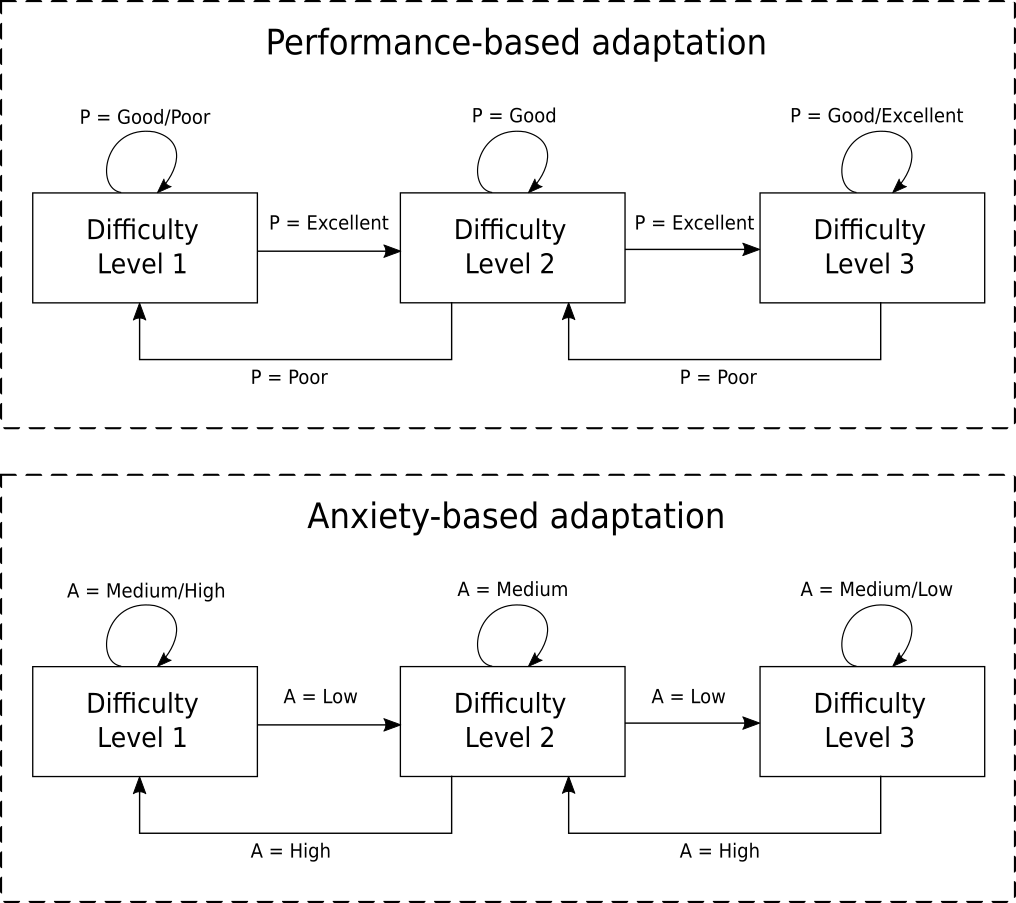
\includegraphics[width=26em]{figures/fig-affective-adaptation.png}
    \end{center}
    \legend{Source: Diagram assembled by the authors based on visual representations in \cite{article_affectivedda}.}
    \label{fig:affective-adaptation}
\end{figure}

The results of the experiment showed that the performance of most players improved during the affect-based DDA session in relation to the performance-based DDA session. Players also perceived the affect-based DDA version to be more challenging than performance-based DDA, and reported that the affective version was more satisfying.

We argue that, while the results of the experiment portrayed in \cite{article_affectivedda} showed mostly positive results in comparison to performance-tracking DDA, employing this type of solution in a commercial video game is not feasible, as current hardware is unable to track physiological signals in a significant way. 

Furthermore, the game implementation used for the experiment is a simplistic game with limited audiovisual feedback. Therefore, a similar experiment could be performed in a modern game with high audiovisual fidelity to evaluate results, as modern games are often able to evoke a multitude affective reactions by immersing the player in a \emph{cutscene}\footnote{A \emph{cutscene} is a special in-game event where the player is unable to input control into the game, and audiovisual feedback is a result of an automatic, predefined sequence of events determined by the game developers. Cutscenes can be seen as parts of a game that are similar to a movie, where the game is not interactive and instead focuses on telling a part of the story.} or a series of chaotic events.

% =======================================================
% LEARNING-BASED DDA
% =======================================================

\subsection{Reinforcement Learning in DDA Systems}

Another approach to adaptive difficulty involves the adaptation of AI (Artificial Intelligence) agent behaviors through reinforcement learning, as exemplified in \cite{article_adaptivebehaviorai}. Their implementation defines AI agents in a simple car simulation race game, where each player has the objective of passing through the maximum number of \emph{waypoints}\footnote{A \emph{waypoint} is a special position in a game world where an in-game event is toggled when the player is within interaction range. Waypoints are commonly used in games when the player has to take a specific path to a goal, with the game assigning several intermediary positions the player has to pass through to validate that the correct path was taken. In the context used for the implementation presented in \cite{article_adaptivebehaviorai}, waypoints are simply game world positions the cars must reach to score points. Each time one of these positions is occupied by a car, the waypoint is destroyed and a new random position is assigned elsewhere in the game world as the next waypoint.} in a given amount of time. Multiple waypoints are displayed on the screen at any given time, and a waypoint disappears when any of the players is within interaction range.

The AI agents implemented in \cite{article_adaptivebehaviorai} define two layers of behavioral AI components. The first layer contains components associated with driving functionality, with the objective of improving driving performance of the controller. The second layer is associated with tactical behavior components that seek to outplay the opponent in the game.

Driving behavior components ignore the existence of the opponent, leading to inferior performance in the game. Tactical behavior components help the AI controller decide which waypoint to head to, or if the controller should not head to a waypoint at all. In more general perspective, the Driving Behavior components can be seen as the mechanical input of AI agents in the game, whereas the Tactical Behavior components could be considered the high-level decision making components of the AI.

To evaluate the performance of adaptive AI agent controllers, two evolutionary computation algorithms are implemented: the adaptive uni-chromosome controller (AUC) and the adaptive duo-chromosome controller (ADC). The advantage of using such algorithms is that the training and adaptation process occurs in real time during the course of a game session.

Each chromosome in said algorithms stores seven real numbers representing the probability of activating a behavioral component whenever a waypoint is passed. Two metrics are used as an input for the adaptation algorithm: first, a minimization of the winning percentage difference (|W - L|, where W represents the wins and L represents the losses) and second, a minimization of the mean score difference (|s1-s2| where s1 and s2 represent the scores of player 1 and player 2).

To evaluate the efficiency of the proposed algorithms, the authors first compared the strongest AI agent that the adaptive system would possibly generate (defined by enabling all behavioral components simultaneously and permanently) against five static AI controllers based on various traits that would simulate various styles of play, such as heuristic controllers, reverse-enabled controllers, predictive fast controllers, and neural network controllers.

Sets of \emph{n = 5000} games were played for each opponent in each step of the experiment. Through the first step of the experiment, the authors validated that a fully-enabled adaptive AI controller (having all the behavioral components activated at all times) was a competent opponent with positive median score differences against all static AI controllers.

In the second step, the behaviors were activated randomly whenever a waypoint was crossed to demonstrate that an effective adaptation algorithm is necessary for different types of opponents. Results showed that the random behavior selection algorithm had negative median score differences against all five static controllers.

In the third step, the authors evaluate the use of the AUC algorithm. The expected behavior set encoded by a chromosome as a result of the algorithm should represent a "winning" strategy. Effects of varying \emph{Learning Rate} and \emph{Mutation Rate} were documented for the experiment, showing that the general trend of increasing learning rate is a gentle increase in the mean score difference, since a large learning rate quickly saturates chromosome values to either 0 or 1. Higher mutation rates tend to produce larger differences in mean score and winning percentage by producing large fluctuations in chromosome values. In general, high mutation rates led to poorer results, and the optimal value of 0.1 was stated for the AUC algorithm variant.

In the final step of the experiment, the use of the ADC algorithm is evaluated, with the same idea of varying the Learning and Mutation Rates. For the ADC algorithm, no trends were perceived in association with varying Learning rates. This would likely have been caused by the reduction of the frequency of update opportunities for each chromosome. In the ADC algorithm, only one of two chromosomes is updated each time a waypoint is passed. This means that on average each chromosome is updated half as frequently as chromosomes in the AUC variant. As for the Mutation rate, the results of the ADC controller improved greatly as mutation was introduced, possibly because the mutation operation offered more opportunities for the chromosome values to adapt.

As a conclusion to the experiment, the authors expressed that while the AUC algorithm had lower memory footprint, the ADC algorithm was able to better minimize the number of drawn games, which would possibly reduce player frustration. It was also noted that both the AUC and ADC algorithms were able to generate specific patterns of behavioral component distribution for each of the static controller stereotypes, meaning that the Reinforcement Learning technique would be able to adapt to different styles of play. The general intent of both algorithms was not to maximize the number of wins, but to maintain a fair and close challenge to the opponent by minimizing the score difference as well as the difference between number of wins and losses.

The work presented in \cite{article_adaptivebehaviorai} introduces the novelty approach of online learning without predefined data sets to the scenario of DDA solutions. It could be argued that the adjustment policies are also part of the reinforcement learning approach, since the decision of a behavioral component being activated or not relies on the algorithm being applied. This is an especially interesting solution since it lessens the responsibility of a game designer tailoring the boundaries of the adjustment system in advance of play. However, we argue that this experiment has yet to be applied in the context of real players using an implementation that would better replicate a commercial video game product.

% ================================================================================
% ================================================================================
% ADAPTIVITY IN COMMERCIAL GAMES
% ================================================================================
% ================================================================================

\section{Adaptive Systems In Commercial Games}

Several commercial games have attempted to create Dynamic Difficulty systems which embrace varying degrees of player skill, such as \emph{Mario Kart} \sepfootnote{fn:mario-kart}, \emph{Half-Life 2} \sepfootnote{fn:half-life-2}, \emph{Resident Evil 4} \sepfootnote{fn:resident-evil-4} and \emph{God Hand} \sepfootnote{fn:god-hand}. In this section, we look at examples of Adaptive Systems in some of the most popular games developed by the video game industry in the last decades. We categorize the solutions based on which game systems they affect, and discuss some of the caveats of each system.

% =======================================================
% RUBBER BANDING ADAPTIVITY
% =======================================================

\subsection{Rubber-banding in Mario Kart}

Perhaps the most popular approach to Adaptive Difficulty is found in games which present \emph{rubber banding}. This technique is most commonly seen in racing games that have artificial intelligence agents as opponents to the player. If the player performs exceptionally well in a race and is far ahead of every AI opponent, the opponents will receive a significant speed boost that often surpasses the standard speed limits of the game. In case the player performs poorly, the AI is slowed down below their base speed so that the player is able to catch up. The term \emph{rubber banding} derives from the analogy that the players and their opponents are held together by a rubber band, so that they are never too far apart from their opponents.

Rubber banding is employed to cause the impression that the outcome of the race is never clearly defined, enabling the perception that mistakes by the competitor that is ahead can greatly affect their chances of winning. The existence of the rubber banding system, along with the perception caused by it, results in the increase of tension and focus by the player. Rubber banding is not limited to the Racing games genre, and it does necessarily happen only between players and AI. However, it does imply that the game has some sort of competition system, even if the game is a single-player \footnote{A single player game is a video game where the input processed by the game is received from only one human user (player) during the course of a game session. All entities the player interacts within the game world are non-player entities.} or cooperative \footnote{Cooperative games are games in which the input is received from multiple human users (players), with each player controlling a different in-game entity. The players share a common objective, and must cooperate by combining their available commands and actions to achieve the winning condition.} experience.

Mario Kart applies rubber banding through two different methods, affecting both players and computer-controlled opponents \cite{website_rubberbandingmariokart}. The first type of rubber banding compares the performance of players to AI opponents: if a player is too far behind the computer-controlled opponents, the AI slows down by lowering their maximum speed. If a player is too far ahead, the AI receives a significant speed boost to their base speed. While being a simplistic solution common to many games in the racing genre, it attenuates the skill discrepancy between players and AI. 

The second solution in Mario Kart is presented through the power-up system, and targets the issue of skill discrepancy between players. Throughout the race, players are provided with multiple randomly-generated power-ups, which can be used to speed-up, attack or defend against opponents. Speed-up pickups are favored to players who are far behind others, whereas attack and defense power-ups are favored to players who are closer to attaining the first position. Players in the first position are generally provided the worse pickups. This provides better opportunities for players who are lower-skilled, as the access to speed power-ups is limited to the competitors who are far behind, and effectively serves as a catching-up mechanic.

While this solution is an interesting and creative effort that makes matches between players of varying skill levels more competitive, players that become aware of this system might avoid the first position to retain the best power-ups until the last moments of a race. This situation elicits the problem of meta-gaming in adaptive systems: when the adaptive systems are well-known by the users, exploits become a part of player strategy.

% =======================================================
% ENEMY BEHAVIOR & ITEM DISTRIBUTION ADAPTIVITY
% =======================================================

\subsection{Dynamic Items, Behaviors and Levels in Resident Evil 4}

\sepfootnotecontent{fn:re4-gameplay-description}{Footnote: What is Resident Evil 4 in terms of gameplay}

\sepfootnotecontent{fn:skill-ceiling}{Foonote: What is Skill Ceiling}

%   - In RE4 Level layouts, AI behavior and item distribution are affected by player performance 
Another interesting approach to adaptivity is seen in \emph{Resident Evil 4}\sepfootnote{fn:re4-gameplay-description}, where item distribution, AI behavior and enemy encounters are affected by different sets of information regarding player context and performance. Each system is affected by a different set of contextual metrics, and may enable or disable certain gameplay aspects independently based on the values presented by such metrics.

\subsubsection{Dynamic Item Distribution}

% ============================
% How the Dynamic Item Distribution System works
% ============================
%   - Dynamic Item Distribution Affects RNG systems by modifying loot tables based on player needs at a given context
%   - When player has low health, item distribution prioritizes health items
%   - If player has surplus ammo & health, prioritizes gold coins
%   - Veteran players control the use of resources 
The \emph{Dynamic Item distribution} System affects RNG (Random Number Generation) systems by modifying the chances of items being spawned when a player interacts with containers or defeats an enemy. The values that are modified depend on the current status and context of the player such as their health and the items in their inventory.

For instance, if the player has a low amount of health and no health recovery items in their inventory, the Dynamic Item Distribution system modifies the chances of health recovery items being distributed. If the player has a stabilized amount of health but lacks a specific ammunition type, the game prioritizes the distribution of such ammunition type for the player. If the player is not in a dangerous situation and has surplus ammunition, the game prioritizes gold coins, which can be used to purchase powerful weapons and weapon upgrades. 

% Benefits of Dynamic Item Distribution
% ============================

% - One of the most prevalent types of systems due to:
%   - Easy to implement, as it just modifies chances
%   - Easy to understand by game designers
%   - Ease of abstraction
%    - On a first playthrough, hard to perceive RNG
%    - On RNG systems, hard to tell what factors can influence the loot table
% - Can be integrated into the iterative game design process
% - Balancing values can be replicated throughout game sections 
In the landscape of commercial games as a whole, Dynamic Item Distribution Systems are one of the most prevalent types of adaptive systems employed due to:
\begin{itemize} 
    \item{Their ease of implementation, which involves monitoring of contextual values for player status and performance and simple modification of statistical values;}
    \item{Their straightforward process of adjustment, in which the values can be easily understood and tailored by game designers between playtests;}
    \item{The possibility to integrate them in the iterative nature of the game development process, where values can easily be adjusted between multiple play sessions;}
    \item{The fact that the balancement of item distribution can be replicated througout multiple sections of a game;}
    \item{The fact that they are abstract in nature, meaning that players have difficulty recognizing their existence or the complete extent of the modifications they perform.}
    \item{Their relation with RNG item distribution chance tables, where the factors that influence the chances for each element are ambiguous even for veteran players.}
\end{itemize}

% Examples of other successful games that use dynamic item distribution
%   - Half Life 2
%   - Left 4 Dead
%   - Diablo
Examples of other successful games that also use Dynamic Item Distribution Systems include \emph{Half-Life 2}, where resources are spawned in containers such as destructible boxes based on player health and ammunition; \emph{Left 4 Dead}, where the spawn points of weapons, ammunition and health kits are toggled in fixed spots based on how well the team is performing throughout a level; and \emph{Diablo}, where the rarity of items dropped by defeated enemies depends on the level, modifiers and rarity of the enemy.

% - Can help beginner players 
% - Highly skilled players are rewarded for their performance
In the specific case of Resident Evil 4, Dynamic Item Distribution may benefit beginner players by providing a steady supply of health and ammunition resources during sections of the game with intense combat encounters. The system always prioritizes the most important necessity for the player at a given moment, and as players are able to defeat enemies during a combat encounter, they are be supplied with ammunition and recovery items to be able to continue through a battle. For higher skilled players which are able to maintain a steady level of resources at their disposal, the game rewards performance with gold coins, which enables weapon upgrades that increase the efficiency at which the player is able to dispose of enemies. 

% Problems with Dynamic Item Distribution
% ============================

% - Beginner players could benefit from item hoarding
% - Important resources may not be distributed at critical sections of the game

% In harder sections of the game, beginner players generally need a high amount of resources due to the large amount of enemies being spawned and the lack of knowledge on how to deal with enemies
% As the player defeats enemies, loses health and spends ammunition, resources are constantly depleted from their inventory
Some of the problems involving the implementation of Dynamic Item Distribution in Resident Evil 4 can be analyzed through the perspective of beginner players when facing challenging sections of the game. In such sections, beginner players generally need to spend a higher amount of resources due to the large amount of enemies and their lack of knowledge on how to dispose of multiple enemies. As the player progresses through the combat encounter, they will likely lose significant amounts of health and ammunition. Therefore, resources will be constantly depleted from the player inventory, which is an expected result from the perspective of the Dynamic Distribution System. 

% At an initial point of a combat encounter, enemies would most likely drop less necessary resources such as gold coins
% Player may start to run out of resources at a critical point in the encounter, such when as when facing tougher enemies that are harder to dispose of
However, the main problem with resource distribution becomes evident when considering the flow of events in challenging combat encounters. Generally, at an initial point of the encounter the easiest enemies are spawned, and will most likely drop less necessary resources such as gold coins when defeated. After multiple waves of enemies the player may start to run out of resources, and at the same time progresses closer to the critical points in the encounter, such as facing special enemies that are harder to dispose of.

Since resource distribution is limited to the events of destroying containers and defeating enemies, beginner players that are unaware of the resource distribution system might destroy all containers at the beginning of an encounter, which causes the only resource distribution source to be the defeated enemies. At that point, tougher enemies which cause the player to generally lose more health and spend more ammunition might drain the player of all their resources before they are defeated.

% In conclusion, beginner players could benefit from the possibility of item hoarding for such encounters, which is harder to achieve due to the way dynamic item distribution is implemented
In such situations, a beginner player would benefit from the ability to perform \emph{item hoarding}, where the player accumulates resources over easier sections of a game to be spent on the more challenging levels. Because of the way item distribution is implemented in Resident Evil 4, item hoarding becomes harder to perform, since as the player accumulates health or ammunition resources the game will prioritize low necessity items such as gold coins.

% - Players may choose to not loot resource items purposefully
%   - Force the system to generate resource items only at critical sections of the game
%       - Maximize inventory space for weapons
%       - Maximize the money gained for upgrades
Additionally, a player that is aware of an adaptive distribution system might exploit the game by choosing to not loot items purposefully. By maintaining their resources at a controlled level, veteran players can prioritize the use of their inventories for important weapons and items, and force the system to distribute important resources at critical points in the game such as before an encounter with a large group of enemies. However, it can be argued that this characteristic can also be a benefit to highly skilled players, where good management of resources throughout the game can lead to rewards in terms of combat performance, as the player will possess better weapons and upgrades at their disposal.

\subsubsection{Dynamic AI Behaviors}

% ============================
% How the Dynamic AI Behavior System works
% ============================

%    - Affects the actions performed by AI agents
%    - Based on player performance and habits
The \emph{Dynamic AI Behaviors} system affects the actions performed by AI-controlled entities based on player performance and habits. In Resident Evil 4, players are able to increase their damage output and cause enemies to become staggered and unable to attack by shooting at their heads. When staggered, the player can also perform a \emph{kick attack}, which causes enemies to fall into the ground for a significant amount of time. 

%    - If player constantly headshots, enemies start to dodge, defend head & equip armor
If a player is constantly able to defeat enemies easily by shooting their heads or without spending significant resources such as ammunition and health recovery items, enemies will start to perform new actions such as attempting to dodge or even using their hands to block bullets. Additionally, enemies in later stages of the game will also equip protective apparel such as helmets and shields depending on player accuracy, which hinders the ability of the player to deal damage and cause staggers.

% - Experienced player can still be effective even with AI changes
Although the new actions and equipment presented by enemies can become an obstacle for effectiveness, they are not overwhelmingly difficult to handle. An experienced player can still be effective and shoot enemy heads with precision if they are able to predict enemy movement, react to character animations and use the proper weapons for each equipment.

% Benefits of Dynamic AI Behaviors
% ============================

% - Instead of making game super difficult, focuses on increasing skill ceiling
Therefore, instead of simply increasing the difficulty to an overwhelmingly high level of challenge, the implementation of Dynamic AI Behavior System in Resident Evil 4 causes the game to increase its skill ceiling\sepfootnote{fn:skill-ceiling} in an interesting way, enabling interesting situations in enemy encounters that can provide variety and challenge for experienced and highly skilled players.

% - The new actions performed by enemies are in-world elements that contribute to the believability of enemy behaviors, giving the sense that they become more intelligent to deal with the player over time and improves immersion
Additionally, the new actions performed by enemies after Dynamic Behavior adjustments are in-world elements that contribute to the believability of enemy behaviors, since they aesthetically portray the intent that enemies are trying to protect vulnerable body parts from player firearms. Therefore, instead of the player perceiving the new actions as part of a system, they are given the information that enemies are progressively becoming more intelligent to be able to deal with the player, which improves immersion.

% - The armor pieces that are equipped by enemies at later sections of the game presents harmony with the thematic difference in comparison to earlier sections
% - In earlier sections, enemies are farmers, which are less likely to wield any type of armor
% - In the middle sections, player is in a castle and enemies start wearing shields and helmets, but not full body armors
% - In the later sections, enemies are rebel soldiers which use proper protective equipment against heavy firearms
In regards to the adaptivity of armor pieces wielded by enemies, the equipment used in later sections of the game presents harmony with the thematic aspects of the environment in comparison to preceding sections. In the early sections of Resident Evil 4, the player traverses through small villages in a rural environment where most enemies are farmers, and thus less likely to wield any type of armor. The second segment of the game is located within a castle, where enemies are more likely to wield specific armor pieces such as shields and helmets, which protects them from attacks targeted at their body and head, respectively. In the final segments of the game, the player faces enemies that represent rebel soldiers, which wield protection that is effective against heavy firearms. Therefore, the adaptivity in enemy equipment can easily be abstracted by the player given the thematic context of each game segment.

% Problems with Dynamic AI Behaviors
% ============================

% - Use of Game Rank
% - Metrics of Game Rank are displayed after level is finished
% - The exposure of metrics can expose the adaptivity to players
% TODO RE4_JP_StrategyGuide: Pages 23-26
To implement the Dynamic AI Behavior System, Resident Evil 4 uses a skill rating system called \emph{Game Rank}, which is increased or decreased according to aim precision and level completion time \cite{RE4_JP_StrategyGuide}. The metrics that constitute Game Rank are exposed to the player after the completion of each level, and aggregated to a final rating score. The fact that the existence of such metrics is explicit to players can be a detrimental factor when combined with the gameplay aspect of new actions performed by enemies when players achieve a highly positive performance.

% - The intent of enemy animations is easily perceivable by players when trying to aim at their heads
% - The combination of these factors caused the system to be quickly perceived by players
While protective enemy animations can be considered in-world elements that contribute to player immersion, it can be argued that since they purposefully communicate their intent to players, there is an increase in the chance of the player being able to recognize and correlate the existence of new enemy actions with the metrics exposed after the completion of levels.

% - Veterans & Speedrunners exploit game rank by missing on purpose
% - Game then constrains enemy behaviors to predictable movement
% - This is another example of players exploiting adaptivity
Veteran players and \emph{speedrunners} often exploit Game Rank by missing shots on purpose, artificially lowering their precision value. This causes the game to constrain enemy behavior to predictable movement patterns, where shooting enemy heads is easier than in a standard play through. This is another example of meta-game strategies in adaptive solutions, where players that are knowledgeable of the adaptive systems attempt to exploit it to constrain the behavioral patterns of AI agents.

\subsubsection{Dynamic Encounters}

% ============================
% How the Dynamic Encounters System works
% ============================

\sepfootnotecontent{fn:joystick-controllers}{Footnote: What are joystick controllers}

% - Modifies placement of enemies
% - Triggered by repeated deaths at certain sections of the game
% - Enemy spawns are enabled or disabled according to performance
The \emph{Dynamic Encounters} system modifies the placement of enemies in levels, affecting the difficulty of specific encounters. If the player repeatedly dies in specific sections of the game, certain enemies spawns are disabled, making the encounter much less frustrating. In general, long range enemies such as crossbow wielders which are hard to reach or take a longer amount of time and resources to eliminate are the first to be disabled since there is no direct or easy method for the player to avoid them. Also, since the game was originally planned for exclusive console release, it is only natural that long-range enemies require more input precision to be dealt with, due to the nature of Joystick controllers\sepfootnote{fn:joystick-controllers}.

% - Ambush enemies that are spawned outside player FOV
% - If player is doing well, higher chance for them to spawn
Another instance of the Dynamic Encounters System changing level layout is seen in with ambush-type enemies, which will only spawn outside of player field-of-view. Since these enemies are harder to perceive, they will often be harder to react to and force the player into quick decision-making. If the player is performing well and accumulates a significant amount of health resources, ambush-type enemy spawns are enabled to cause the perception that even though the player is skilled enough to deal with enemies in direct combat, there are still traps and surprising situations that might cause the player to be defeated.

% Benefits of Dynamic Encounters
% ============================

% Problems with Dynamic Encounters
% ============================

% Unused yet
% ============================
% While Resident Evil 4 received mass critical praise for its outstanding game design and successful adaptive approach, it is noteworthy that a community of dedicated \emph{speedrunners} has been able to accurately reverse engineer and exploit its DDA systems \sepfootnote{fn:speedrun-com-re4-guides}. It can be argued that given enough dedication, there is no DDA system which is completely unknown to players. However, since the reverse engineering process requires extensive experimentation on behalf of players, we can assume that the system will remain mostly obfuscated to novice players experiencing their first play through, which is critical to maintain immersion and player engagement.

% =======================================================
% EXPLICIT ADAPTIVITY
% =======================================================

\subsection{Explicit Adaptivity in God Hand}

\sepfootnotecontent{fn:god-hand-gameplay-description}{Footnote: What is God Hand in terms of gameplay}

% How the system works
% ============================

% - In God Hand difficulty is explicit
% - Difficulty meter in UI with 3 difficulty levels
% - Higher difficulty levels introduce new behaviors, faster enemies, more damage received
% - Difficulty decreases when the player is hit
In \emph{God Hand}\sepfootnote{fn:god-hand-gameplay-description}, the developers approached the difficulty issue explicitly by making the player constantly aware of the current challenge level \cite{article_subjectivedifficulty}. A difficulty meter is presented to the players as an User Interface element containing 3 difficulty levels. Whenever the player hits an enemy, the meter slightly increases. When the meter is full, the difficulty level is incremented and enemies become faster, introduce new behaviors and deal more damage. When the player takes damage, the difficulty meter is quickly decreased and will often reduce the current difficulty level.

% - In max difficulty, enemies hit faster than player can dodge
% - When player beats enemy, they are rewarded with points based on difficulty level
% - Points can unlock attacks, combos, upgrades, features
When the difficulty level is maxed out, enemies perform their attacks faster than the player character is able to dodge. Thus, to beat the highest level of difficulty the player must devise a strategy that does not rely entirely on their own reflexes or motor skills, and must execute such strategy accordingly. Whenever the player beats an enemy, they are rewarded with an amount of points and coins based on the current difficulty level, which can be used to purchase new attacks, \emph{special moves} or upgrades to their attributes.

% Benefits of the system
% ============================

% - Instead of hiding/abstracting adaptivity, they make it explicit
% - Encourage higher difficulty with rewards
% - The dynamic difficulty can be considered a game in itself
%     - Players are incentivized to get better to unlock features
Instead of attempting to abstract the adaptive system, the developers explicit it as a system that players should engage with, and encourage players to reach the highest difficulty level to achieve better rewards. It can be argued that the Dynamic Difficulty System is a game in itself, where players attempt to maintain long streaks of combat encounters in the highest difficulty levels possible to maximize their rewards. Therefore, the system creates incentives for players to increase their own skill level through unlockable features.

% - Explicit solution is effective vs players exploiting the adaptivity
% - Also, it reduces the frustration with a difficulty mode being not what the player expects
This is a particularly effective solution for the issue of players attempting to exploit adaptive systems. Instead of simply trying to finish gameplay sections through the easiest method possible, players will push their skills to the limit to maintain the highest difficulty possible for as long as possible to achieve maximum rewards. In addition, it also tackles the issue of the difficulty curve for a specific difficulty mode diverging from player expectations. By being aware of the adaptive difficulty system, players know that if the game becomes too easy it is a product of their own skill level and decision-making process, which reduces the frustration with an inappropriate difficulty level.

% Problems with the system
% ============================

%   - However, the resources of the player such as health & points for abilities are the same whether they are in the lower or higher difficulty of the adaptive system
However, this approach presents collateral issues when considering the resources that are distributed to the player and the relation of the adaptive system with the difficulty of non-adaptive elements in the game such as the \emph{level layouts}. First, because of how \emph{beat 'em up}\sepfootnote{fn:beat-em-up} games are generally designed, the main resource that the player possesses for dealing with enemies is their \emph{Health} attribute, since the depletion of such resource characterizes the loss condition. During combat encounters with enemies, the player may have a higher or lower amount of this resource depleted depending on the difficulty of the encounter and the performance of the player with such an enemy. 

There are certain items distributed throughout levels in God Hand that are able to recover a percentage of player Health. These items can be found by destroying static objects such as barrels and boxes, interacting with objects such as doors and chests, or by defeating enemies. The distribution of items is dynamically adjusted based on the necessity of a player for such resources. When the player is low on health, the game prioritizes distributing health recovery items, whereas when with a high amount of health the game will prioritize the distribution of items that can increase their in-game currency. The difficulty level does not influence which items are distributed to the players, which means the amount of the Health resource which is distributed to the player does not depend on the difficulty level of combat encounters, instead depending only on the current value the player possesses for the attribute. 

%   - Player might end up losing because they "did too well" in the majority of the level
Therefore, a conflict occurs due to the nature of the adaptive difficulty system and the adaptive item distribution system: in higher difficulties, a player will most likely spend a higher amount of the Health resource. Since the higher difficulties do not modify the distribution of health recovery items, a player that is doing well and achieves the higher difficulty levels is likely to require a higher amount of recovery items, which can be harder to attain at combat situations where enemies are faster, smarter an deal more damage. In such combat situations, it is likely that the player is unable to gather health recovery items before an enemy successfully deals a lethal attack. In a sense, it can be considered that skilled players might be punished for a highly positive performance, whereas an average player that is unable to achieve the higher levels of difficulty has a less frustrating experience during combat encounters, as enemies are less likely to successfully land lethal attacks to the player before they are able to find health recovery items.

% Problems with layers of difficulty
% - Game has a layer of difficulty defined by enemy behavior, another by level design, and another by the adaptive system
Another problem surfaces when considering the non-adaptive difficulty of God Hand, which is defined by level design. In game development, it is common for game designers to design levels that ramp up in challenge over the course of their duration, as discussed in section \ref{sec:learning-curve}. This is done so that the newer challenges (such as a new enemy type) that are introduced at each level can be analyzed by the player in constrained environments, where the player can isolate their concerns to focus on learning the characteristics of the new challenge that is presented. As the player progresses in a level, the newly introduced challenges are slowly integrated with the elements that the player succeeded to overcome in previous levels. Thus, the dynamics of player interactions with enemies starts to become more complex over the course of a level, which causes the difficulty of the game to increase.

During the last sections of a level, it is common for game designers to employ some sort of final challenge which has a difficulty level significantly higher than the earlier stages. This increases the tension experienced by the player, but also increases the sense of being rewarded upon completion as the player feels like they overcame a major obstacle. In God Hand, this characteristic of level design creates friction with the adaptive difficulty system. As the level begins, the players starts in the lowest adaptive difficulty level, where enemies present the slowest and simplest behaviors, and deal less damage.

% - Parts of the game that are naturally more challenging because of the game systems and level design can have their difficulty potentialized by the adaptive layer
However, if the player performs exceedingly well as the level progresses, they may find themselves in a situation where the natural increase of challenge caused by common level design practices is magnified by the increase from the adaptive difficulty system, and thus a section of a level with significantly higher difficulty than its earlier sections may become an insurmountable challenge for a highly skilled player. Therefore, a positive performance from the player in earlier sections may hinder their progress in later sections of a level, which may cause the player to purposefully perform worse in earlier sections to adjust the difficulty of later sections of a level.

\section{Conclusions (TO DO)}

% This section is supposed to be a wrap up of all the sections in this chapter.

% How experience is affected by difficulty
%   - What is player experience

% What is an adaptive system
%   - Definitions of parameters & data that constitute a player model
%       - Monitoring of player actions & results
%       - Creation of metrics that can represent play style, performance and preferences
%   - Adaptation & modification of the player model as the player learns to play a game and creates new strategies
%   - Performing adjustments to the system to tailor the game for a player based on their player model

% Characteristics of adaptive systems in Research
%   - Experimental approaches which were more innovative

% Problems with adaptive systems in research
%   - Difficult to be tailored by game designers
%       - May require technical knowledge of specific algorithms
%       - Balancing may be too slow to work with the iterative nature of game development
%       - Learning-based approaches may not work well with the rapidly-changing nature of live games
%   - Hard to apply on commercial solutions

% Characteristics of adaptive systems in commercial solutions
%  - Mostly minor changes with simple algorithms due to the ease of balancing by game designers
%  - Resource distribution is a prevalent approach due to their ease of abstraction with RNG systems

% Problems with adaptive systems in commercial solutions 
%   - Better if it is abstracted to the player
%       - Can be exploited once known, which is bad for multiplayer
%       - Player might break their own immersion or modify their decision making to "game" the system
%       - If the difficulty created by the adaptive layer is not balanced correctly with the underlying layers, the player might be punished for "doing too well"

% TODO \subsection{A Timeline of Adaptive Game Systems (ADDITIONAL)}

% TODO \subsection{A Comparative Table of Research in Adaptive Game Systems (ADDITIONAL)}

%============================================================

\chapter{METHODOLOGY AND RESULTS}

\sepfootnotecontent{fn:unity-engine}{[Footnote: What is the Unity engine]}

\sepfootnotecontent{fn:triple-a}{AAA (pronounced "triple A") games are an informal classification of video games distributed by major publishers and distinguished by large development and marketing budgets. In general, the term is used to represent the games that are supposed to achieve the highest standard of quality and content in video games.}

\sepfootnotecontent{fn:genshin-impact}{Genshin Impact (miHoYo, 2020). Video Game. Android, iOS, Windows, PlayStation 4, Playstation 5, Nintendo Switch.}

\sepfootnotecontent{fn:escape-tarkov}{Escape from Tarkov (Battlestate Games, 2017). Computer Game. Microsoft Windows.}

\sepfootnotecontent{fn:hollow-knight}{Hollow Knight (Team Cherry, 2017). Video Game. PlayStation 4, Nintendo Switch, Xbox One, macOS, Linux, Microsoft Windows.}

\sepfootnotecontent{fn:ghost-tale}{Ghost of a Tale (SeithCG \& Plug In Digital, 2016). Video Game. PlayStation 4, Nintendo Switch, Microsoft Windows, Xbox One.}

\sepfootnotecontent{fn:cuphead}{Cuphead (Studio MDHR Entertainment Inc., 2017). Video Game. PlayStation 4, Nintendo Switch, Xbox One, Microsoft Windows, macOS.}

\sepfootnotecontent{fn:undead}{\emph{Undead} beings are fictional characters represented by entities that were reanimated from death through supernatural means. Common representations of \emph{Undead} beings in popular media include \emph{Zombies}, \emph{Skeletons} and \emph{Vampires}.}

\sepfootnotecontent{fn:particle-vfx}{Footnote: What are particle-based visual effects}

\sepfootnotecontent{fn:death-stranding}{Footnote: What is Death Stranding}

\sepfootnotecontent{fn:core-gameplay-loop}{Footnote: What is the Core Gameplay Loop}

\sepfootnotecontent{fn:character-controller}{Footnote: What are CharacterControllers}

\sepfootnotecontent{fn:movement-drifting}{Footnote: What is movement drifting}

\sepfootnotecontent{fn:lock-on}{Footnote: What is Lock-On targeting}

\sepfootnotecontent{fn:colliders}{Footnote: What is a collider}

\sepfootnotecontent{fn:collider-overlapping}{Footnote: What is collider overlapping}

\sepfootnotecontent{fn:monobehaviour}{Footnote: What is a MonoBehaviour}

\sepfootnotecontent{fn:fixed-update}{Footnote: What is the FixedUpdate timestep}

\sepfootnotecontent{fn:rays}{Footnote: What are rays}

\sepfootnotecontent{fn:raycasts}{Footnote: What are Raycasts}

\sepfootnotecontent{fn:mecanim}{Footnote: What is the Mecanim system}

\sepfootnotecontent{fn:skeletal-rigs}{Footnote: What are skeletal rigs}

\sepfootnotecontent{fn:motion-sickness}{Footnote: What is motion sickness}

\sepfootnotecontent{fn:unity-prefabs}{Footnote: What are Unity Prefabs}

\sepfootnotecontent{fn:unity-gameobjects}{Footnote: What are Unity GameObjects}

\sepfootnotecontent{fn:transposing-and-composing}{Footnote: What are Transposing and Composing strategies}

\sepfootnotecontent{fn:observer-pattern}{Footnote: What is the Observer pattern}

% ============================================================================
% ============================================================================
% ============================================================================

\section{Overview (TO DO)}

% About the analysis of Dark Souls

% About our implementation of Dark Souls "Core"

% About our implementation of DDA

% About the process of our Experiment

% About the results comparing to previous DDA Systems

% ============================================================================
% ============================================================================
% ============================================================================

\section{Analysis of Dark Souls}
\label{sec:analysis-dark-souls}

In this section, we analyze the Game Design of our object of study to define the essential aspects required to implement a replica of its core elements and experience. We argue that understanding the Game Design of \emph{Dark Souls} is crucial to the interpretation of difficulty in games. While \emph{Dark Souls} presents a wide variety of mechanics and interactions, only the basic rules required for the implementation of the combat system will be described.

% ============================================================================
% ============================================================================
% ============================================================================

\subsection{Motivation of Choice}

Dark Souls has successfully pushed the extents of challenge in Action RPGs to their limit, providing combat with a simple yet carefully designed set of core mechanics. However, the greatest capability of the \emph{Dark Souls} series, the design of its difficulty, is for some an unwelcome trait. While having enemies with simple pattern-based AI, the game punishes players heavily for making the slightest mistakes. For this reason, \emph{Dark Souls} is often mentioned as a reference to difficulty in games \cite{URL_ExploringDesignOfDarkSouls}.

The player does not fail in \emph{Dark Souls} by dying, but by giving up on finishing the game. The game design creates a cycle of experimenting, dying, learning, adapting and only then progressing through the levels. Therefore death is not considered failure, but simply the price paid for knowledge. Because of this type of punishing yet rewarding design, the special edition of the first title in the \emph{Dark Souls} series yields the subtitle "Prepare to Die Edition".

While the average action game might reward the player for beating entire armies of enemies on his own, \emph{Dark Souls} can be a rewarding experience for the player even when basic encounters are surpassed, such as surviving a battle with a single enemy. When adventuring through the tight corridors of a dungeon or dark underground caves, the player faces unknown dangers and must fight their way out. Even the weakest enemies can surprise and kill an unsuspecting player. When facing the strong opponents, dealing the finishing blow in an intense fight means the player overcame a challenge.

Understanding the design of Dark Souls is, therefore, a key component to understanding the relationship of challenge and reward.

% ============================================================================
% ============================================================================
% ============================================================================

\subsection{Overview of Aesthetics (TO DO)}

% ============================================================================
% ============================================================================
% ============================================================================

\subsection{Overview of Game Mechanics}

\emph{Dark Souls} is for the most part presented in a Third Person Camera perspective, with the player character positioned close to the center of the screen. The Third Person perspective is distinguished by the visibility of the player character's model and actions and a slight view of their surroundings.

In comparison to First Person Camera Systems, and considering only mechanical gameplay aspects, Third Person Cameras are better suited to action games with platforming sections. In these sections, the player must have full control and awareness over the character position to avoid falling to their death. Third person perspectives also succeed in close-combat games by providing a broad view when the player deals with multiple enemies simultaneously.

However, as seen in \cite{BOOK_LevelUpTheGuideToGreat}, Third Person Cameras often have a problem of visibility in regards to the player character in tight or confined spaces of the game world, such as corridors and small rooms. The camera must be confined inside the game level boundaries to prevent inappropriate viewing of elements of the environment, such as  out-of-bounds artifacts.

In a Orbital Third Person Camera System, character movement is based upon the relationship of character position to the camera orientation \cite{BOOK_RealTimeCameras}. If the player moves forward, the character moves towards the direction the camera is facing. In Dark Souls, moving sideways also causes the camera to slightly rotate towards the direction of the movement. Therefore, if the player constantly moves horizontally without adjusting the camera, the character will move in a circle.

In situations where the camera position is invalid, the camera should reposition inside the playable bounds of the environment whenever the intended default position of the camera would be out of the limits or inside an object. According to \cite{BOOK_RealTimeCameras}, there is no standard solution to this issue. In Dark Souls, the adopted solution is to simply pull the camera closer to the player character. The relative size of the player in screen is then greatly increased and might disrupt the visualization of important gameplay elements. 

Environment elements such as columns, rocks or even non-playable characters might impair the visualization of the player character and non-player characters, thus hindering the combat capabilities of the player. In response, Third Person games with close-quarters combat often present the "Lock-On" camera as an alternative to the default.

A View Locking Camera System, such as the Lock-On Camera, overrides the orientation of a Third Person Camera by locking the orientation of the view to a "lock target". Instead of centering on the player character, the Lock-On Camera focuses on another object or position such as a non-playable character, while still offsetting the position of the player character. This allows the visualization of the two essential elements in a combat encounter: the player character and their enemy.

In the View Locking Camera System, the player movement method changes to a circular strafe relative to the lock target position. Moving sideways results in an arc-shaped motion around the target. Forward and backwards movement transposes the player character closer to or away from the target.

The Lock-On Camera is ideal for single-target combat situations, as the player can avoid enemy attacks sideways while still keeping a desirable distance to counterattack. Area of Effect attacks which affect any entity in a circular area around the enemy can also be easily avoided by moving away from the enemy. In the case of Dark Souls, the player character orientation is updated to constantly face the target, thus simplifying the process of directing attacks at enemies. Since the player character is constantly facing the direction of the target, successfully registering the attack simply requires the player to position their character in range of the target.

Dark Souls is an Action RPG with heavy focus on close-quarters combat. In contrast to other games in the genre, the combat does not present itself as fast-paced or dynamic. Instead, the game focuses on realism and slow but strategic movements. According to \cite{BOOK_DarkSoulsBeyondTheGrave}, \emph{Dark Souls} respects its predecessors such as \emph{King's Field} with a feeling of weight and impact on hits, emphasizing the necessity of players to protect themselves behind a shield.

The controls in any game of the \emph{Souls} series operate in similar fashion: each of the character's arms are controlled by separate buttons, represented by the left and right shoulder pad in a Joystick. The player can wield different one-handed equipments in each arm, or a two-handed equipment in both arms. The character will perform actions for an arm based on which equipment is equipped, such as slashing with a sword or defending with a shield. If a two-handed weapon is equipped, using the right shoulder pad button will attack and the left will defend. The most common configuration is to have a shield in the left hand, and a weapon in the right.

During play-through, the player will come across a wide variety of weapons with different attacks, but the same core functionality. Each attack requires a certain amount of \emph{Stamina}, deals a certain amount of \emph{Damage} and has a \emph{Recover Time} after the action. Certain attacks also have the chance of \emph{Staggering} an enemy. These core concepts are strategic factors the player must consider before taking action. 

\begin{itemize}

\item \emph{Damage}: the amount of health a character loses upon getting struck by an attack. This amount can be reduced or fully negated by blocking or dodging incoming attacks.

\item \emph{Health}: an attribute representing the overall physical state of a character. Numerically, it determines how much Damage a character can sustain before being destroyed.

\item \emph{Stamina}: an attribute that represents the character tiredness. Numerically, it determines the ability to perform actions in combat. Attacking, dodging and even shielding oneself against enemy attacks all have a \emph{Stamina} cost. Although \emph{Stamina} is a finite resource, it replenishes passively after the player stops performing combat actions.

\item \emph{Recover Time}: the amount of frames the player is unable to do any actions and is vulnerable to attacks after their own attack has taken place. This attribute is used to create a feeling of weight in attacks, and can be used by the player to punish slow enemies after missing an attack.

\item \emph{Stagger}: the condition where a character is unable to perform any actions and is vulnerable to attacks after getting struck by a powerful attack or a quick succession of attacks. In \emph{Dark Souls}, this condition is especially cruel to the player, since after losing a significant amount of health the player is still susceptible to a follow-up attacks, without the ability to defend their self.

\end{itemize}

In general, Heavy attacks are slower and cost the most Stamina, but deal the highest damage and \emph{Stagger} the enemy. Light attacks are faster and can be linked for a quick succession of attacks, but deal individually less damage while having a low chance of causing \emph{Stagger}.

As means of defense, a player can Block, Dodge, Parry or simply move away from an attack. Blocking requires the player to have their shield lifted at the time of the attack. Each block costs an amount of Stamina based on the power of the attack and the character's resistances. If an enemy attack is too powerful and the character does not have the required Stamina, they may still enter a Stagger condition. Out of all the defensive actions, Blocking is the safest and least skill dependent, since it will only fail if the attack hits the back of a character. While blocking, the player will replenish Stamina at a reduced rate.

Dodging can be performed by rolling in the right direction with precise timing. While costing Stamina, succeeding in this action completely negates the damage of an attack, ignoring how powerful it is. Upon failing, the character will take full damage. Thus, this action should be performed with care and heavily depends on the player reflexes.

Similarly to Dodging, Parrying can be performed with precise timing to deflect an enemy attack and destabilize the enemy. The player can then perform a riposte attack, a powerful move that adds a considerable amount of damage. Failing a Parry will cause the player to take full damage of the attack. Parrying is harder than dodging, since time window to perform the action is considerably smaller. Thus, Parrying is a high-risk high-reward action, and can also be considered an offensive move.

However, Blocking, Parrying and Dodging require the usage of Stamina, a valuable resource which is also required to perform offensive moves. If a player only blocks incoming attacks, their Stamina will not replenish quickly enough to sustain attacks indefinitely. Moreover, if a player faces multiple enemies, blocking can sustain even less attacks, and quickly deplete the player Stamina. Dodging and Parrying are timing dependent, and thus prone to mistakes and heavy punishment. If players repeatedly try to perform the same defensive action, they will often find themselves cornered, without Stamina and vulnerable to fatal blows. Experienced players have the knowledge of when they should perform none of these actions, instead simple moving away and creating space for favorable counterattack opportunities.

% ============================================================================
% ============================================================================
% ============================================================================

\subsection{Artificial Intelligence}

Upon the research conducted in the creation of this work, no official information on the implementation of the AI in Dark Souls was discovered. According to \citeonline{YT_DarkSoulsSimpleAI}, some sources indicate a \emph{Hierarchical Task Planning Network System}, but an analysis of the in-game enemy actions provides no support to this claim. However, by multiple tests and playthroughs, it was possible to reverse engineer the behavior of enemies and suggest a replication formulae in the implementation of this work.

Non-player characters often share similar behavioral patterns in Dark Souls. Whi\hyp{}le the actions of a humanoid NPC might differ from a quadruped, their overall behavior upon player presence is the same. The NPC stands idle until receiving interaction from their sensors, such as the player stepping into their line of sight. At that point, the enemy will either attack at range, if using a bow or spell, or rush towards the player and attack in close-quarters.

Enemies wearing a shield will commonly attempt to defend themselves when the player repeatedly attacks. The defense stance can be punished by the player when they perform a kick or by attacking from behind. In other occasions, a low health enemy might evade attacks or even heal itself. Most of these strategies are predictable, even when there is a variability in the patterns used.

Ultimately, the AI of Dark Souls is simplistic, but sufficient for the objectives proposed by the developer. The predictability of this system can be considered a favorable factor for a player learning how to overcome an enemy. This simplicity is not perceivable by the player in the first playthrough, since the player will struggle with the challenging aspects of the level design. In addition, Dark Souls present its enemies as being overtly strong in comparison to the player. A slight mistake might cause the player to endure punishing amounts of damage, thus creating the illusion of a difficult opponent.

The perception of strength in Dark Souls's enemies carries similarities to the development of the original \emph{Halo} by Bungie. According to \citeonline{URL_IllusionOfIntelligence}, players perceived the smartness of an enemy based on their endurance and damage dealt to the player. Simply increasing the Health points of an enemy enhanced the first perception of enemies intelligence for playtesters. This perception of toughness could shadow the lack of intelligence of an enemy in a first playthrough. However, as the player repeatedly faces the same enemy upon countless deaths, this illusion is gradually faded.

% ============================================================================
% ============================================================================
% ============================================================================

\subsection{Level Design}

According to \cite{BOOK_LevelDesignConcept}, Level Design can be defined as an interpretation of Game Design. The Level Designer must understand the rules of a game and determine how a player is confronted by them. It can be argued that Game Design represents the theoretical part of a game, whereas Level Design applies it in practice.

Level Design determines the layout of a location, the placement of enemies, the gameplay objects and the environmental hazards. In a sense, Level Design can be seen as a means of expressing Game Design through an exploration narrative. Therefore, a game developer must consider what experiences the player is supposed to face in a section before tackling on its design.

In the case of Dark Souls, the world takes place in an open, interconnected and vertically stacked map layout. When projecting this layout on a two-dimensional chart, it resembles the format of a spiral. This type of map layout is radically different than other games in the genre such as \emph{The Elder Scrolls V: Skyrim} \footnote{The Elder Scrolls V: Skyrim (Bethesda Game Studios, 2011). Computer Game. Microsoft Windows.}, which presents  dungeon maps as horizontally spaced and linear paths.

By journeying through the world, the player will come across castles, dungeons, caves, and fortresses. It is more frequent to find oneself in small passageways than open areas, the latter being used more often in \emph{boss fights}. The need of constantly turning left and right, ascending stairs and descending through dark passages gives the developers numerous places to hide enemies and traps in. Thus, the player often faces threats such as being assaulted by an unseen enemy, getting hit by a trap or even falling to their death.

Each and every enemy the player faces has the potential to generate a difficult encounter. An enemy that is considered weak can still take away a considerable amount of Health from the player. However, enemies are commonly vulnerable after performing an attack, and thus open for an instant kill. Therefore, the player has the possibility of optimizing their play style by spotting enemies ahead of time, planning on how to exploit weaknesses and only then performing the action.

The strength of a \emph{Souls}-like game isn't just its combat. When every little bit of a level can be threatening, it encourages the player to experience the atmosphere and story of the world. The careful placement of enemies, traps and pitfalls in creative fashion constitutes the core of \emph{Dark Souls} Level Design.

A Dark Souls player is encouraged to memorize whole map sections to progress withstanding minimal damage. The constant feeling of danger increases the tension and maintains the player aware of their situation to survive. According to \citeonline{YT_EvolutionOfDarkSoulsLevelDesign}, the Level Design in  Dark Souls is the main contributor to the player immersion in the game's narrative.

However, the pitfalls and traps of Dark Souls can be spotted ahead of time if the player decides to maintain a slow pacing an pay attention to their surroundings. This characteristic makes the seemingly unfair encounters beatable. Groups can be separated into smaller sizes by luring enemies one by one. The environment traps can be used against the enemies, if the player lures the target to the area of effect. Enemies can be pulled from their territory into a safer and player-controlled position.

Spiral level designs can also feature alternate routes and shortcuts. Since the player is constantly facing the danger of losing Experience Points upon dying, the Spiral layout provides the player with shorter paths and less risk when returning to safe zones. In the same philosophy, the game will often contain shortcuts from safe zones to later attained areas. These shortcuts must be unlocked by reaching a certain location and performing an action, such as finding the key to a locked gate. This Level Design technique is commonly known as \emph{gating} \cite{BOOK_LevelUpTheGuideToGreat}.

% ============================================================================
% ============================================================================
% ============================================================================

\subsection{The "Pain Points" of Dark Souls for Beginner-Level Players}

% ============================================================================
% ============================================================================
% ============================================================================

\section{System Architecture, Design and Implementation}

% Brief description of all subsections: Tools and Frameworks, Game Assets and Aesthetics, Gameplay Mechanics and Systems, Artificial Intelligence, Telemetry and Performance Tracking, Dynamic Adjustments
In this section, we specify the details for each of the major decisions and systems for the implementation of an appropriate replica of the core elements of Dark souls with the additional aspect of an adaptive system that dynamically adjusts game difficulty to the profile of a player. We provide a detailed list of the requirements of our implementation, along with the motivation for the choice of each technology and game asset.

We specify the design and implementation of the gameplay mechanics and systems in Bright Souls, using a restricted set of the elements in the original game as a reference and comparing it to our previous analysis from section \ref{sec:analysis-dark-souls}.

% ============================================================================
% ============================================================================
% ============================================================================

\subsection{Tools and Frameworks}

% Brief overview of tools used in the project, specify that we chose Unity, Cinemachine, Post Processing Stack, Aura Volumetric Rendering

In order to implement an appropriate replica of the main elements that compose Dark Souls, we first require a framework that can provide the tools to assemble and render 3D environments with high visual fidelity. Then, it is useful to have a set of utilities and ready-to-use systems to implement the functional aspects of the original game, such as a standardized Input System that can deal with multiple input devices, a set of definitions and functions to manipulate 3D Camera behavior and control and a physics engine that can detect and handle collisions for at least basic geometry such as bounding boxes. For these reasons, we chose \emph{Unity}\sepfootnote{fn:unity-engine} as our development platform as it contains most of the essential functionality we require, with the added possibility of extending and adapting the purpose of its editor to satisfy any additional needs.

% Motivation for using Unity3D
% - A complete framework that is widely used in the industry, and is able to achieve AAA quality products with current examples in the industry;

Unity is widely used in the video games industry, with a feature-rich framework that supplies game developers with tools to achieve AAA\sepfootnote{fn:triple-a} quality products. Some examples of successful games implemented under Unity include Genshin Impact\sepfootnote{fn:genshin-impact}, Escape from Tarkov\sepfootnote{fn:escape-tarkov}, Hollow Knight\sepfootnote{fn:hollow-knight}, Ghost of a Tale\sepfootnote{fn:ghost-tale} and Cuphead\sepfootnote{fn:cuphead}.

% - A concise integrated editor that can be used for map editor, project folder organization, game data management;
Unity offers a concise, integrated project editor that offers functionality such as level editing, files and folders structural organization, game data management, in-game and serialized component inspection, a visual editor for serialized animation state machines, configuration options for deploying platforms and architectures, a debug console and tools for generating offline light mapping data for scene rendering.

% - A general API that provides the tools to implement virtually any type of game;
Unity also defines a streamlined API so developers can implement their custom game code in \textsc{C\#}, providing access to reusable functionality libraries and systems such as the component-based \textsc{MonoBehaviour} API, the serialized data \textsc{ScriptableObject} API, the Input and UI systems and even the Editor package, which permits the developer to extend the built-in functionality of the Unity Editor to develop Quality of Life tools for improved creation workflows.

% - Possibility to deploy in multiple platforms (Windows, Linux, macOS) with minimal changes in source code;
It is also possible to deploy Unity projects to multiple platforms such as Windows, Linux, macOS, PlayStation, Nintendo Switch and Xbox with minimal changes in code, as Unity's standardized API and builtin \textsc{IL2CPP} compiler translates Intermediate Language code into automatically generated \textsc{C++} code, which is then compiled into a native binary for each target platform.

% - Possibility to import free and paid assets from the Unity Asset Store for 3D Models, Animations, Sounds, UI Elements, Shaders, Post-Processing Effects, Visual Effects;
However, one of the key factors behind the choice of Unity as a platform was the possibility of including free and paid assets from the \emph{Unity Asset Store}, a digital platform for the distribution and acquisition of game assets such as 3D Models, Animations, Sounds, 2D UI Elements, Shaders, Post-Processing Effects and Visual Effects. Without this, it would be impossible for the authors to develop a game that would be sufficient to even remotely resemble the qualities of a AAA game such as Dark Souls. By acquiring and importing high-quality game assets into the project, it was possible to focus on the design and development of game systems, while also having AAA quality assets as a resource to work with.

% - Possibility to import plug-and-play APIs and systems such as Cinematic Camera behavior controllers, Third person Movement Controllers and Universal Input Device Managers that can be easily integrated into the project and development workflow;
% - Possibility to import and integrate multiple development tools that are tailored to the specific needs of the product being developed, such as data serialization utilities, map editor utilities, telemetry and database management tools and visual effect creation tools;
As for the implementation and reuse of infrastructural development tools and game systems, the Unity development team has in recent years made relevant effort towards modularized, plug-and-play systems with the \emph{Packages} system. The Packages system defines a streamlined workflow for importing game assets, editor utilities and engine functionalities, where it is possible to individually import packages that are specific to the requirements of a Project. For the scope of this work, one relevant example would be the \textsc{Cinemachine} package, which contains functionality and tools for manipulating 3D cameras with sophisticated behaviors, real-time configurable properties based on lenses for real-world cameras, and pre-configured implementations of common functionality for cameras in video games.

% - Authors had previous familiarity with the engine from personal and professional experience;
The final deciding factor for the choice of Unity as a development platform was the previous personal and professional background of the authors with the engine, having implemented a wide variety of 2D and 3D Games, VR Serious Games and data visualization tools under Unity. The familiarity with the provided APIs, along with the knowledge of how to achieve a steady and concise workflow permitted the authors to plan a robust architecture and select the appropriate tools to implement the core features of Dark Souls with an acceptable quality in comparison to the original game.

% ============================================================================
% ============================================================================
% ============================================================================

\subsection{Game Assets and Aesthetics}

% 3D Models, animations and sound assets were selected based on trying to replicate the same general 'feel' of Dark Souls
The assets for the implementation contained within this work were elected with the objective to serve as resources to attempt to replicate the general aesthetics of Dark Souls. Therefore, as a basis criteria for the selection of used assets, we use the brief analysis in section \ref{sec:analysis-dark-souls} as a reference to explore options in the Unity Asset Store within the \emph{'Dark Fantasy'} thematic subcategory.

% Fantasy Dungeon
First, we require a set of 3D models to assemble a playable 3D environment that satisfy the aesthetics of the 'Dark Fantasy' genre. For this purpose, we elected the asset pack \emph{Fantasy Dungeon} -- a collection of 3D models with a 'Ruined Castle' theme. The overall aesthetics and theme of this aspect pack appropriately resemble the sense of 'abandonment' in the original game. When considering functionality aspects, this pack contains modular 3D objects and pieces that can be easily assembled into a playable environment. Furthermore, the asset pack also contains pre-assembled scenes with appropriate lighting and optimized meshes, which were adapted to fit the requirements of our implementation.

% Figure: Assets used in setting up the environment
\begin{figure}
    \caption{A selection of screenshots from pre-assembled scenes using the 3D assets from the Fantasy Dungeon asset pack.}
    \begin{center}
        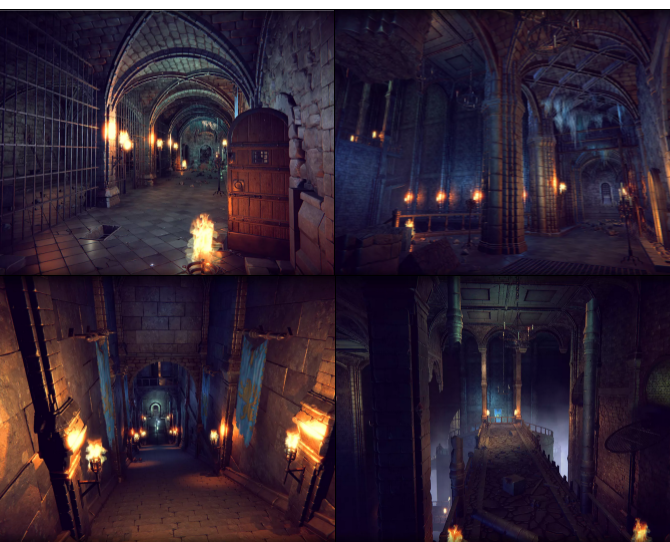
\includegraphics[width=24em]{figures/fig-environment-assets.png}
    \end{center}
    \legend{Source: Collation of screenshots performed by the authors from images captured from the original Unity Asset Store website pages for the \emph{Fantasy Dungeon} Unity asset.}
    \label{fig:environment-assets}
\end{figure}

% Then, we need 3D models for the Characters, The Blacksmith: Characters, Skeleton Zombies and Longsword Animset Pro

In sequence, we require 3D models to represent the playable character and any non-playable entities the player would be able to interact with. Regarding the non-playable entities, we attempt to implement enemy agents comparable to the enemies presented in the early levels of Dark Souls. Most of the enemies in these early sections of the original game are \emph{Undead}\sepfootnote{fn:undead} beings named \emph{'The Hollow'}, which are represented by creatures with decomposed skin and a dehydrated body that resemble the popular representation of \emph{Zombies}. In the original game, \emph{The Hollow} can be seen wearing a variety of attire, including ragged clothes, armored pieces such as cuirasses, pauldrons and helmets, bare skin or even without flesh in their bodies in the form of \emph{Skeletons}.

In addition to the requirement of being in harmony with the aesthetics of the original game, we also used as a criteria for the selection of enemy character models the requirement of serving a specific purpose in enemy behavior design and encounter design. Each enemy agent in our game should have a specific set of actions which can complement the actions of other enemies in a combat encounter. Therefore, we define enemy role archetypes based on the enemies seen in the initial levels of Dark Souls: the \emph{Ghoul}, the \emph{Archer}, the \emph{Swordsman} and the \emph{Assassin}.

Therefore, for the representation of enemy characters that satisfy our aesthetic and design requirements, we elected the asset packs \emph{Skeleton Zombies}, \emph{Longsword Animset Pro}, \emph{Modular Skeleton Archer}, \emph{Modular Skeleton Rogue} and \emph{Skeleton Humanoid}, all of which contain 3D models representing stereotypes of Zombies and Skeletons that resemble the enemies seen in the early stages of Dark Souls, while satisfying the roles we defined for the design of enemy agents in our implementation.

Another motivation for the selection of these asset packs was their compatibility with the \textsc{Mecanim}\sepfootnote{fn:mecanim} system, which standardizes \emph{skeletal rig}\sepfootnote{fn:skeletal-rigs} definitions for animations in humanoid characters in the \textsc{Unity} engine. When compatible with this system, character models can be used in combination with most animations that can be found in the \textsc{Unity Asset Store}, which provides the possibility of choosing from a wide collection of animation sets for multiple purposes, including animations for weapons wielded by the enemy characters we designed for our implementation.

% Figure: Assets used for character models
\begin{figure}
    \begin{center}
    \caption{A mosaic portraying the 3D character models in Bright Souls.}
        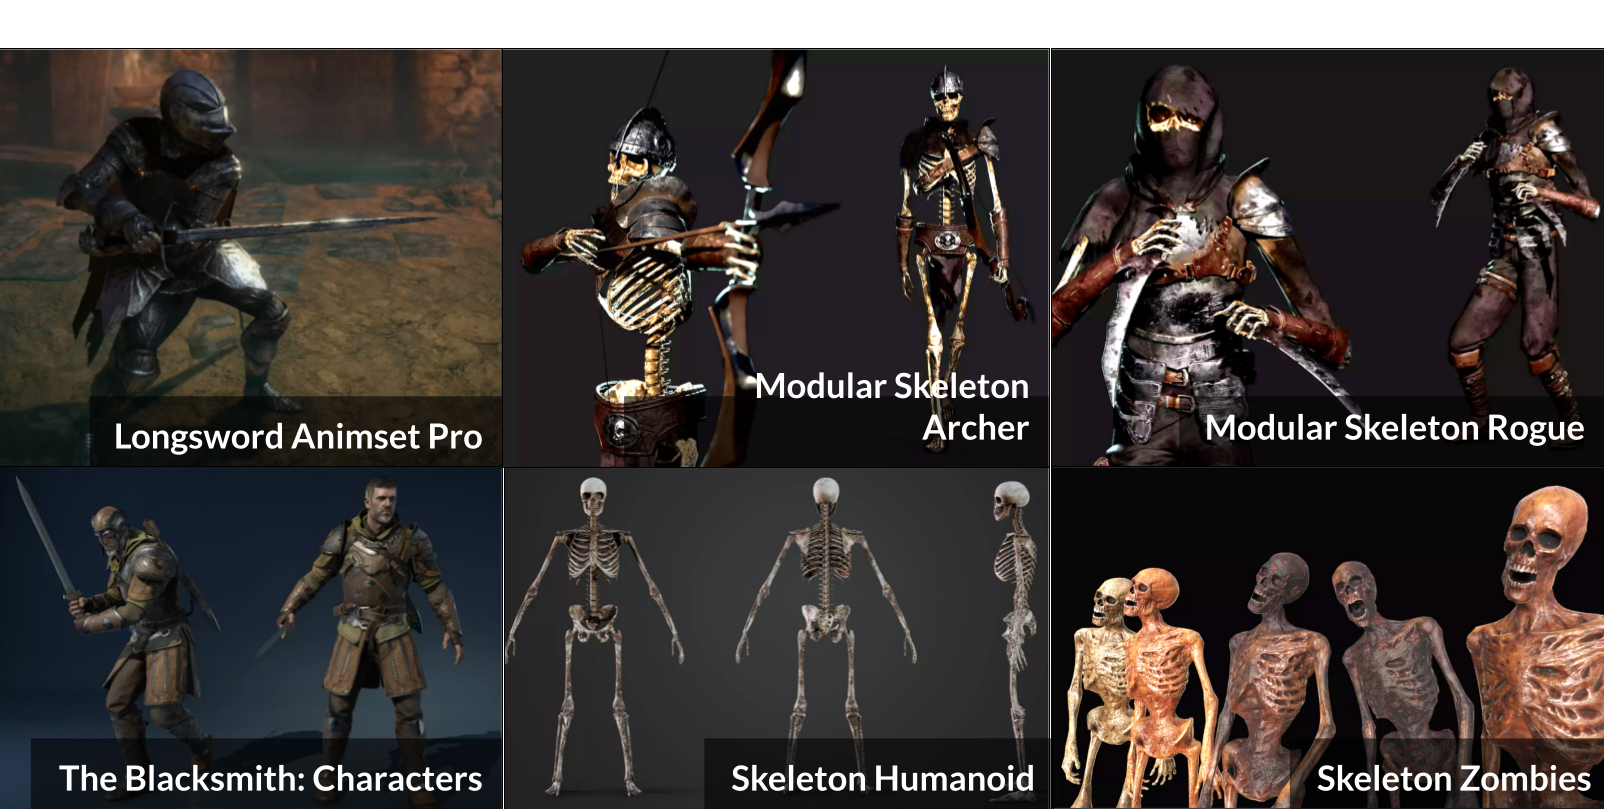
\includegraphics[width=30em]{figures/fig-character-assets.png}
        \legend{Source: Collation of screenshots performed by the authors from images captured from the original Unity Asset Store website pages for each of the assets used in this work.}
    \end{center}
    \label{fig:character-assets}
\end{figure}

% Talk about model for player Character: Blacksmith: Characters
When considering the options to represent the playable character, we must constrain our options to the aesthetic aspects of the Dark Fantasy genre, where a character would need to dress with the appropriate attire or armor pieces and should be able to wield common weapons from a Medieval thematic landscape such as swords and shields. The second criteria considers the gameplay aspects of our implementation, where we constrain the possible features to a definition of a standardized experience from the original game using the most popular equipment setup used by players -- the 'Sword and Shield' combination.

Therefore, we require a 3D model for a humanoid character that can be inserted in the context of a Dark Fantasy world, that can visually satisfy the \emph{Warrior} character archetype wielding a sword and shield, and that is compatible with the skeletal rig for an animation set that contains sword and shield animations. For this purpose, we selected the \emph{Challenger} character model from the \emph{Blacksmith: Characters} asset pack, which portrays a middle-aged warrior wielding a sword and shield and using leather body armor pieces. As with the 3D models selected for non-playable entities, the Challenger character is compatible with the \textsc{Mecanim} skeletal rig system from Unity, which provided compatibility with most animation asset packs from the \textsc{Unity Asset Store}.

% After that, we need animations that can be easily integrated with the designed combat system
To properly integrate the characters into the game world, and to provide visual feedback as to what actions characters are performing given their functional purpose in terms of gameplay aspects, we require animations for humanoid characters that are compatible with the \textsc{Mecanim} system and that are congruent with the purpose of each model. The animation set for each playable or non-playable character should appropriately reflect the weapons and other equipment that the character possesses, as well as the overall body proportions and weight of the attire being used.

An example of animations being congruent with the purpose of a character would be an archer enemy that has animations for wielding a bow, drawing arrows from a quiver and shooting arrows. Since the armor pieces for an archer enemy should be lighter in comparison to a heavy-armored warrior archetype enemy, the movement animations should include faster steps and less restricted joint rotations to reflect the weight of the light attire.

Considering these requirements, we selected the asset packs \emph{ZOMBIE Starter Animation Set}, \emph{Sword and Shield Animset Pro}, \emph{Longsword Animset Pro}, \emph{Archer Animset Pro} and \emph{Rogue Animset Pro}. Each of the animation sets selected for our implementation satisfies the functional requirements of roles designed for playable and non-playable characters, while also being compatible with the skeletal rig standard defined by the \textsc{Mecanim} system.

% Then, we need sound effects and ambient background music that mirror the affective purpose of sound in Dark Souls
We also require sound effects to provide a clear feedback of actions and consequences in the game world, such as a character moving, attacking, blocking an attack, getting hit by an attack or dying. The sound effects for our implementation were selected mainly because of their similarity to the sound effects of the equivalent effects in the original game. For instance, a sound effect for when a character is hit in the original game conveys both the weapon that is being used by the attacker and the scale of damage that is being applied to the target. A frontal attack presents less of a deep, impactful sound effect than a back-stab attack, which does a significantly higher amount of damage. For these reasons, we chose the asset packs \emph{Axe Swing \& Damage Sounds}, \emph{Medieval Fantasy 2 Audio} and \emph{Universal Sound FX} which contain a wide variety of sound effects representing medieval melee weapons such as swords, axes, shields and bows, while also providing a variety of impact levels for successful attacks.

For this project, the immersion of players in the environment of an abandoned castle was also considered, and thus we chose to add ambient background noises and music that could be looped for the duration of a session. As a base requirement for the selection of these noises, it was decided that they should provide a sense of depth to the scenery, with quieter sound effects for events that are closer to the player such as crumbling stone and crackling wood, and somewhat louder sound effects for events that are far away from the player, such as running water, fire and falling chunks of stone. As for the music, it should provide an overall sense of horror and mystery that goes in accordance with the Dark Fantasy genre. Therefore, we selected the asset packs \emph{Medieval Fantasy 2 Audio} and \emph{Dark Fantasy Audio} for ambient sound effects and music, which can appropriately convey the sense of an abandoned, crumbling castle while also containing music for an eerie environment.

% We also need Visual Effects that can go along with the sound effects to provide a proper visual feedback when the player hits an enemy. % 

In sequence, we require a collection of \emph{particle-based}\sepfootnote{fn:particle-vfx} visual effects to provide a proper visual feedback when characters are able to successfully attack their enemies, as well as visual effects that complement the aesthetics and purpose of the 3D models we selected for our environment. For conveying successful attacks, we chose to add pseudo-volumetric particles for a splatter of blood that originates from the body of the attacked target, with the asset pack \emph{Pseudo-Volume Blood Effects} being the most appropriate for this purpose. To increase the detail and depth of our 3D environment, we used fire particle effects for candle and small torches from \emph{Smoke \& Ember FX} and \emph{Unity Particle Pack}. In additional to fire particles, these asset packs also provided smoke particle effects, which were used to both complement the fire from light sources and to help occlude certain parts of our levels until the player moved to a closer position.

% We need 2D UI Elements that can convey the basic gameplay resources: Health and Stamina
We also need a collection of 2D UI Elements that are able to convey the basic gameplay resources that the player should be able to keep track of during a gameplay session: \emph{Health} and \emph{Stamina}. For this purpose, \emph{Health Bars} will suffice as they are a common standard for representing attributes that have a variable maximum value and a minimum value of zero. The design and layout of these elements should be in overall accordance with the Dark Fantasy genre, avoiding overly saturated color pallettes and an exaggerated geometric complexity.

% We also need UI Elements for menus, settings, tooltips and button captions
We also require a variety of UI elements that can be used for assembling the menus that will be used by the player to initiate sessions, pages for the configuration of game settings, small tooltips that provide a brief description of the functionality of UI elements, and button captions that can be displayed during a game session to provide the player with a reference of the actions that can be performed at any given time.

To represent most of the UI elements in our implementation, we selected the asset pack \emph{RPG \& MMO UI 5} which contains the most common UI elements used in the video games such as menus, buttons, tooltips, Health bars, loading screens and portraits, with an overall design tailored for Fantasy games. This asset pack also contains an under-saturated color palette with greyed out colors, which goes in accordance with our aesthetic needs for a Dark Fantasy game. For button captions, we selected the asset pack \emph{PC \& Consoles Buttons Icons} which contains button icons for a multitude of input devices such as Xbox Controllers, PlayStation Controllers, Mouse \& Keyboard and even joysticks for Head-Mounted devices.

% Finally, we used complementary editor tools that allowed for a more concise and streamlined workflow for serializing game data and implementing common functionality for third-person hack and slash games
We also included \emph{Odin Inspector} as a complementary editor tool that allowed for a more concise workflow when serializing game data such as character attributes, physics properties and gameplay values into binary game asset files. With \emph{Odin Inspector}, it was possible to create reusable serializable classes that could be assigned to components directly from the \textsc{Unity} engine editor, which was used as a base for the creation of our \emph{Attributes}, \emph{State Machines} and \emph{Performance Tracking} systems.

% Table showing Asset Name, Type, Size, Price, Path in Project
In conclusion, we use table \ref{tab:table-game-assets} to provide a consolidated list of the assets discussed in this section, along with the appropriate extraction paths for the assets to work with our source code.

% Table: List of game assets
\begin{table}[!h]
    \begin{center}
      \caption{A consolidated list of the assets used in the implementation of this work.}
      \label{tab:table-game-assets}
      \rowcolors{2}{}{gray!25} % Alternate row colors
      \begin{tabular}{ >{\small}w{l}{11em} >{\small}w{c}{4em} >{\small}w{c}{3em} m{13em} } % alignments and column size
        \addlinespace
        \toprule
        % Headings
        \textbf{Name}                & \bf Type  & \bf MSRP & \textbf{\small Path in Project}                             \\
        \midrule
        % 3D Models
        Fantasy Dungeon              & 3D Models &  \$90.00 & \texttt{\tiny Assets/AssetStore/3D/FantasyDungeon/}      \\ 
        Skeleton Zombies             & 3D Models &  \$16.00 & \texttt{\tiny Assets/AssetStore/3D/StudioNewPunch/}      \\
        Modular Skeleton Archer      & 3D Models &  \$34.99 & \texttt{\tiny Assets/AssetStore/3D/SkeletonArcher/}      \\
        Modular Skeleton Rogue       & 3D Models &  \$34.99 & \texttt{\tiny Assets/AssetStore/3D/SkeletonRogue/}       \\
        Skeleton Humanoid            & 3D Models &  \$19.99 & \texttt{\tiny Assets/AssetStore/3D/SkeletonHumanoid/}    \\
        The Blacksmith: Characters   & 3D Models &     FREE & \texttt{\tiny Assets/AssetStore/3D/ChallengerCharacter/} \\
        \midrule
        % Animations
        ZOMBIE Starter Animation     & Animation &   \$4.99 & \texttt{\tiny Assets/AssetStore/3D/ZombieAnimset/}       \\
        Sword and Shield Animset Pro & Animation &  \$65.00 & \texttt{\tiny Assets/AssetStore/3D/SwordShieldAnimset/}  \\
        Longsword Animset Pro        & Animation &  \$50.00 & \texttt{\tiny Assets/AssetStore/3D/LongswordAnimset/}    \\
        Archer Animset Pro           & Animation &  \$55.00 & \texttt{\tiny Assets/AssetStore/3D/ArcherAnimset/}       \\
        Rogue Animset Pro            & Animation &  \$50.00 & \texttt{\tiny Assets/AssetStore/3D/RogueAnimset/}        \\
        \midrule
        % Sound effects and Music
        Axe Swing \& Damage Sounds   & SFX       &   \$5.00 & \texttt{\tiny Assets/AssetStore/Audio/AxeSwingSounds/}   \\
        Medieval Fantasy 2 Audio     & SFX       &  \$50.00 & \texttt{\tiny Assets/AssetStore/Audio/MedievalFantasy2/} \\ 
        Universal Sound FX           & SFX       &  \$40.00 & \texttt{\tiny Assets/AssetStore/Audio/UniversalSoundFX/} \\
        \midrule
        % Music
        Dark Fantasy Audio           & Music     &  \$22.99 & \texttt{\tiny Assets/AssetStore/Audio/DarkFantasyAudio/} \\
        \midrule
        % Visual Effects
        Pseudo-Volume Blood Effects  & VFX       &  \$15.00 & \texttt{\tiny Assets/AssetStore/VFX/KriptoFX/BloodFX/}   \\ 
        Smoke \& Ember FX            & VFX       &  \$10.00 & \texttt{\tiny Assets/AssetStore/VFX/SmokeEmberFX/}       \\ 
        Unity Particle Pack          & VFX       &     FREE & \texttt{\tiny Assets/AssetStore/VFX/UnityParticlePack/}  \\
        \midrule
        % UI Elements
        PC \& Consoles Buttons Icons & UI        &  \$14.99 & \texttt{\tiny Assets/AssetStore/UI/PCConsolesIcons/}     \\ 
        RPG \& MMO UI 5              & UI        &  \$35.00 & \texttt{\tiny Assets/AssetStore/UI/RPGMMOUI5/}           \\
        \midrule
        % Editor Utilities and Extensions
        Odin Inspector               & Plugin    &  \$55.00 & \texttt{\tiny Assets/Plugins/Sirenix/}                   \\ 
        \bottomrule
      \end{tabular}
    \end{center}
  \end{table}

% ============================================================================
% ============================================================================
% ============================================================================

\subsection{Gameplay Mechanics and Systems}

% Overview of all gameplay subsystems
% - Here we talk about the subsystems that involve the player-controlled character in our implementation and how it interacts with non-playable entities
% - Figure: Player components and class diagram
% - Movement mechanics with collision handling for walls and obstacles, detection of slope thresholds and handling of gravity and fall damage
% - A character animation systems that reacts to actions performed by the player and any events that might affect the status of the player, such as hits taken, staggering and death
% - A third person camera that allows the player to orbit the viewport around the game character, while also constraining its position and viewport contents to the boundaries of a playable environment
% - A lock-on camera that is able to frame the player and a target enemy character, and which is coupled with a target prioritization system for enemy characters, and that allows the player to switch targets
% - A combat system which handles hit and block detection, combat effects such as stamina draining, damage and poise break, attack action and state handling, and combat statuses that affect the ability of a character performing actions
% - An attributes system that can be containerized into components for game entities, is able to serialize value data types, broadcasts events when its values are changed, and can be used by other gameplay subsystems to determine the status of a game entity
% - A character status system that accounts for Invincibility Frames (IFrames) when dodging and the inability of performing actions when staggered or dead

% ============================================================================
% ============================================================================
% ============================================================================

% Movement mechanics and physics
\subsubsection{Movement mechanics and physics}

% - CharacterController for wall and obstacle collision and running over slopes

Traditionally, the movement for player-controlled characters in games is not made to be physically realistic. Characters will often move at abnormally high speeds, are able to stop almost immediately and can turn their movement direction with ease. This is made so that character movement is highly responsive to player input and becomes easier to manipulate in comparison to physics-based controls. If player characters in video games were to be physically accurate, they would take significant time to accelerate to their maximum movement speed and decelerate until stopped, while also having difficulty turning sharp angles at high speeds.

For gameplay purposes, characters implemented with physical accuracy feel heavy and difficult to control, forcing the player to consider  physical properties of their characters and the geometry of the environment. This causes a significant amount of overhead for the player to obtain proficiency with motion controls. In general, character movement should be a streamlined, trivial mechanic that can be quickly learned by the player. Learning motion controls in a game should not get in the way of the player partaking into the core gameplay loop\sepfootnote{fn:core-gameplay-loop}, unless movement in itself is part of the core game loop as in \emph{Death Stranding}\sepfootnote{fn:death-stranding}.

Considering the need for responsive movement that can be easily mastered, we use the implementation of a \emph{CharacterController}\sepfootnote{fn:character-controller} component that is natively built-in as part of \textsc{Unity}'s base functionality. CharacterControllers are not affected by Unity's physics system, are able to slide along walls when moving against them over a non-orthogonal angle, to detect and move over small vertical offsets in ground geometry such as steps and ledges, and to handle movement in slopes.

The movement input from a player will generate different motion types depending on camera state. In the default state of a Third-Person Orbital Camera, movement input will cause the player character's body to rotate to face a direction relative to the camera's viewport, while also causing the body to move forward according to its current rotation. The Movement System broadcasts the signal that the player is always moving forward, which is received and handled by the Animation System. In this camera state, motion itself is handled by the animations so that the movement speed perfectly matches the animation being played and avoiding \emph{movement drifting}\sepfootnote{fn:movement-drifting} issues.

While this setup of the Movement System handling body rotation and the Animation System handling motion itself does cause the player to move in the direction defined by their input, this also requires a \emph{maximum rotation speed} to be taken into consideration. A character should be unable to immediately turn to the opposing movement direction, with the \emph{maximum rotation speed} constraining the speed at which a player is able to turn.

In the state where the player performs a \emph{Lock-On}\sepfootnote{fn:lock-on} targeting an enemy character, movement input causes the player to directly move at a direction without changing its body rotation. In this state, body rotation is handled by the camera system, where the player-controlled character will always face an assigned target. The Animation System will use movement input to blend between multiple movement animations such as forward movement, side steps and back steps. Movement motion in this state is still relative to viewport direction, but the viewport in itself is positioned relative to the player and their target. Camera positioning for \emph{Locked-On Cameras} will be further explained in subsection \ref{sec:lock-on-camera}.

Another state that should be considered for motion controls is when the player is not touching the ground. In technical terms, the Capsule-shaped \emph{collider}\sepfootnote{fn:colliders} from the player CharacterController would not \emph{overlap}\sepfootnote{fn:collider-overlapping} with ground geometry. In this situation the player character should be considered "On-Air", and movement input should have less of an influence in motion and body rotation or no influence at all, as being able to accelerate, decelerate and quickly turn without ground friction would be considered implausible by players and could possibly break immersion. When the player is not on ground, we constantly accelerate our CharacterController velocity by a gravity vector on fixed time steps defined by the \emph{FixedUpdate}\sepfootnote{fn:fixed-update} event of the \emph{MonoBehaviour}\sepfootnote{fn:monobehaviour}.

% - Gravity and grounded state detection

To detect if a player is ground or not, we make use of \emph{Unity's} built-in \emph{SphereCast} operation, which iterates performing multiple overlaps of a sphere with a radius slightly higher than the radius of our CharacterController with the ground geometry, along a direction defined by a \emph{Ray}\sepfootnote{fn:rays}. The ray originates from the center of the body of the player-controlled character, and extends along the direction of the gravity vector in a length of three quarters of the vertical size of the CharacterController capsule collider. This is done so that vertical collisions can be detected ahead of time when the player is falling at high speeds, avoiding the common problem in video game physics where the player becomes stuck inside ground geometry.

\begin{lstlisting}[caption={Implementation of grounded state detection.},label={lst:grounded-detection}]
var ray = new Ray(transform.position, Vector3.down);
grounded = Physics.SphereCast(ray, charController.radius + 0.1f, charController.height / 2f + 0.5f, physicsData.GroundDetectionLayers.value);
// Animator also applies gravity, so when not grounded disable animator physics
player.Anim.applyRootMotion = grounded;
\end{lstlisting}

An advantage of using \emph{Raycast-type}\sepfootnote{fn:raycasts} operations instead of frame-by-frame collision overlap detections is that Raycasts are able to precisely detect the points where a collider starts overlapping with the ray along a fixed length of an axis. This enables us to pinpoint which parts of our collider the ground geometry touches and the exact moment the ground geometry first makes contact with our character, being the optimal operation to use when considering objects that are moving along an axis over time -- which is the case for the player being affected by gravity in our implementation.

In contrast to using a regular Raycast, the SphereCast operation is able to detect overlaps in a volume, which means that complex collider setups which overlap in the borders of our CharacterController will still be detected. A common situation in games where platforms and gravity can affect the player is that players might find themselves over one or multiple ledges, where a single Raycast operation would not be able to handle colliders that are in the edges of a CharacterController.

% Figure: Example showing visual difference of Raycast vs SphereCast

In games where grounded-state detection is not handled appropriately, Character controller components will often accumulate vertical velocity indefinitely, since while being impossible to move downwards due to the character controller constraining movement against colliders, the 'grounded' state is never detected. What commonly happens after this is that when the player steps away from the ledge sufficiently, they will instantly fall to the ground instantly because of the accumulated speed. If the game is programmed to apply fall damage in this situation, this might mean instant death even though the player did not fall from a considerable height.

Finally, in the frame where a character that was previously considered not groun\hyp{}ded detects ground collision, we invoke the \textsc{OnHitGround} event, and proceed to perform fall damage calculation. In our implementation, fall damage is calculated by considering fall speed multiplied by a parametrized speed-to-health-point conversion factor, named 'FallDamageMultiplier'.

Figure \ref{fig:movement-class-diagram} shows an overview of the class architecture for our implementation of the movement system. We have a top-level \textsc{Player} class which holds the components for all gameplay-related subsystems. The \textsc{PlayerMotor} component is an implementation of the \textsc{ICharacterMotor} abstraction, and is responsible for implementing the movement and physics logic of our motion controls.

When input is received from the user, the \textsc{PlayerMotor} component filters the input, calculates movement direction based on viewport orientation, and redirects the actual transform position changing to \textsc{Player.Move()}. The \textsc{Player} class in turn calls \textsc{CharacterController.Move()} that considers collisions and other physics-related constraints, and broadcasts movement signals that will be consumed by the \textsc{PlayerBody} class, which is responsible for handling character animation.

% Figure: Player Movement Class Diagram for Bright Souls
\begin{figure}[!ht]
    \begin{center}
    \caption{Class diagram representing the architecture of our Movement System.}
    \vspace{0.5em}
        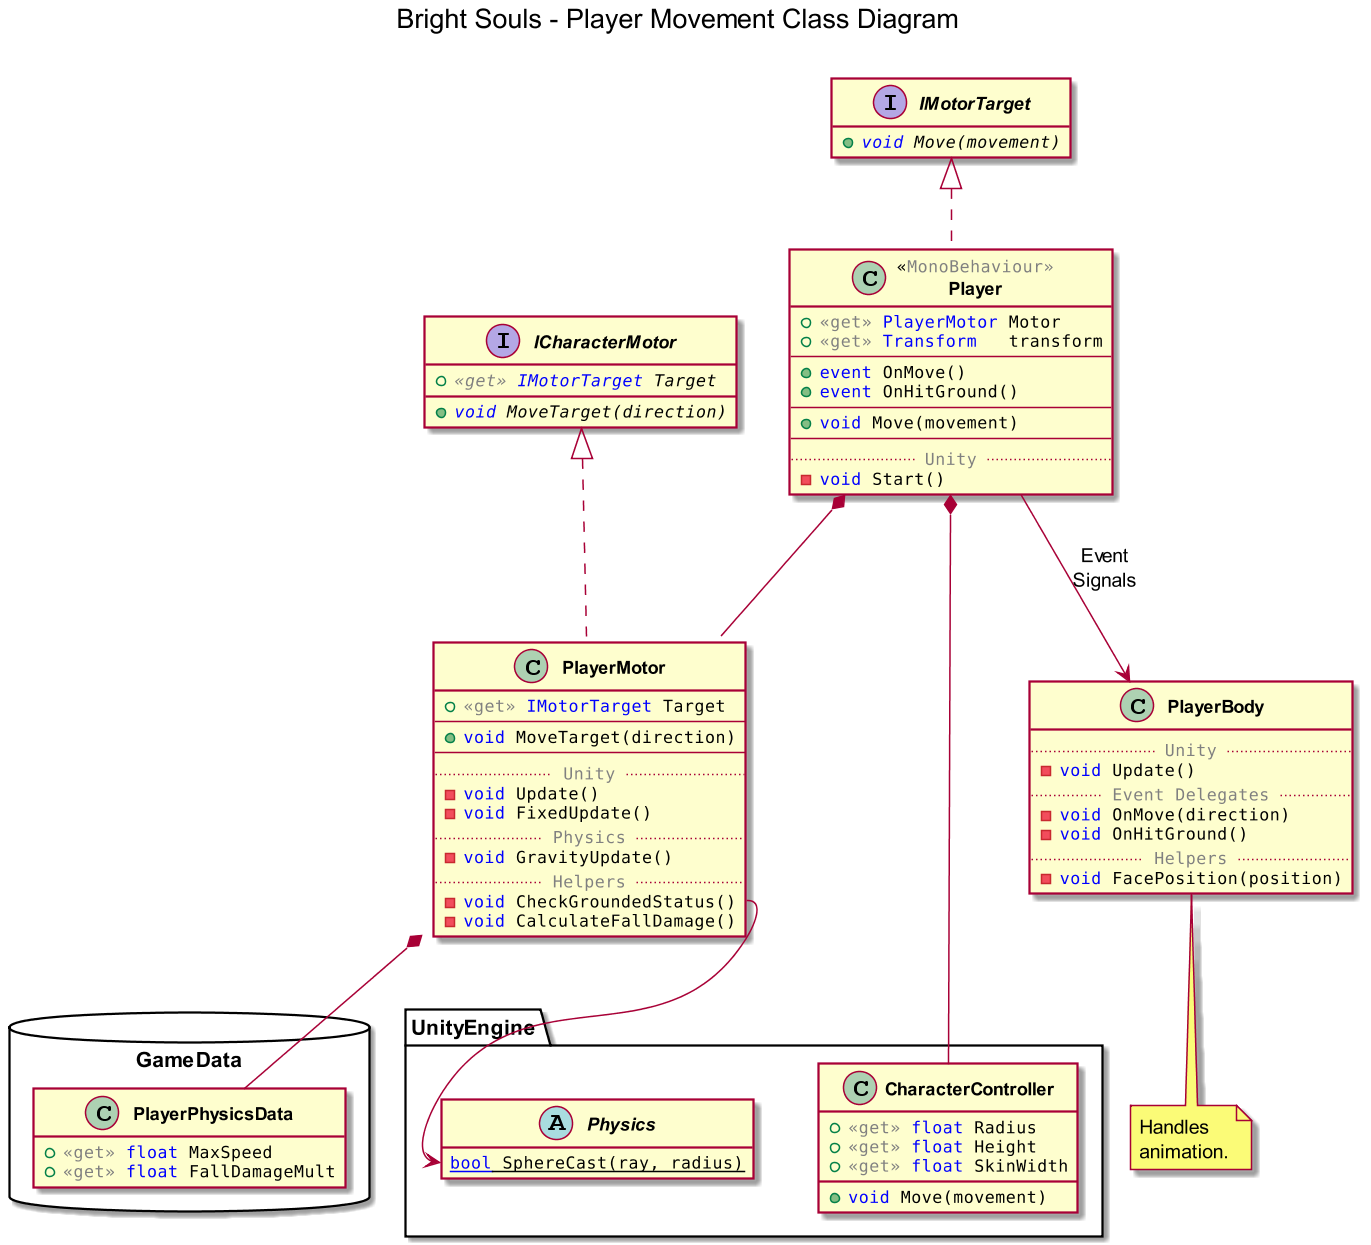
\includegraphics[width=34em]{figures/fig-player-movement-class-diagram.png}
        \legend{Source: Diagram assembled by authors.}
        \label{fig:movement-class-diagram}
    \end{center}
\end{figure}

% ============================================================================
% ============================================================================
% ============================================================================

\subsubsection{Camera System}
\label{sec:lock-on-camera}

% In this implementation, we design and implement two separate camera modes
%   - Orbital Third Person Camera
%       > Commonly used for third person hack n' slash or platforming games
In our implementation, we use our analysis of \emph{Dark Souls} in section \ref{sec:analysis-dark-souls} to design two separate camera modes with complementary functionality that can be used as tools for the player to achieve optimal performance in and out of combat. First we implement an \emph{Orbital Third Person Camera}, which is commonly used in third person \emph{Hack and Slash} and \emph{Platforming} games where the player has to evaluate the properties of the environment they are in and quickly assess dangers that might cause their defeat to devise a plan of action.

%       > Camera positions itself in the perimeter of an ellipsoid that is centered on the player
%       > Input from the player generates movement along the perimeter, causing the camera to orbit around the player
%       > Attempts to frame both the player and the environment by using a position above the player as pivot
An Orbital Third Person Camera positions itself in the perimeter of a three dimensional ellipsoid that is centered on the player, where input from the player generates movement along this perimeter. This type of camera attempts to frame both the player and the environment at the same time, having the player on a central position in the screen and using a position above the player as a rotation pivot. The rotations from player input along with the framing algorithm causes the camera to perform an orbital movement.

%       > In our game, it is the default camera mode, used for traversal around the map
%       > Free control over framing enables player to scout for enemies, avoid pitfalls
In our game, Orbital Third Person Cameras are the default camera mode, and are mainly designed for traversal around the three-dimensional environment. The fact that the player has control over the positioning and framing of the camera enables the player with the possibility to scout the environment for pitfalls and enemies before performing movement. This is the perfect type of camera to be used in out-of-combat situations in third person games, as players can gather information safely and use it to devise a plan-of-action.

%   - Lock-On camera
%       > Mostly used in action third person hack n' slash games that have melee combat, although some RPGs also use it
%       > Camera positions itself behind the player and attempts to frame both the player and a target character
The second type of camera in our implementation is the \emph{Lock-On Camera}, which is mostly used in action third-person \emph{Hack and Slash} games that have melee combat. This type of camera positions itself behind the player character, and attempts to frame both the player and a target -- most commonly an enemy character. Whenever the target character moves, the camera adjusts its position and framing to maintain a fixed relative positioning between the player character and their target.

%       > Camera positioning and framing creates fixed "dimensions of movement" of the player relative to a target,
%         making it easier for a player to avoid attacks from that target and find the optimal spacing to land their
%         own attacks
The relative positioning and framing of a Lock-On Camera creates fixed axes of movement between the player character and their target where if a player moves horizontally, they will move in a circle around the target character. Moving forward and backwards adjusts the distance between the player and their target. The purpose of this mechanism is for the player to have better control of spacing during combat, making it easier for the player to avoid attacks and find the optimal distance to land their own attacks.

%       > Useful for the player to be able to track and attack a single target with ease without missing,
%         instead of having to specify a "direction" for the attack, the player can simply press the attack button
%         and the character will already be facing the enemy and perform the attack in the correct direction
The fact that a Lock-On Camera is always facing a single target character removes the necessity for players to specify a direction for their attacks through input. Instead, players can simply press the attack button when their characters are within attack range. Since the character is constantly facing the enemy, the direction of their attack is guaranteed to be correct. Another positive effect caused by this behavior is that the framing helps the player to focus on the actions being performed by the enemy character, helping to understand when an enemy is attacking and which kind of attack an enemy is performing.

%       > Has issues in environments in constrained spaces, where the enemy is too close to the player or the player
%         is too close to a wall. Framing becomes an issue in this case
However, Lock-On camera implementations face issues when the target character is too close to the player character, or when they are operating in environments with constrained space. When the player character is too close to their target, it is common for Lock-On cameras to not adjust their vertical offset, meaning that the framing direction must be angled downwards and into the ground. This causes the player to have limited geometric information about the surroundings of both characters, making it harder to efficiently navigate the environment during combat. Furthermore, if a player is moving horizontally when close to their target, the perimeter of the circle of movement has a significantly reduced radius, making the camera rotate at high speeds and causing motion sickness\sepfootnote{fn:motion-sickness} in some instances.

When Lock-On cameras operate in constrained space, it is common for the default offset position to be located outside the playable space (e.g. inside walls), and thus a position resolution algorithm is required to guarantee that the camera is always in a valid position. The most common algorithm is the pull-forward approach, where if the camera would be located outside the playable space the target position is recalculated so that the camera is brought closer to the player. While this solution works until a certain point, if the player positions their character too close to a wall it might create a situation where it is impossible for the camera to frame both the player and their target, with either the player character occluding the target or the camera focusing solely on the target by being positioned above the player character. In addition, a similar problem to that of players being to close to targets occurs, where in this case the camera might reposition too quickly due to the resolution algorithm.

Figure \ref{fig:camera-types} shows a comparative diagram of both camera types implemented in this work, where four screen captures are used for the Orbital Third Person Camera to illustrate multiple framing angles that can be achieved from player controlled rotations.

% * Figure: Orbital and Lock-On camera framing/rotation
\begin{figure}[!ht]
    \caption{Comparative screenshots showing the difference between the Orbital and Lock-On camera modes.}
    \vspace{0.5em}
    \begin{center}
        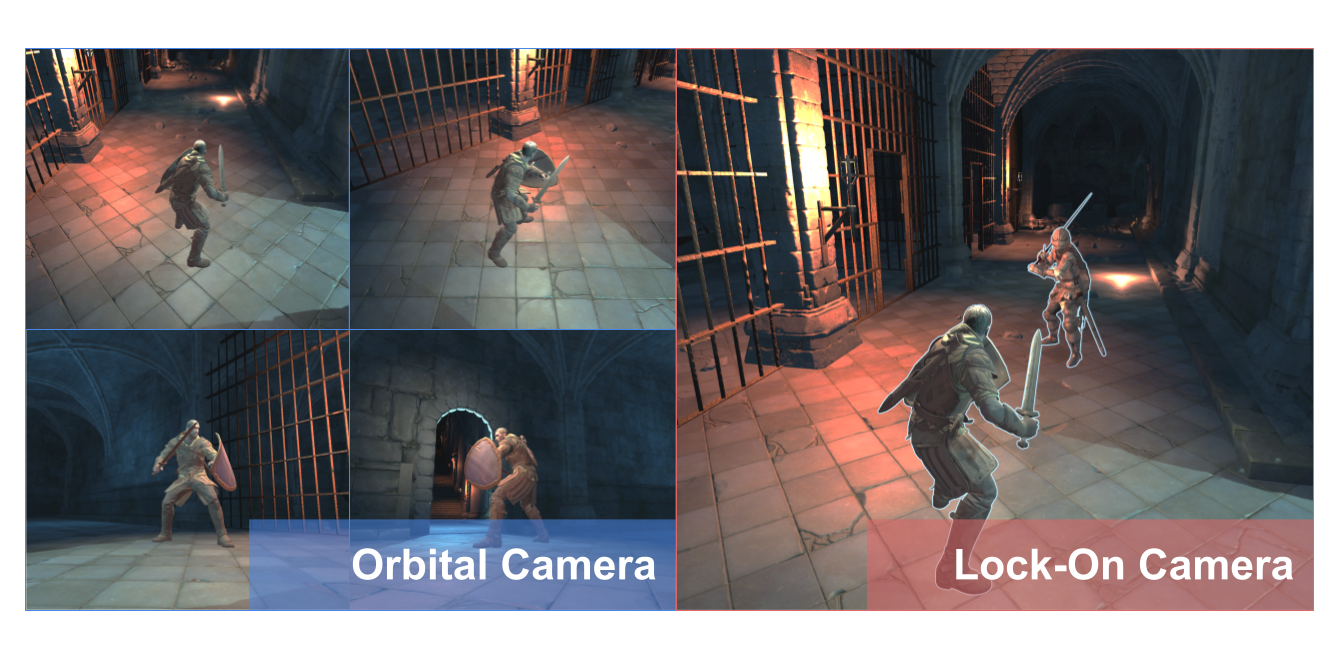
\includegraphics[width=34em]{figures/fig-camera-types.png}
    \end{center}
    \legend{Source: Screen capture of application developed by authors.}
    \label{fig:camera-types}
\end{figure}

% Third Person Orbital Camera implementation
% - Use of Cinemachine
%     - Ready-to use implementation of orbital rotation with parametric spline curve for vertical axis
%     - Smooth transition between virtual cameras which was useful for Orbital Camera and Lock-on modes
Regarding the implementation of the Orbital Camera, we chose to use the \emph{Cinemachine} Unity Package due to its comprehensive API and functionality for multiple types of cameras, including specific algorithms to manipulate Orbital Cameras. Another useful trait is that the APIs provided by Cinemachine enable defining parametric curves for positioning, which increases the expressive power of game designers.

%     - Algorithmic motion that can simulate cinematic behavior with camera shake effect and framing corrections
Cinemachine can also manage, compose and blend multiple cameras, which is useful to perform shot transitions triggered by a signal system that resembles the \emph{Observer} pattern\sepfootnote{fn:observer-pattern}. Cinemachine also includes algorithms for procedural motion generation, which is used to create screen shake effects with high fidelity when the player is attacked by an enemy, or to properly adjust framing when the camera needs to track movement of high velocity targets.

% Prefab GameObject hierarchy with CinemachineBrain at root 
% MainCamera object as a child of the CinemachineBrain
We start by creating a \textsc{Prefab}\sepfootnote{fn:unity-prefabs} hierarchy of \textsc{GameObjects}\sepfootnote{fn:unity-gameobjects} where we include a \textsc{CinemachineBrain} component in the root level, and multiple \textsc{VirtualCameras} as child objects. The \textsc{CinemachineBrain} component is responsible for defining the current active camera, camera transitions and the signals that trigger each transition. The \textsc{CinemachineBrain} brain component requires a reference to a \emph{Main Camera}, a special \textsc{GameObject} with a \textsc{Camera} component responsible for rendering the final output of our camera management system. We add the \emph{MainCamera} object as a child of the root.

% VirtualCamera child objects that contain definitions for transposing and composing strategies
As child GameObjects of the hierarchy root, we include a set of \textsc{VirtualCameras} for each of the camera modes in our implementation. In this case, we simply add a VirtualCamera for the Orbital Camera and another for the Lock-On Camera. VirtualCameras are Cinemachine abstractions that define the physical properties of a camera along with transposing and composing strategies\sepfootnote{fn:transposing-and-composing}. In this case, we use a VirtualCamera with an Orbital transposing strategy and a single LookAt target aiming at a pivot position above the player character. For the Lock-On camera, we use a simple Follow strategy for transposing and a Group Composition strategy to frame both the player character and their target enemy.

% PlayerCameraDirector component, which is responsible for receiving signals from player and translating them into signals for the CinemachineBrain and activating and deactivating PlayerCameraBehaviours
We also add a \textsc{GameObject} containing a \textsc{PlayerCameraDirector} component, which is responsible for receiving signals from the \emph{Player} component and translating them into signals for the \textsc{CinemachineBrain}. The signals are then used to switch and transition between shots. The \textsc{PlayerCameraDirector} is also responsible for enabling and disabling \textsc{PlayerCameraBehaviour} components, which receive player input, manage camera framing targets and initialize camera states.

The \textsc{VirtualCamera} components are tasked with receiving player input and performing the appropriate actions given the input. For instance, the \textsc{OrbitalCamera} receives a two-dimensional vector as input, which is translated into vertical rotation and translation for the Y axis and horizontal for the X axis. In the Lock-On camera, the horizontal axis of the vector input is used to switch Lock-On targets. Figure \ref{fig:camera-class-diagram} shows an overview of the class relationship in our camera system implementation, as well as the signals that are being sent and listened to.

% * Figure:  Camera system class diagram
\begin{figure}[!ht]
    \begin{center}
    \caption{A diagram showing the class relationship of our Camera System implementation, along with the signals being sent and processed.}
    \vspace{0.5em}
        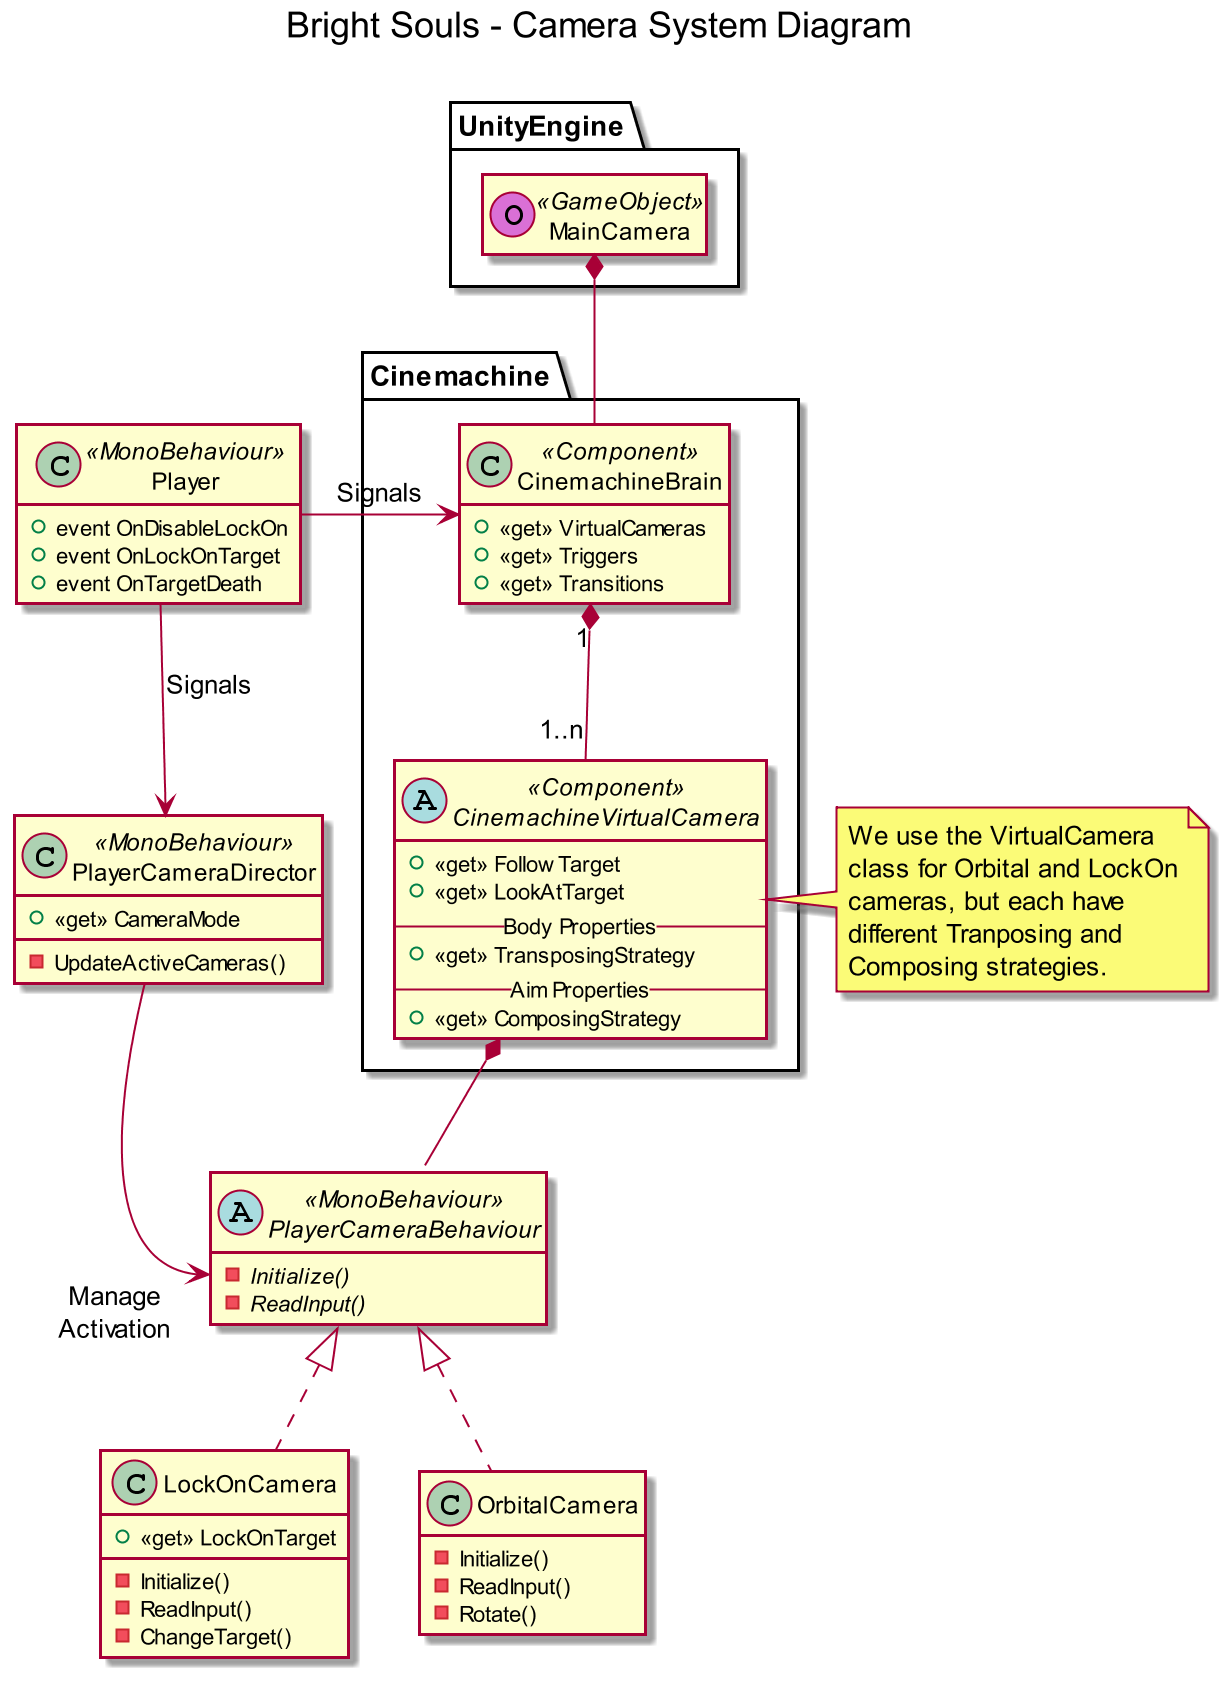
\includegraphics[width=34em]{figures/fig-camera-system-class-diagram.png}
        \legend{Source: Diagram assembled by the authors.}
        \label{fig:camera-class-diagram}
    \end{center}
\end{figure}

%     - Simplified collision geometry enables using a pull-forward collision resolution
For position resolution, we created a simplified and invisible collision map to define the constraints of where a camera can be positioned in a game level. This is done to both improve the performance of raycasts and to avoid jittery movement when using pull-forward collision resolution on thin objects. This collision map is limited to interact with camera algorithms, and does not affect player movement or any other physics entities in any way.

% Lock-On camera and targeting system
% - Possible Lock-on targets must be located in an intersection of the camera viewport with a collision sphere centered at player character
% - Lock-On target prioritization is higher for targets that are closer to the player and to the center of the screen
To detect Lock-On eligible targets, we use a spheric collider in a radius around the player collider and intersect any detected entities with those present in the viewport, to constrain selection to entities being visualized. Eligible targets are collected into a list ordered by distance to the player character, which is updated every second. This is done because targets that are closer to the player are considered a higher threat, as they are more likely to hit the player when attacking.

% - Use of horizontal input axis from Orbital Camera to switch between targets
Horizontal input from the player is used to switch between targets, where moving the input axis to the left switch to the closest target at the left of the current Locked-On target, using coordinates relative to viewport space. Therefore, the position of the next target is selected using a comparison of the position of the entity in the X-axis when converting their coordinates to a viewport space.

% ============================================================================
% ============================================================================
% ============================================================================

\subsubsection{Attributes System}

% Attributes system
Attributes are our abstraction for runtime data that represents the current state of a gameplay entity, such as the Player Character, an Enemy Character or even an interactable object in a level such as a door. Attributes can be initialized, serialized and monitored by external components and are used by a multitude of gameplay related systems. In our implementation, attributes are mostly used to represent combat related variables such as Health, Stamina and Poise, and thus are affected by events triggered by the combat system, such as Stamina being used when the player attempts to attack an enemy, or the Health lost when an enemy succesfully hits the player.

% Based on Generics: Attributes can be generated for any primitive type, such as int, float, double, string.
%   - Serialized into binary gameplay data files for game designers to define the default and maximum values for character health, stamina and poise
%   - Initialized by persistent data managers to maintain player status when transitioning between levels
Attributes are based on \textsc{C\#} \emph{Generics}, and can be generated for any value type such as integers, floating point variables, strings and enumerations. This limitation is imposed in our architecture so that attributes can be easily serialized into binary data files that can be used to define the default and maximum values for each attribute holder. This constraint also facilitates Attribute initialization, which is useful to support persistent data such as maintaining attributes between levels  or loading the state of an entity from a file in a savegame system. 

%   - Monitored by UI systems to display relevant data about the status of the player, for instance a Health Bar that display the current health of the player and shows health lost when getting attacked.
All Attribute types implement the \textsc{IAttribute} interface, which exposes acessors for data manipulation and events for value changes. This facilitates the use of attributes by separate, independent systems in our architecture. For instance, Attributes are monitored by UI (User Interface) systems to display relevant data about gameplay entities, such as the status of the player. Health bars show the current player health and also provide a good estimation of health lost when getting attacked by an enemy using a secondary, trailing health bar.

The advantage of creating of an event monitoring system between Attributes external systems is that upon initial conception of the architecture, we do not exactly know how many components will require communication with each gameplay entity. For instance, when implementing the UI for the player character we can initially propose a single health bar that would simply read the value of runtime variables from the \textsc{Player} class, but if we iteratively add new elements such as floating text, combat messages and visual effects, each of these systems should have direct access to the components that hold data regarding player state, which enforces component coupling in our architecture. With an event system, we can simply subscribe to signals being sent by attributes, constraining the exposed data and methods and facilitating component decoupling.

% - AttributesContainers
%     - Containerization of attributes to allow for entities with different attribute configurations without defining static types
%     - Possibility to dynamically assign attributes during the course of a session, which can be useful for a telemetry system
% - Definition of interfaces that expose attributes to any of the classes that might require it
Attribute owners will often contain different sets of attributes to satisfy the requirements of the systems they interact with. As such, characters that can partake into combat encounters will present different attributes in relation to interactable objects such as doors. To provide a standardized interface for the access of attributes over different entity types, we containerize attributes into \emph{Attribute Containers}, which provide a public interface for dynamic access and manipulation of statically typed attributes contained within an entity. Figure \ref{fig:attributes-diagram} shows an overview of the class relationships in the Attributes System, along with examples of how attributes signalize changes to external components such as UI Elements.

% * Figure: Attributes system class diagram
\begin{figure}[!ht]
    \begin{center}
    \caption{Class diagram for the Attributes System, showing examples of signals being used by UI Elements.}
    \vspace{0.5em}
        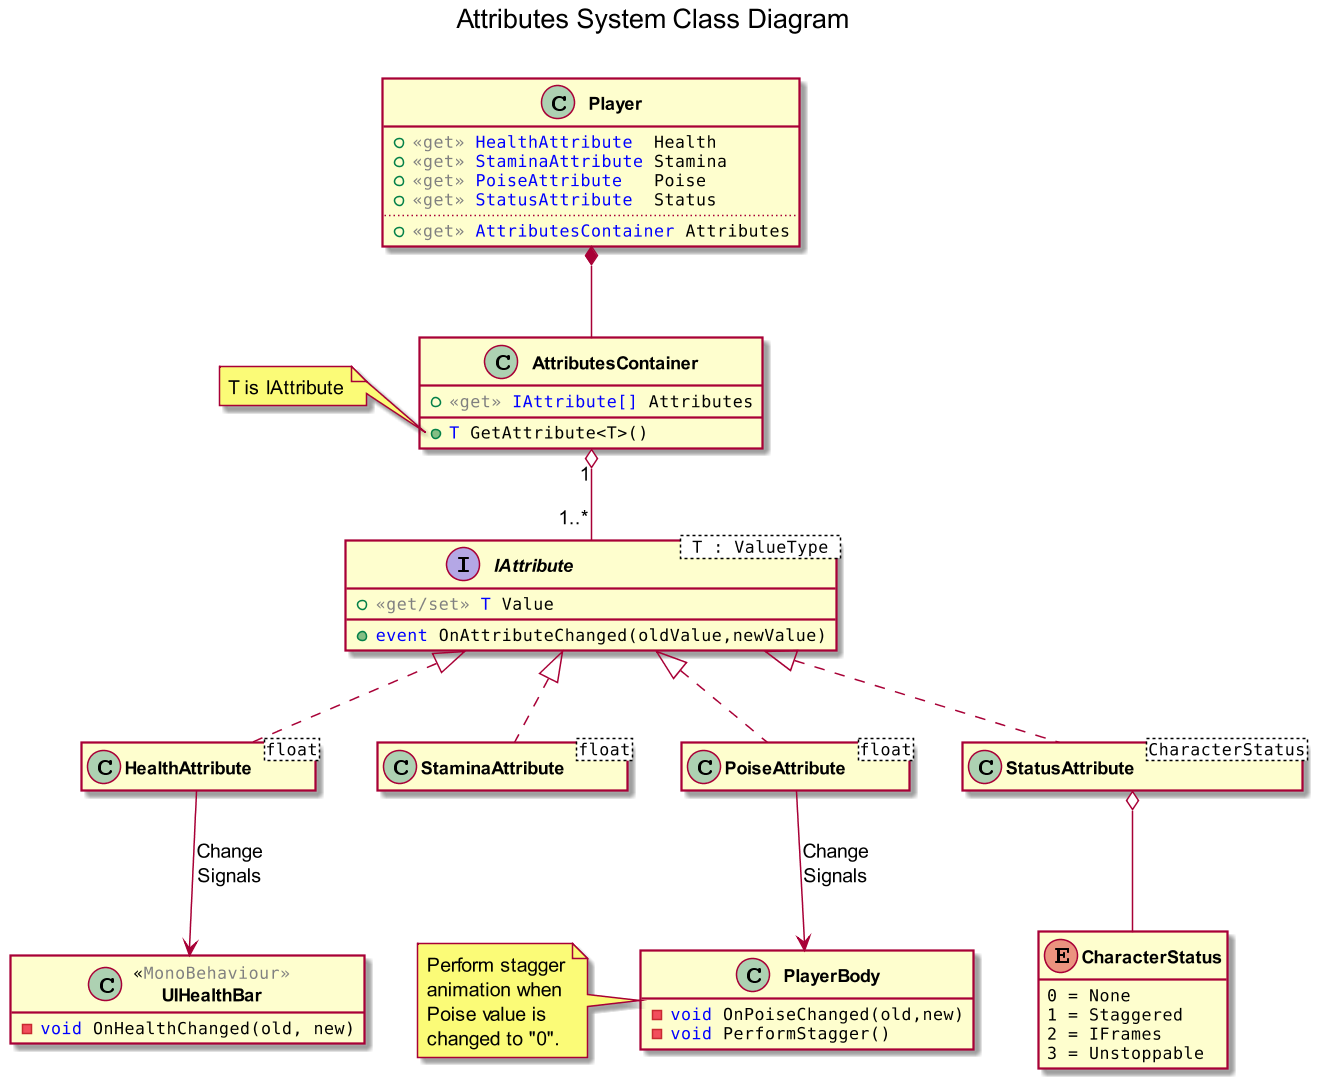
\includegraphics[width=34em]{figures/fig-attributes-diagram.png}
        \legend{Source: Diagram assembled by the authors.}
        \label{fig:attributes-diagram}
    \end{center}
\end{figure}

% ============================================================================
% ============================================================================
% ============================================================================

\subsubsection{Combat System}

% Combat System involves:
% - Managing attacking and combo animation and logical states for the player
% - Being able to detect when the weapon of the attacker collides with a target
% - Being able to detect when the target was able to block or dodge an attack
% - Applying combat effects when the target is hit
To implement combat mechanics in a \emph{Souls-like} game, we need a set of functionality components that are able to:
\begin{itemize}
    \item{Manage attack animations and logical states for the player character;}
    \item{A \emph{Hit Detection System} which is able to detect when the weapon of the attacker overlaps with the \emph{Hitbox} of a target to validate a \emph{Succesful Hit};}
    \item{Verify if attacks are blocked or dodged, and apply modifiers to Combat Effects;}
    \item{Apply \emph{Combat Effects} when a target is hit, such as a \emph{Health Damage} effect;}
    \item{Modify character state according to the effects that are applied.}
\end{itemize}
By combining the functionality aforementioned with AI agents that also make use of the same components, we can create a credible Combat System that provides appropriate feedback to player actions and decisions. In figure \ref{fig:combat-system-overview}, we provide an overview of the subsystems and classes regarding to our implementation of a Combat System.

% * Figure: Combat System Overview Diagram
\begin{figure}[!ht]
    \begin{center}
    \caption{A class diagram containing an overview of the class relationships in our Combat System implementation.}
    \vspace{0.5em}
        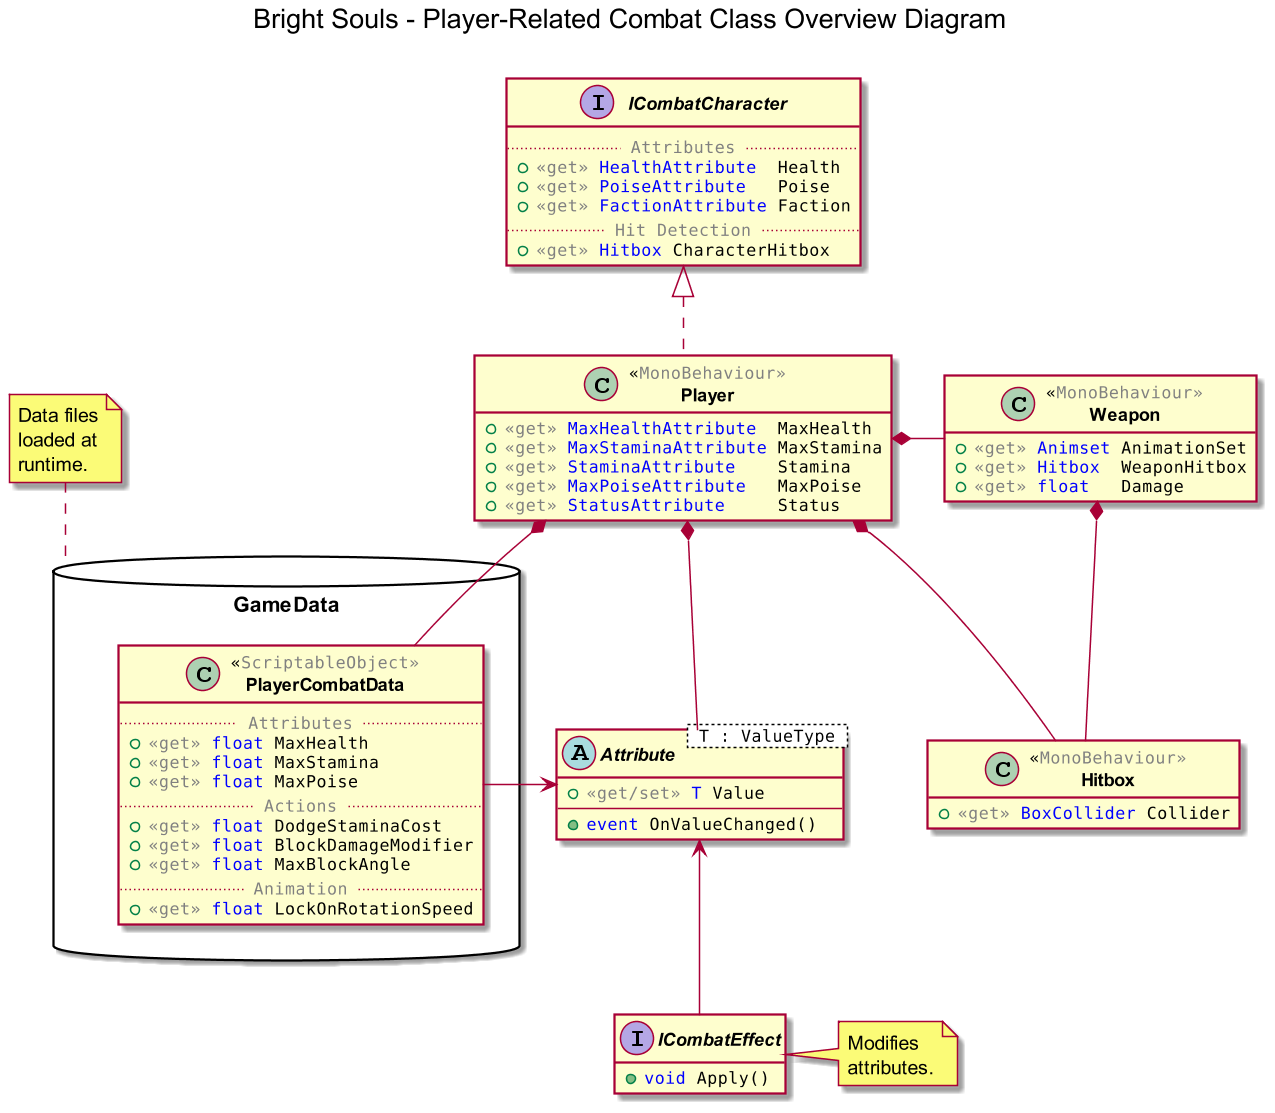
\includegraphics[width=34em]{figures/fig-combat-system-overview.png}
        \legend{Source: Diagram assembled by authors.}
    \end{center}
    \label{fig:combat-system-overview}
\end{figure}

% Attacking and combo system
%  - Continuously check for Attack input
We begin by listening to input from the player to determine when an \emph{Attack Command} should be issued. If the button mapped to the \emph{Attack Command} is pressed, we proceed to verify the current state of the player character to determine if an attack can be performed. The current state of the player is defined by a composition of boolean variables that reflect by the Animation being played on their character model.

% - Player/character is unable to perform attack if on Animation Lock
% - Attacks cost Stamina
If the character model is in the \emph{Dead}, \emph{Staggered}, \emph{AttackEnding}, \emph{On-Air}, \emph{Landing}, \emph{Dodging} or \emph{Blocking} animation states, the player is unable to perform an attack. This is commonly referred as \emph{Animation Locking} in games, and is an important aspect to potentially punish the player when taking strategically negative decisions. Attack Commands also have a resource cost for the player, where each attack depletes an amount of \emph{Stamina}. If the player Stamina resource has a value of zero, the player is unable to perform an attack. If the player has any Stamina value above zero, they are able to perform the attack.

%  - When sending attack command, enter a "combo" state and "Attack animation state machine"
%  - "OnCombo" state:
%    - Preemptively read player input before current attack animation ends. If player successfully sent attack input, continue the combo.
%    - If no attack input command is read within animation time frame, escape the Attack animation state machine
After an Attack Command is successfully validated, player state is set to \emph{Attacking} and the player enters an \emph{Attack State Machine} where Attack Commands are preemptively verified during attack animations. If an Attack Command is successfully executed before an attack animation ends an \emph{Attack Chain} is toggled, meaning that another attack animation is queued and transitioned to when the current attack animation ends. This behavior is commonly referred to as a \emph{Combo} in video games. Figure \ref{fig:player-anim-state-machine} shows the state machine definition that we use to implement the aforementioned behavior.

%     - Alternating between attack animations to create the impression of a seamless combo that is only limited by the stamina resource
This replicates how attacking works in Dark Souls, where the player can continuously enqueue attack commands until their \emph{Stamina} resource is depleted. If no Attack Command is successfully executed within the time frame of an attack animation, the player exits the \emph{Attack State Machine} and is locked to a short \emph{AttackEnding} animation state, where the player character model transitions from attacking to an idle state.

% Figure: Player Animation state machine
\begin{figure}[!ht]
    \caption{A state machine used for our implementation of the Attack and Combo system.}
    \vspace{0.5em}
    \begin{center}
        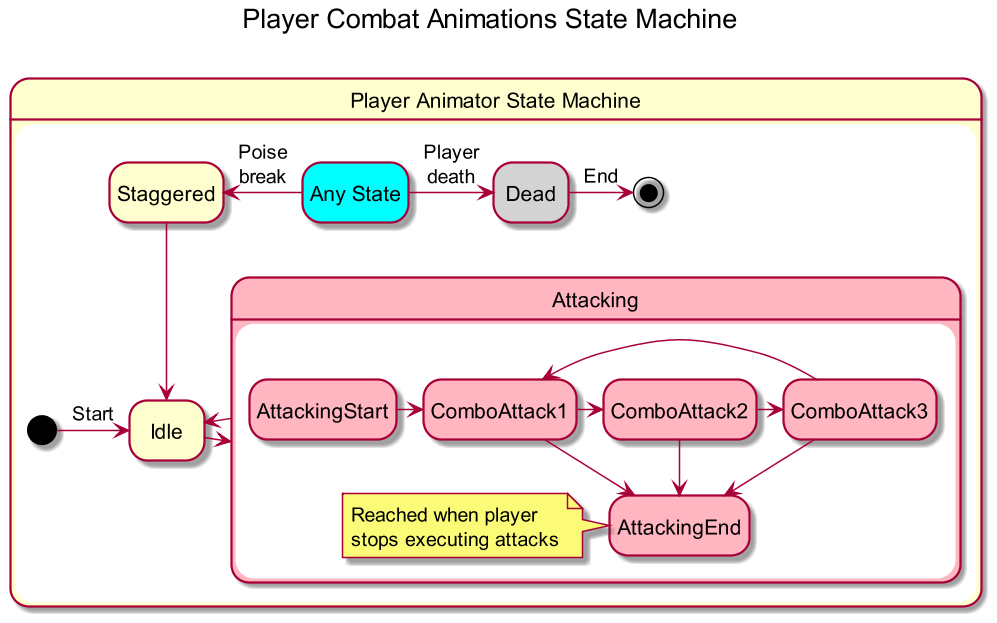
\includegraphics[width=34em]{figures/fig-player-anim-state-machine.png}
    \end{center}
    \legend{Source: Diagram assembled by authors.}
    \label{fig:player-anim-state-machine}
\end{figure}

%   > Hit detection toggled when receiving an event signal from the Attack animation
During Attack animations, the Animation System broadcasts event signals that toggle the activation and deactivation of the \emph{Hit Detection System}, which has the purpose of determining whether an attack successfully hit an enemy. At a certain point during the attack animation, we broadcast the \textsc{AttackCollisionStartEvent} which signalizes that attack collisions must be checked on each frame until an \textsc{AttackCollisionEndEvent} is signalized.

The \textsc{AttackCollisionEndEvent} is required to be signalized after the \textsc{AttackCollisionStartEvent} and before the attack animation ends so that attacks appropriately reflect what the attacking character performs. Generally, the point in time at which \textsc{AttackCollisionStartEvent} and \textsc{AttackCollisionEndEvent} are triggered should occur in the small time frame where the character swings the weapon in the direction of their target. Figure \ref{fig:attack-combo-diagram} shows the relationships between components involved in issuing Attack commands and handling combo states and animations.

% Figure: Attack and combos Class Diagram
\begin{figure}[!ht]
    \begin{center}
    \caption{A diagram showing the event flow and class relationship of the Attack and Combo related classes.}
    \vspace{0.5em}
        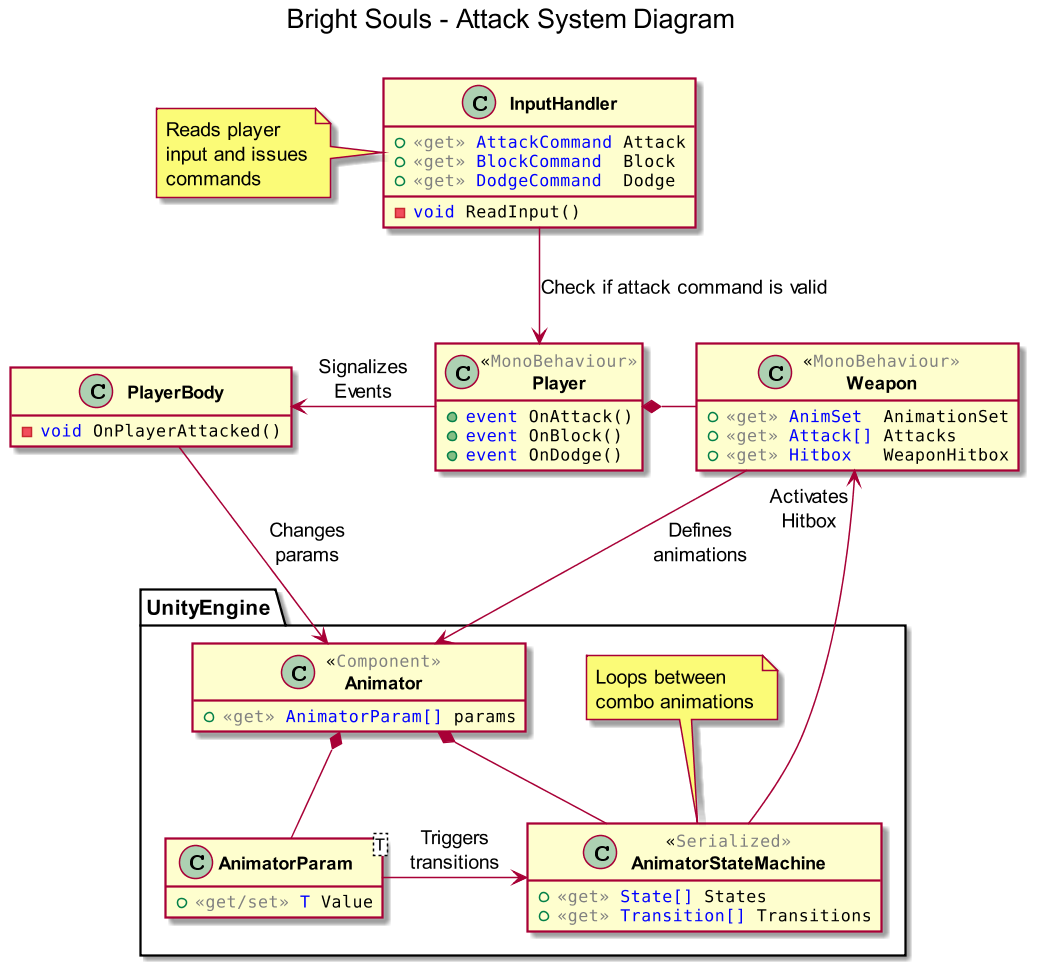
\includegraphics[width=34em]{figures/fig-attack-combo-diagram.png}
        \legend{Source: Diagram assembled by the authors.}
    \end{center}
    \label{fig:attack-combo-diagram}
\end{figure}

%     - Hit detection must not occur twice between the same target and same attack
%     - Specific collision layer to detect hitbox collision
To implement hit detection, we perform collider overlap checks in fixed time intervals of 16 milliseconds. These collision checks occur in a special collision layer called HitDetection, where every Collider is either the weapon of an attacker or the body of a target. This is an optimization requirement to meet the required time constraint in most computing systems. If a system is unable to meet the time constraint, there is a small chance that an attack might not be detected, where the attacker weapon "passes-by" the body of the attacker without triggering collision detection.

We estimate that attack collision detection occurs for approximately 20 frames from the point where it is first activated. Thus, if a computer system is able perform at least 4 updates per second, attack collision is guaranteed to be correctly detected. It is important to note that updates to the collision detection system are independent to the rendering performed by the graphics pipeline, and as a consequence are unaffected by most forms of temporary stutters in the application.

We also require safety measures to ensure that attack collision detection does not trigger a Hit event twice given the same Attack and Target entities. Therefore, for each attack performed by an attacking entity that is successfully registered as a Hit, we store a reference to an \emph{AttackCollision} instance in the \emph{Hitbox} component of the target entity. The Hitbox component then listens for the \emph{AttackCollisionEndEvent}, where the reference can be deleted since at this point the same \emph{AttackCollision} instance is not performing any collision checks.

% - Hit detection:
%   > Colliders:
%     - Hitbox overlap detection for attacker weapons and target character
%     - Attack Colliders are bounding boxes in weapons
%     - Character colliders are simplified bounding boxes that enclose torso, head and partially legs
For each occurrence of an attack collision, two colliders are obligatorily involved: one for the weapon of the attacker, and one for the body of the target. The colliders are instanced as \emph{bounding boxes}\sepfootnote{fn:bounding-boxes} that fully or partially enclose the 3D models of their relative entity. In order to perform collision checks with a reasonably optimized numbers of collision checks, we simplify bounding boxes of character models to only enclose the torso, head and a central position of the legs of a target. Using this method, we can minimize the amount of collision checks per frame, while also having appropriate precision for our implementation purposes.

%     - Consider character faction to recognize which combat characters can be hurt by an attack
After the collision detection step is performed, we must ensure that the attacking character is hitting a target that is not part of their own \emph{Combat Group} before validating an attack as a \emph{Successful Hit}. To do this we create the \textsc{FactionAttribute}, which determines that each character belongs to a combat group that is unable to perform attacks to other members of the same group. This is done so that groups of characters such as enemies of the player do not damage themselves when attempting to hit a target while being too close to each other. The values that the faction attribute can be assigned are described in table \ref{tab:table-faction-groups}. In addition, figure \ref{fig:hit-detection-diagram} shows the execution flow and class relationship of components used during the Hit Detection step.

% * Table: Values for the Faction Attribute
\begin{table}
    \begin{center}
      \caption{A description of the values that can be assigned to the \emph{Faction Attribute} of targets that are part of the Combat System in our implementation.}
      \label{tab:table-faction-groups}
      \rowcolors{2}{}{gray!25} % Alternate row colors
      \begin{tabular}{ >{\small}w{l}{3em} >{\small}w{c}{3em} m{25em} } % alignments and column size
        \addlinespace
        \toprule
        % Headings
        \bf Name    & \bf Id   & \bf Description                                              \\
        \midrule
        % 3D Models
        Player       &       0 & Player character. The player is a single entity and the sole 
                                 participant of this faction group.                           \\

        Enemy        &       1 & AI Agents that represent Enemies, which are hostile to the 
                                 player character.                                            \\

        NPC          &       2 & Non-Playable Characters. AI Agents which are not hostile to 
                                 the player character, but are hittable by and potentially 
                                 hostile to Enemies. An example of a Non-Playable Character 
                                 would be a companion which follows the player character and 
                                 aids them in combat encounters, being hostile to characters 
                                 belonging to the Enemy faction.                              \\

        Interactable &       3 & Static objects that can be attacked by the Player, Enemies or 
                                 Non-Player Characters and provide some type of feedback when 
                                 attacked. An example of an interactable entity would be a 
                                 barrel that can be attacked and destroyed.                   \\
        \bottomrule
      \end{tabular}
    \end{center}
\end{table}

% * Figure: Hit detection class diagram
\begin{figure}[!ht]
    \begin{center}
    \caption{Class diagram showing an overview of the components and flow of events related to the \emph{Hit Detection System}.}
    \vspace{0.5em}
        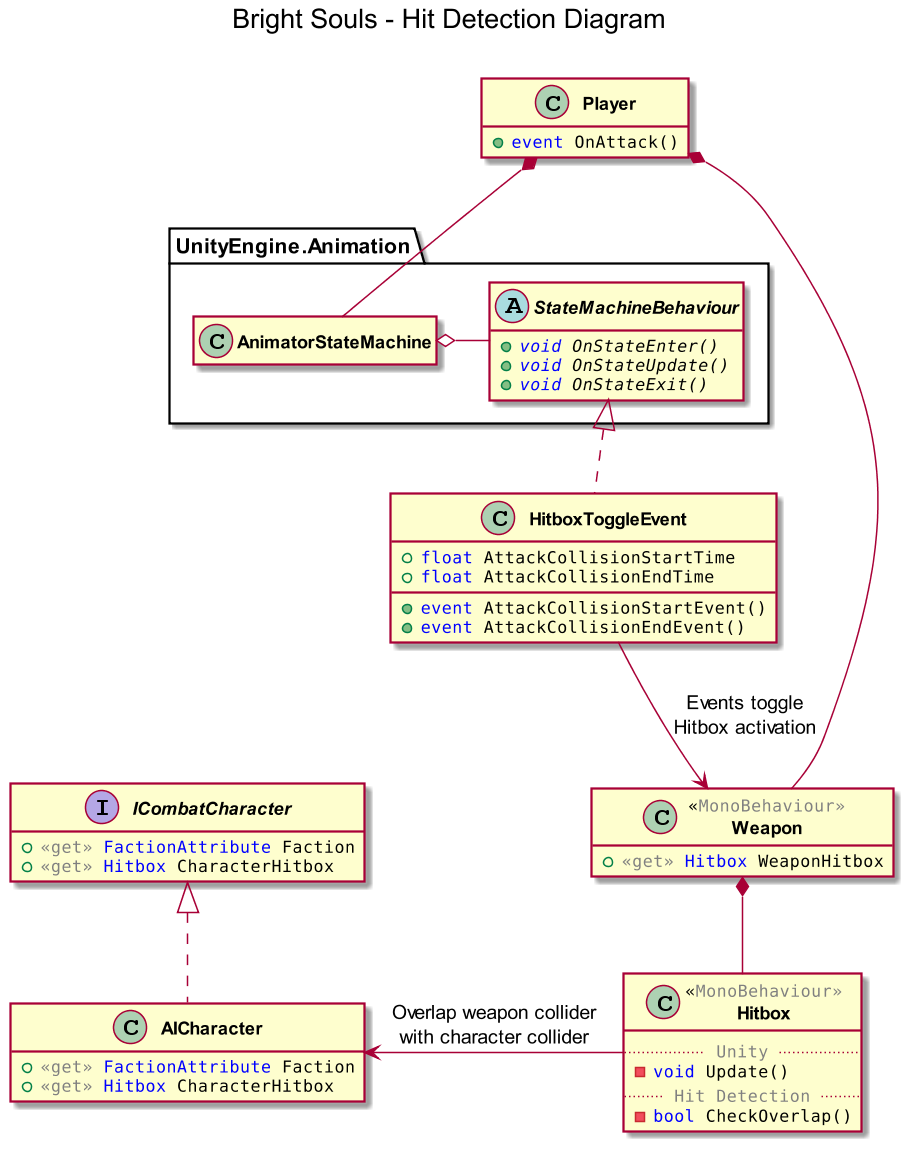
\includegraphics[width=30em]{figures/fig-hit-detection-diagram.png}
        \legend{Source: Diagram assembled by authors.}
    \end{center}
    \label{fig:hit-detection-diagram}
\end{figure}

% TODO Footnote fn:stagger
\sepfootnotecontent{fn:stagger}{Footnote: What is a stagger effect}

% TODO Footnote fn:knockback
\sepfootnotecontent{fn:knockback}{Footnote: What is a knockback effect}

% - Attack damage and other effects are abstracted into Combat effects
%     - Manipulate character attributes, statuses and physics
Once we performed all steps regarding the verification of whether an attack successfully hit an enemy, we can proceed to the next step of applying the \emph{Combat Effects} contained by the Attack. Combat Effects are our abstraction to the set of attribute effects, status effects and any other behaviors that occur when a character is struck by an attack. Examples of Combat Effects include the damage dealt to the Health of a target, Status effects such as \emph{Staggers}\sepfootnote{fn:stagger}, and physics effects such as the \emph{Knockback}\sepfootnote{fn:knockback} caused by an attack. Figure \ref{fig:combat-effects-diagram} shows an overview of the relationship between classes and components regarding the application of \textsc{CombatEffects} to \textsc{ICombatTarget} entities.

% * Figure: Combat Effect class diagram
\begin{figure}[!ht]
    \begin{center}
    \caption{Class diagram representing the relationships for Combat Effects and affected components.}
    \vspace{0.5em}
        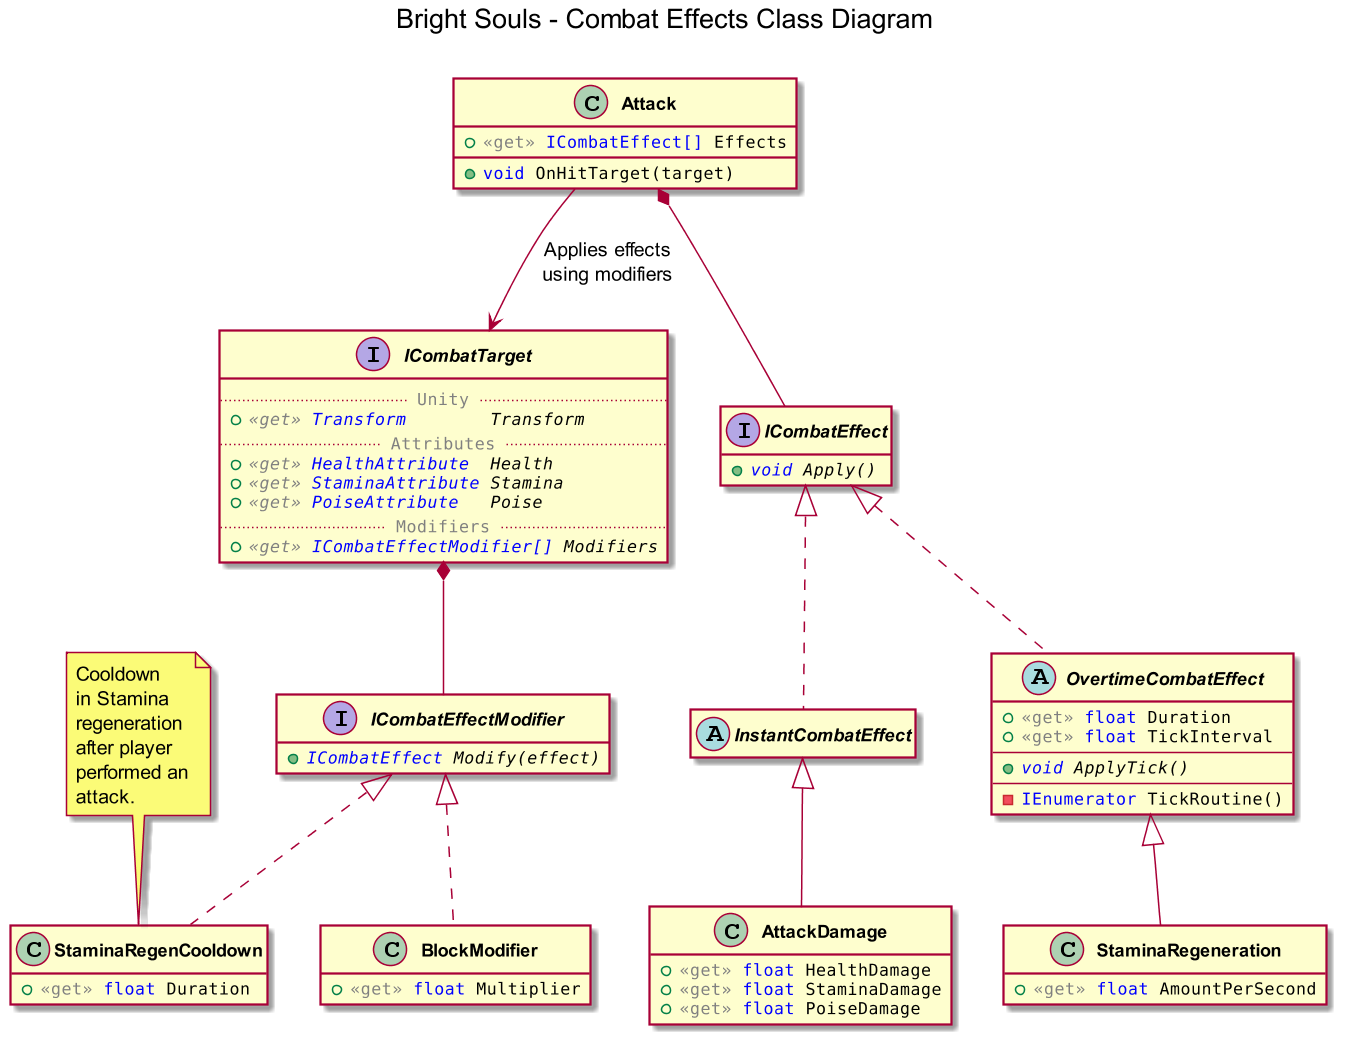
\includegraphics[width=32em]{figures/fig-combat-effects-diagram.png}
        \legend{Source: Diagram assembled by authors.}
        \label{fig:combat-effects-diagram}
    \end{center}
\end{figure}

%     - Instant combat effects are completely applied in the same frame as hit detection occurred
%     - Over-time combat effects with fixed interval ticks
In our implementation, we differentiate between \emph{Instant Combat Effects} and \emph{Over-time Combat Effects}. Instant Effects are applied to a target when a discrete event such as an attack takes place, and will often simply modify the value of an attribute. Examples of Instant Effects include the Health damage caused by an attack to a target and the Stamina cost of performing the attack, which is applied to the attacker. Over-time Effects are effects that occur in fixed time intervals over the course of a duration or is bound to the life of an entity.

% Player has a default Stamina regeneration effect
An example of Over-time effect would be the \textsc{StaminaRegeneration} effect that is permanently applied to the player, and which is temporarily blocked or modified by combat-related actions. During the course of a level, the player recovers a default amount of the Stamina resource over fixed time intervals, until either their Stamina resource is at the maximum possible amount or a combat action is performed. After a certain amount of time without issuing combat-related commands such as Attacking and Dodging, Stamina regeneration is re-enabled. Entering the Blocking state also modifies stamina regeneration by applying the \textsc{BlockingStaminaRegenModifier}, where the amount of stamina recovered is halved.

% - Combat Effect Modifiers
Combat Effects are restricted to performing modifications on a limited set of Attributes and Components exposed through the \textsc{ICombatTarget} interface, which is implemented by any entity that can be attacked. Before applying an effect to a target, we first check if the target contains any \emph{Combat Effect Modifiers}, such as a damage modifier caused by the target \emph{Blocking} or \emph{Dodging} an attack.

If the target has effect modifiers that are compatible with any of the effects being applied by an attack, the \textsc{Attack} class uses the modifiers to reconstruct its Combat Effects with updated values that reflect the purpose of the modifier. For instance, if the target successfully blocks an attack, the \textsc{BlockDamage} modifier is added to the target, which is used by the \textsc{Attack} class to update the \textsc{AttackDamage} combat effect by halving the damage that should be applied to the target. After the reconstruction of Combat Effects using any applicable modifiers, we finally commit to performing the attribute and status modifications and behaviors that are caused by an attack.

In figure \ref{fig:combat-flow-diagram}, we show an overview of all the steps involved with handling attacks, including detection of Attack commands being issued by the player, management of the animation states associated with weapons, validating Hitbox collision and combat groups with a Hit Detection System, and applying combat effects to modify target attributes and execute behaviors.

% * Figure: Flow of Combat System when processing Attack of entities
\begin{figure}[!ht]
    \begin{center}
    \caption{An event flow diagram that shows an overview of each step in our implementation of attacking in the Combat System.}
    \vspace{0.5em}
        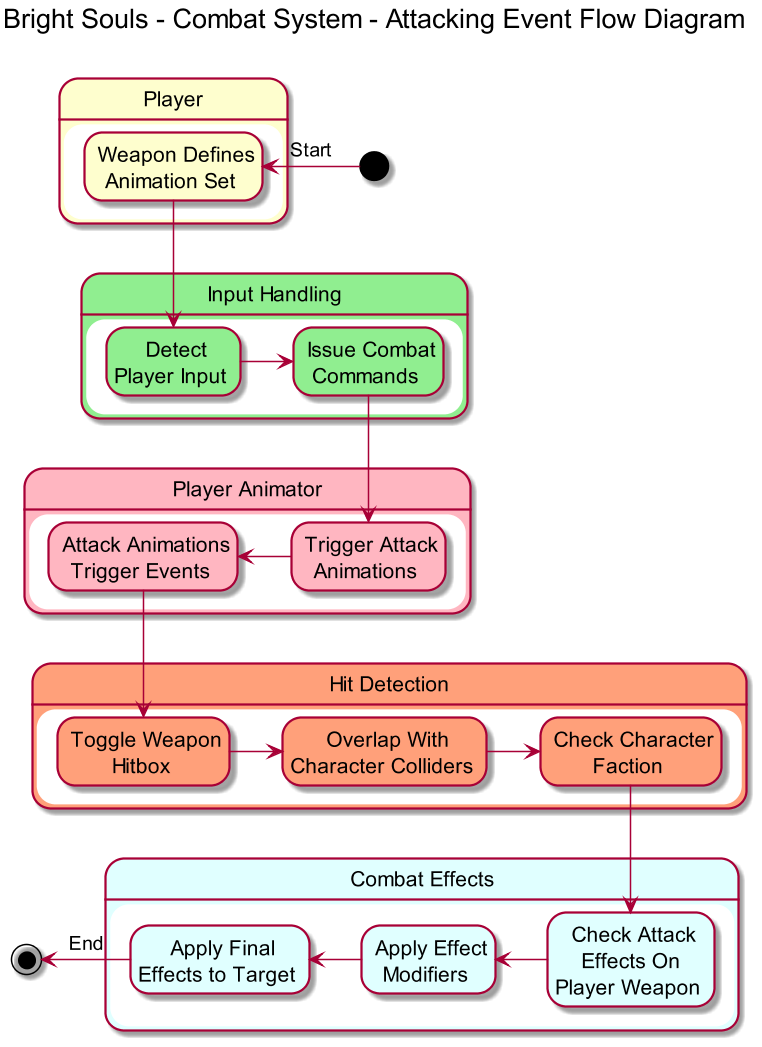
\includegraphics[width=22em]{figures/fig-combat-flow-diagram.png}
        \legend{Source: Diagram assembled by authors.}
    \end{center}
    \label{fig:combat-flow-diagram}
\end{figure}

%     - Block detection occurs when target is hit, is in "blocking" state and vector dot product between attack and target directions is < 0
To perform the blocking action, the player holds an input button which continuously issues the \textsc{BlockCommand}. When the player character is hit by an attack while performing the blocking action, we calculate the vector dot product between the attacker direction and the player direction before the player is hit. If the result has a negative value, it means that the player is pointing their shield towards the target, and thus it results in a successful block. If the target attacks the player from behind, the player is unable to block the attack.

% TODO (ADDITIONAL) Add formulae to vector dot product between defender and attacker direction, with outcomes.

%     - Dodge detection also occurs when target is hit. If hit detection occurs during target invincibility frames, a "dodge" is registered, and target receives no combat effects
Contrary to blocking, the \textsc{DodgeCommand} is issued discreetly at the press of a button. When the player presses the dodge command, the \textsc{Player} component signalizes the action to the animation system. If the player issues the command when moving towards a specific direction, the \textsc{Animator} component handles the movement of the \textsc{Transform} to translate the character into that direction. If the player is stationary when the dodge command is issued, the \textsc{Animator} simply uses the current direction defined by the \textsc{Transform}.

Over the duration of the dodge animation, we issue the \textsc{DodgeIFramesBegin} and the \textsc{DodgeIFramesEnd} events, which toggle the \textsc{Invincibility} combat effect modifier to the player. The Invincibility combat effect nullifies any negative combat effects that might affect the player during an attack, causing enemy attacks to have essentially no effect over the player.


% ============================================================================
% ============================================================================
% ============================================================================

% TODO \subsubsection{Animation System (ADDITIONAL)}

% Animation system
% - Difference in body movement when in Orbital vs Lock-On Cameras
% - React to attribute changes, motor velocity and physics updates

% - Figure: Player Animation State Machine

% - Statuses such as staggered, dead will override other animations
% - Blending between animations states when performing directional actions
% - Transitioning between combo states
% - Animation events for hit detection when attacking

% - Figure: Animation System class diagram showing component relations and events

% ============================================================================
% ============================================================================
% ============================================================================

\subsection{Artificial Intelligence and Enemy Design}

% TODO Footnote fn:cooldown
\sepfootnotecontent{fn:cooldown}{Footnote: What is a cooldown timer}

% Enemies in Dark Souls present basic, somewhat predictable behavior (REF Analysis Dark Souls)
As discussed in \ref{sec:analysis-dark-souls}, enemies in Dark Souls present basic and somewhat predictable behavior. When spawned, enemies either remain stationary or move through predefined paths until interaction with the player. When detecting player presence, they will often switch to a combat stance where they perform an attack from a limited and small set, and then switch to a defensive stance for the duration of a \emph{Cooldown}\sepfootnote{fn:cooldown} timer.

%   - Decided to use State Machines to replicate simplistic behavior
While we were unable to gather any specific information on how \emph{AI Agents} are implemented in the source code of Dark Souls, we argue that \emph{State Machines} can be used to implement the behaviors we observed and described. Using State Machines, we can represent the actions performed by enemies in Dark Souls as \emph{States} and \emph{Behaviors}. Each enemy will be in a particular State at a given point in time, and each State contains a set of behaviors that define the actions performed by an agent given environmental and player-related circumstances.

% ============================================================================
% ============================================================================
% ============================================================================

\subsubsection{State Machines}

To exemplify our claim, when an enemy is stationary we consider it to be in the \emph{Idle} state, which contains no particular Behaviors attached to it. When an enemy is moving along predefined paths and scouting for the player it is considered in the \emph{Patrolling} state, which contains the \emph{Scan} Behavior, which checks for the presence of the player in an area near the enemy, and the \emph{WaypointMovement} Behavior, which handles movement of the entity. Figure \ref{fig:fig-ai-state-machine} shows an example of a State Machine definition which is used by Melee-range enemies in our implementation, such as the \emph{Ghouls} and \emph{Warrior Skeletons}.

% * Figure: Melee enemy AI State Machine
\begin{figure}[!ht]
    \caption{An example of the State Machine that represents a Melee Enemy AI Agent. Each state holds its own behavior.}
    \begin{center}
        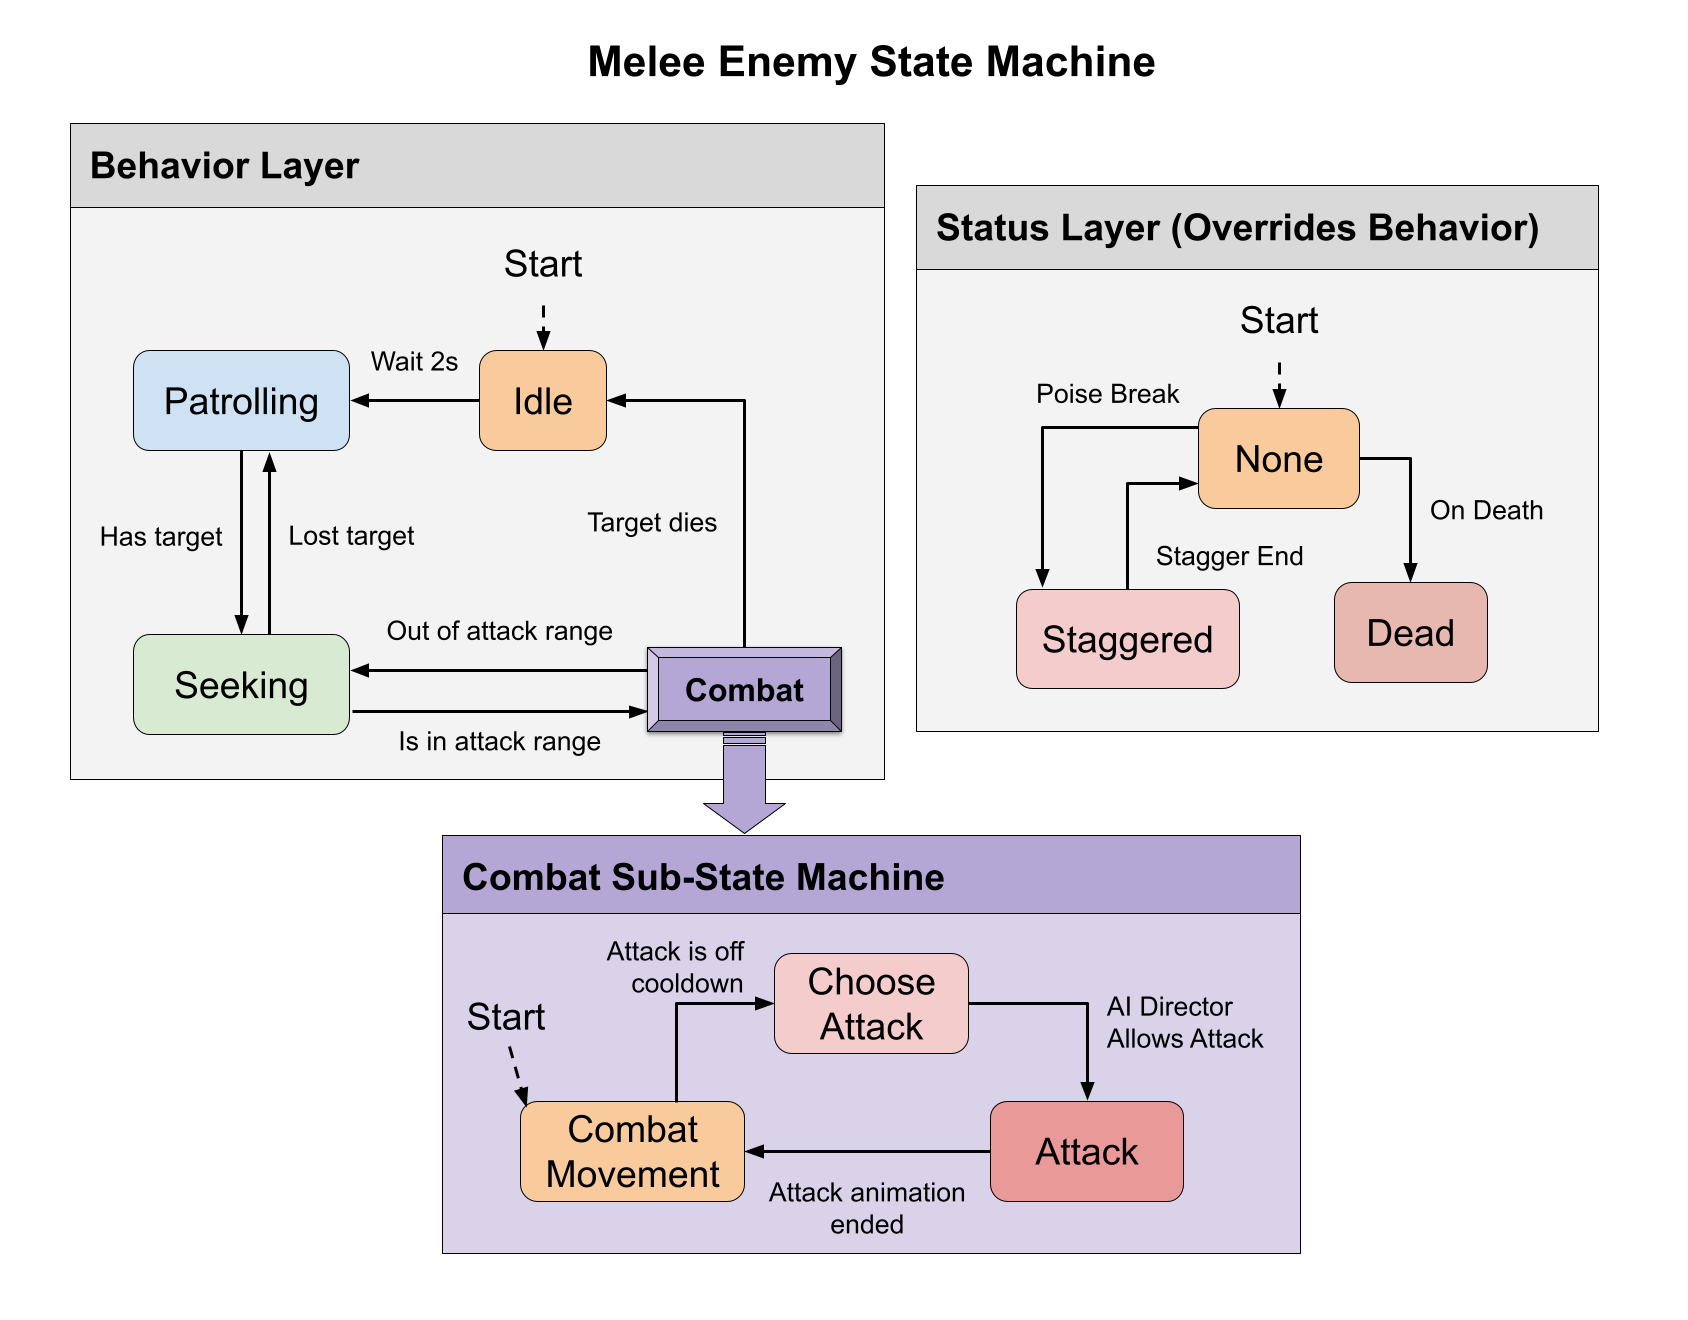
\includegraphics[width=34em]{figures/fig-melee-ai-state-machine.png}
    \end{center}
    \legend{Source: Diagram assembled by authors.}
    \label{fig:fig-ai-state-machine}
\end{figure}

% Implementation of a Serializable, multipurpose State Machine structure
%   - StateMachineController: MonoBehaviours, instanced in scenes. Contains a reference to the state machine and its owner. Validates conditions for transitions, performs transitions and updates states.
For our implementation, we use a generic definition of State Machines which can be used outside the scope of implementations of AI Agents. We start by defining a \textsc{StateMachineController} component which can be assigned to a MonoBehaviour. In the context of AI Agents, the StateMachineController will be attached to an \textsc{AICharacter} component, which represents the root hierarchy level of AI-controlled characters. The \textsc{StateMachineController} contains a reference to the \textsc{StateMachine} and to its owner, and is tasked with performing frame-bound updates to states and validating the conditions to perform transitions between states. Therefore, the \textsc{StateMachineController} is the sole runtime component in our State Machine implementation.

% - State Machines are bound to asset files
% - Class Definitions:States, Transitions, StateBehaviors
%   - StateMachine: Class definition for all the serialized data involving our implementation of state machines. Contains states and transitions. 
%   - States: Contain a variable set of Behaviors, that can be assigned dynamically during runtime and serialization.
%   - Transitions: References an origin and a target state, and contains a set of boolean conditions to validate a transition as valid.
The definitions of State Machine, including their States, Transitions and Behaviors are constrained to serializable space, with State Machines being bound to asset files that can be referenced to by the \textsc{StateMachineController}. The \textsc{StateMachine} class contains serialization data for \textsc{States}, which contain a variable set of \textsc{Behaviors}; and textsc{Transitions}, which contain references to an origin and target state and a set of boolean conditions to define when the transition should occur. Figure \ref{fig:state-machine-class-diagram} shows the class and data structure relationships for our implementation of state machines.

% * Figure: State Machine system architecture
\begin{figure}[!ht]
    \begin{center}
    \caption{Class relationship for our State Machine implementation from the perspective of AI Systems.}
    \vspace{0.5em}
        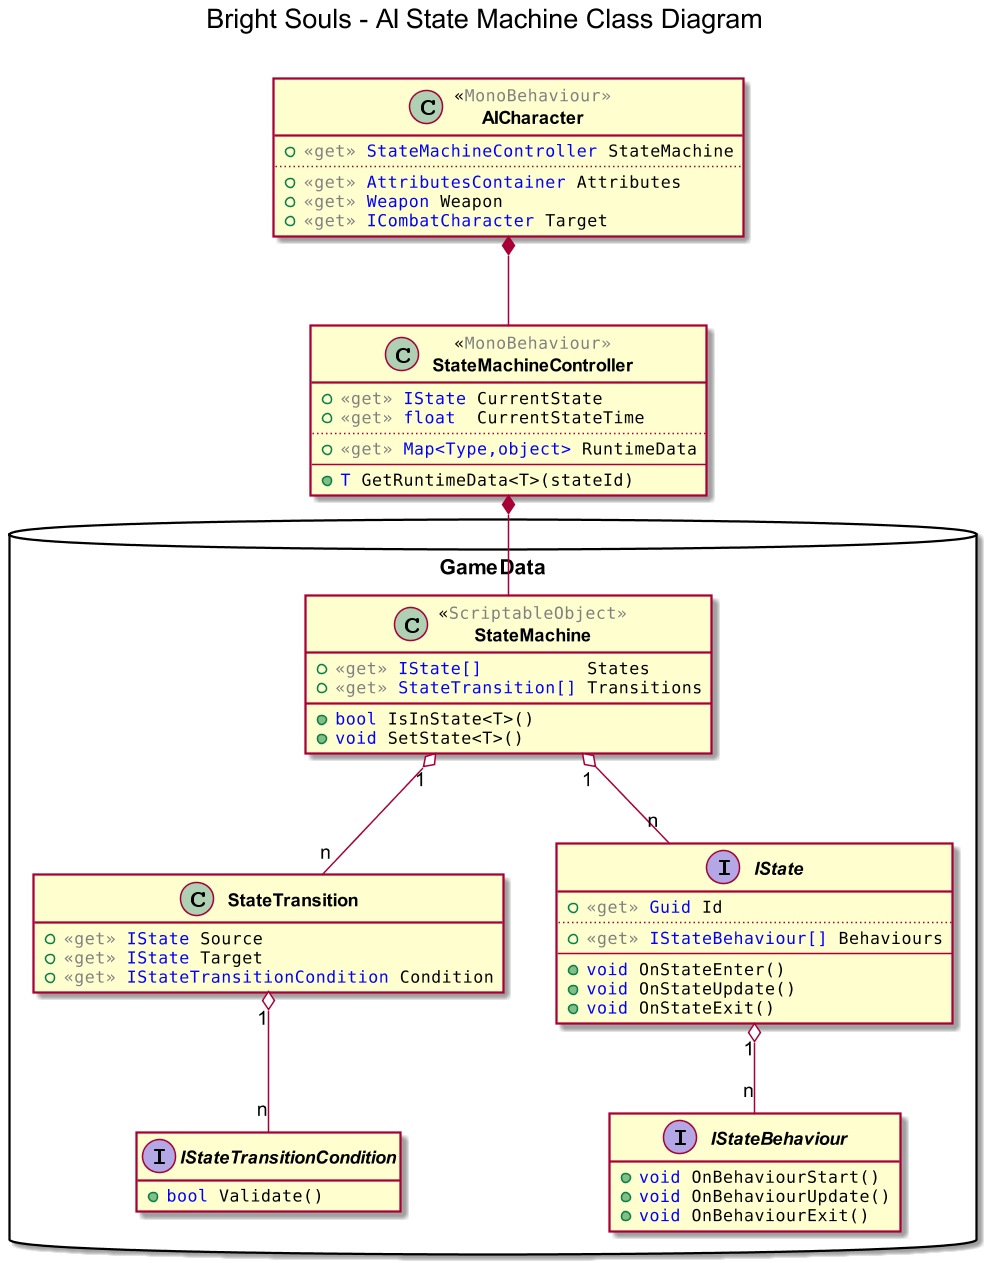
\includegraphics[width=28em]{figures/fig-state-machine-class-diagram.png}
        \legend{Source: Diagram assembled by authors.}
    \end{center}
    \label{fig:state-machine-class-diagram}
\end{figure}

% Each state has a set of dynamically assigned Behaviors that determine the actions performed by an AI Agent on that state.
Each \textsc{State} has a set of dynamically assignable \textsc{Behaviors}, which determine the actions that are performed by the AI Agent that contains the State Machine. In table \ref{tab:ai-behaviors}, we define all the possible behaviors in our implementation, specifying the States in which they are used and a brief description of the actions performed by the AI Agent when executing the Behavior.

% * Table - AICharacter Behaviors
% =================================================================================
% Name           | Related States   | Description
% =================================================================================
% WaypointMove   | Patrolling       | Uses a set of waypoints (which can be empty)
%                |                  | to move a character in fixed points on the
%                |                  | NavMesh of the environment.
% ---------------|------------------|----------------------------------------------
% Scan           | Idle, Patrolling | Uses a set of collision triggers to detect
%                |                  | enemies of the AI agent in an area around or
%                |                  | in front of its position, and assigns a 
%                |                  | target upon detection.
% ---------------|------------------|----------------------------------------------
% Seek           | Seeking          | Follows a target, constantly moving to its
%                |                  | position until the target is out of range.
% ---------------|------------------|----------------------------------------------
% AdjustDistance | CombatMovement   | Adjusts the distance of the AI Agent to be
%                |                  | close enough to perform an attack, without
%                |                  | being too close to the target.
% ---------------|------------------|----------------------------------------------
% PlanAttack     | CombatMovement   | Chooses the next attack based on the actions
%                |                  | being performed by the target, or by using
%                |                  | random number generation.
% ---------------|------------------|----------------------------------------------
% Attack         | CombatMovement   | Performs the chosen attack on the target
%                |                  | using the Attack System pipeline.
% ---------------|------------------|----------------------------------------------
% RotateAttack   | CombatMovement   | Performs body rotation to adjust the attack
%                |                  | to a moving target. The rotation has limited
%                |                  | speed to permit the target to dodge.
% ---------------|------------------|----------------------------------------------
% Shoot          | Shooting         | Used by ranged enemies. Continuously shoot
%                |                  | arrows at a target until the target is
%                |                  | out of range.
% ---------------|------------------|----------------------------------------------
% Death          | Dead             | Deactivates all components, triggers the
%                |                  | death animation and de-spawns the AI agent.
% =================================================================================

\begin{table}[!h]
    \begin{center}
      \caption{A list of the behaviors in the States of the AI Agents in our implementation.}
      \label{tab:ai-behaviors}
      \rowcolors{2}{}{gray!25} % Alternate row colors
      \begin{tabular}{ >{\small}w{l}{6em} >{\small}w{l}{7em} >{\small}m{17em} } % alignments and column size
        \addlinespace
        \toprule
        % Headings
        \bf Name       & \bf Related States  & \bf Description                              \\
        \midrule
        WaypointMove   & Patrolling          & Uses a set of waypoints (which can be empty)
                                               to move a character in fixed points on the 
                                               NavMesh of the environment.                  \\
        Scan           & Idle, Patrolling    & Uses a set of collision triggers to detect   
                                               enemies of the AI agent in an area around
                                               or in front of its position, and assigns a 
                                               target upon detection.                       \\
        Seek           & Seeking             & Follows a target, constantly moving to its
                                               position until the target is out of range.   \\
        AdjustDistance & CombatMovement      & Adjusts the distance of the AI Agent to be 
                                               close enough to perform an attack, without
                                               being too close to the target.               \\
        PlanAttack     & CombatMovement      & Chooses the next attack based on the actions 
                                               being performed by the target, or by using
                                               random number generation.                    \\
        Attack         & CombatMovement      & Performs the chosen attack on the target 
                                               using the Attack System pipeline.            \\
        RotateAttack   & CombatMovement      & Performs body rotation to adjust the attack 
                                               to a moving target. The rotation has limited 
                                               speed to permit the target to dodge.         \\
        Shoot          & Shooting            & Used by ranged enemies. Continuously shoot 
                                               arrows at a target until the target is 
                                               out of range.                                \\
        Death          & Dead                & Deactivates all components, triggers the 
                                               death animation and de-spawns the AI agent.  \\
        \bottomrule
      \end{tabular}
    \end{center}
  \end{table}

% State machines are serialized, therefore Behaviors are unable to keep state of objects that are instanced in a scene. We need to keep data for each behavior in the container of the state machine, which in this case is the AICharacter.
States are serialized and independent of any instanced objects, which in consequence creates the restriction that Behaviors are unable to store any type of runtime data from instanced entities, or even static data that is referenced by the entities. Therefore, we are required to maintain the data used by each behavior in the container of the \textsc{StateMachineController}. For this reason we create the \textsc{IStateMachineOwner} interface, which provides a public accessor to a \textsc{Hashmap} structure which contains the runtime and referenced data for an instanced entity, using an identifier for the current state as the \emph{Key}.

% ============================================================================
% ============================================================================
% ============================================================================

\subsubsection{Implementation of Behaviors}

% Movement:
%   - Use of NavMeshes to define walkable space in 3D environment for AI Agents.
%   - Use of A* path-finding algorithm to define movement over nodes scattered throughout the mesh.
For an AI Agent to perform movement over the environments that were assembled when executing the \textsc{WaypointMove} or \textsc{Seek} behaviors we use Unity's \emph{NavMesh} system, which uses the topology of 3D objects and a user-defined set of layers with movement costs to generate a simplified mesh representing the traversable ground in the environment. The resulting mesh also contains weights for each vertex, which causes the AI Agent to prioritize certain paths defined by the user. Using the data generated from \emph{NavMeshes}, we define the movement performed by the AI as a set of waypoints that are calculated using the \textsc{A*} algorithm with the \textsc{Manhattan Distance} heuristic.

% TODO Footnote fn:forward-vector
\sepfootnotecontent{fn:forward-vector}{Footnote: What is the forward vector}

% How AI agents scan for targets
% - Spheric collider for frontal view cone
%      - Detects collision with ICombatCharacters from different Faction
% - Calculate the angle between agent forward and target relative pos
To scan for targets in the environment, AI Agents have a spheric collider representing the radius where a target can be detected by a frontal view cone. The collider detects collision with \textsc{ICombatCharacter} entities where the \textsc{FactionAttribute} has a different value to that of the agent. If a target is within this radius, we calculate the angle between the forward vector\sepfootnote{fn:forward-vector} of the agent and the relative direction of the target. The forward vector is natively supplied by \textsc{Unity} with the \textsc{Transform} component, but we also need to project the vector onto the two-dimensional [X, Z] plane.

% - How target relative pos is calculated
% - Use of another, smaller spheric collider for enemy hearing
The \emph{Target Relative Direction} is calculated by subtracting the target position to the position of the agent, normalizing the result and projecting it onto the ground plane. Having these vectors, we use the \textsc{Vector3.Angle} operation from \textsc{Unity} to clamp field detection range to a cone of 90 degrees, causing the agent to have a constrained field of view. Additionally, we use another spheric collider with smaller radius to represent the distance in which the AI Agent would be able to hear. When an entity of the type \textsc{ICombatCharacter} enters this collider, the AI Agent will immediately consider it as the new target.

% - What happens when the target dies
%       - AI agent is reset to Idle
% - If target is unreachable, same thing happens
When the target dies, the AI agent is reset to their default state - which is generally the start point of its state machine. Therefore, when an enemy AI agent is able to defeat the player, they will return to the \emph{Idle} state. A similar event happens when the AI agent is in the \emph{Seeking} state and the target can not be interacted with. If the target is in an unreachable position where there is no path connecting the ground NavMesh from agent to player position, the AI loses interest in the target and returns to its default state.

% How AI Agents attack
%   - Each enemy has own state machine
%   - State state differs because of behaviors and data
%   - CombatMovement: adjust position, plan attack, execute
In our implementation, we group AI agents by an \emph{Enemy Type}. Each enemy type will have its own State Machine definition. While the State Machine for an enemy type might contain states with the same name as another, their functionality differs by using a different set of behaviors or different values for the data in the behaviors. The most relevant example would be in the \textsc{CombatMovement} state where a melee AI agent must adjust their position, plan their attack and perform the attack based on their position in the environment, their available actions and the actions being performed by the player. The \textsc{CombatMovement} state is functionally the same as the sub-state machine concept used in hierarchical state machines. We switch between three unique behaviors to give the impression of different states: \emph{PositionAdjustment}, \emph{AttackPlanning} and \emph{AttackExecution}.

% AdjustPosition
%     - Two-dimensional radial and distance-based positioning
In the \textsc{PositionAdjustment} behavior, we have several steps to calculate the position an AI agent should move towards. We start by defining a two-dimensional vector to define the position an AI agent should be in relative to their target: a \emph{distance relationship} between the agent and their target and a \emph{radial-distribution} position, where the agent positions itself in a circular perimeter around the target.

%     - GroupAIBrain: What is the expected distance?
To define the distance relationship between the agent and their target, we consider parameters that define the context of the combat encounter. First, we communicate with the \textsc{GroupAIBrain} component to understand whether the player is dealing with too many enemies, which means the agent should take a more idle stance and remain in the backline. The \textsc{GroupAIBrain} component is a manager to all AI agents engaged in a \emph{Combat Encounter} against the player. Specific details about functionality involving the \textsc{GroupAIBrain} component will be further discussed in section \ref{sec:ai-brain}.

\sepfootnotecontent{fn:hitbox-central-point}{Footnote: What is the hitbox central point?}

%     - Is the attack in cooldown?
%     - Distance to Player: Would an attack hit?
Second, we determine if the AI agent attacks are on \emph{cooldown}, meaning that the agent is not able to attack for a short period of time after performing another attack. If so, the agent takes a defensive approach and attempts to position itself further away from the player so that the player has to make a time investment to be able to attack the agent. Third, we calculate the average \emph{Hitbox Central Point}\sepfootnote{fn:hitbox-central-point} distance for all attacks that the AI Agent can perform. We use this average to create a target position that minimizes the chances of the player being able to avoid an attack by simply moving backwards. This step is performed when the target is either out of attack range or after half of the \emph{cooldown} duration for the next attack.

% - GroupAIBrain: What is the expected radial position?
%     - Priority index
%     - Positions in arc in circular perimeter
%     - Arc boundaries restricted by environment geometry
%     - Arc also restricted by dynamic radian in GroupAIBrain
To define the radial-distribution position for an entity, the AI Agent is assigned a numeric priority index upon entering a \emph{Combat Encounter} instance against the player. The value of the priority index is used to evenly arrange AI Agents in a constrained arc of a circular perimeter around the player. The aperture of the arc is defined by both the geometry of environment colliders around the player and adjustment metrics. If the arc boundaries are not restricted by environmental geometry, the aperture is defined by an adjustable radian supplied by the \textsc{GroupAIBrain} component.

% - How agents are distributed in the arc
% - Arc divided in equal size segment
% - First agent in center
% - Second and third agent in boundaries
The agent placement arc is divided in equal size segments that are used to distribute the agents uniformly in relation to the player. At the beginning of a combat encounter, a single agent becomes part of the AI group. This initial agent is defined as the pivot for the group. The arc is divided in two segments by the position of the pivot agent, which is exactly at the center of the two segments. The following two agents are placed at the outer boundaries of the arc, each at the limits of their respective segments.

% - Subsequent agents subdivides largest segments from center outwards
% - Recalculate segments when agents die
Every subsequent agent subdivides the largest segment that is closest to the pivot, using the center position of the segment and creating two new segments. When the pivot agent is defeated, a new pivot agent is selected based on its distance from the original pivot, and the segments are recalculated by adding each subsequent agent that is closest to the pivot through the same algorithm. When non-pivot agents are defeated, the group is also recalculated but with the difference that we use the same pivot when recalculating agent segments. This algorithm is exemplified by figure \ref{fig:arc-segments}, and the resulting behavior can be seen in figure \ref{fig:enemy-positioning-example}.

% * Figure: Figure illustrating the behavior of the "arc segments" algorithm
\begin{figure}[!ht]
    \caption{Illustration of the "Arc Segments" algorithm for radial positioning of AI Agents around the player character.}
    \begin{center}
        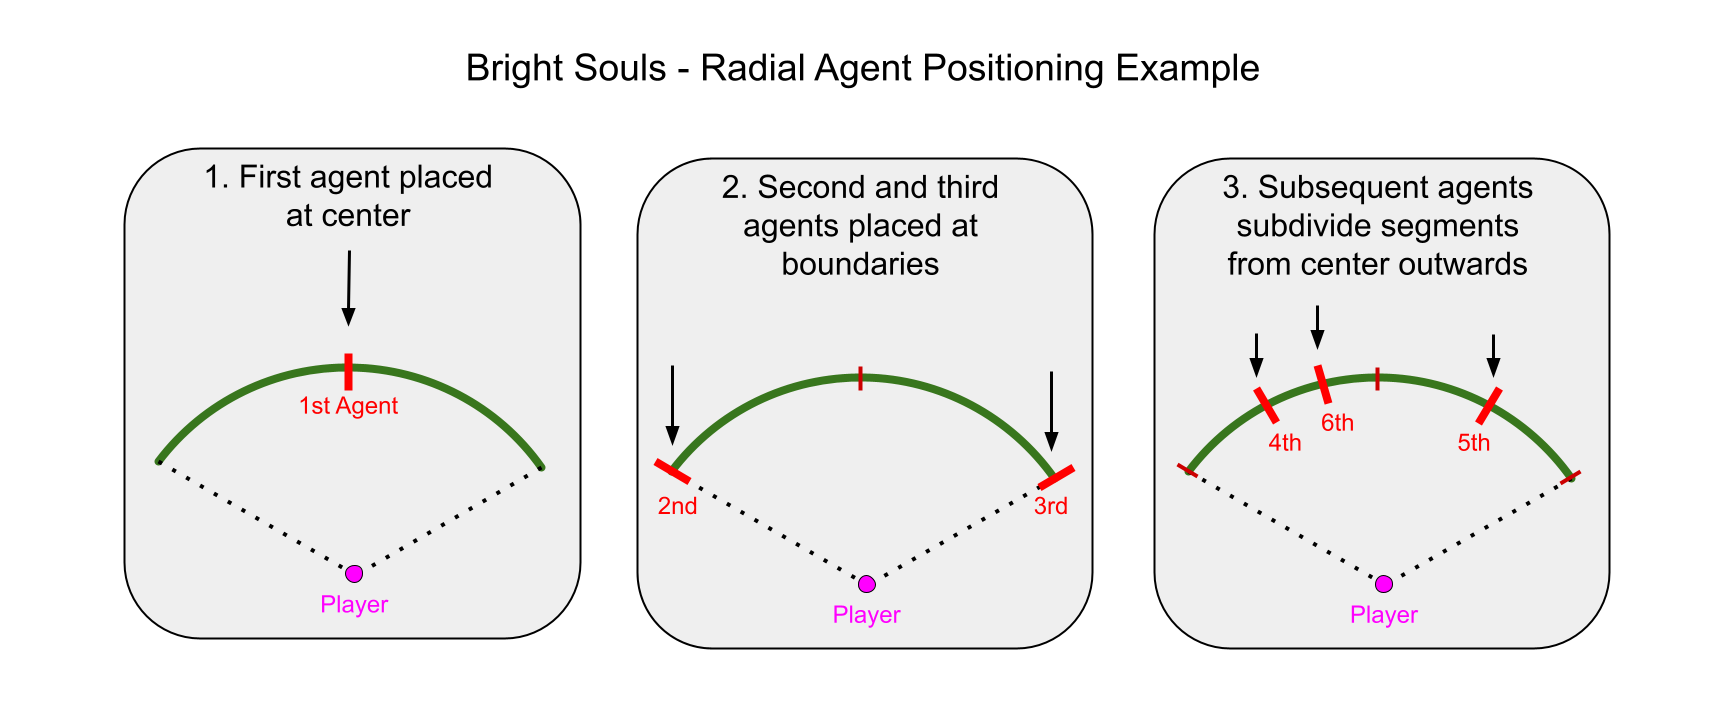
\includegraphics[width=32em]{figures/fig-arc-segments.png}
    \end{center}
    \legend{Source: Diagram assembled by authors.}
    \label{fig:arc-segments}
\end{figure}

% * Figure: Enemy typical radial placement around the player character
\begin{figure}[!ht]
    \caption{An example of melee enemy group positioning with five AI Agent enemies.}
    \begin{center}
        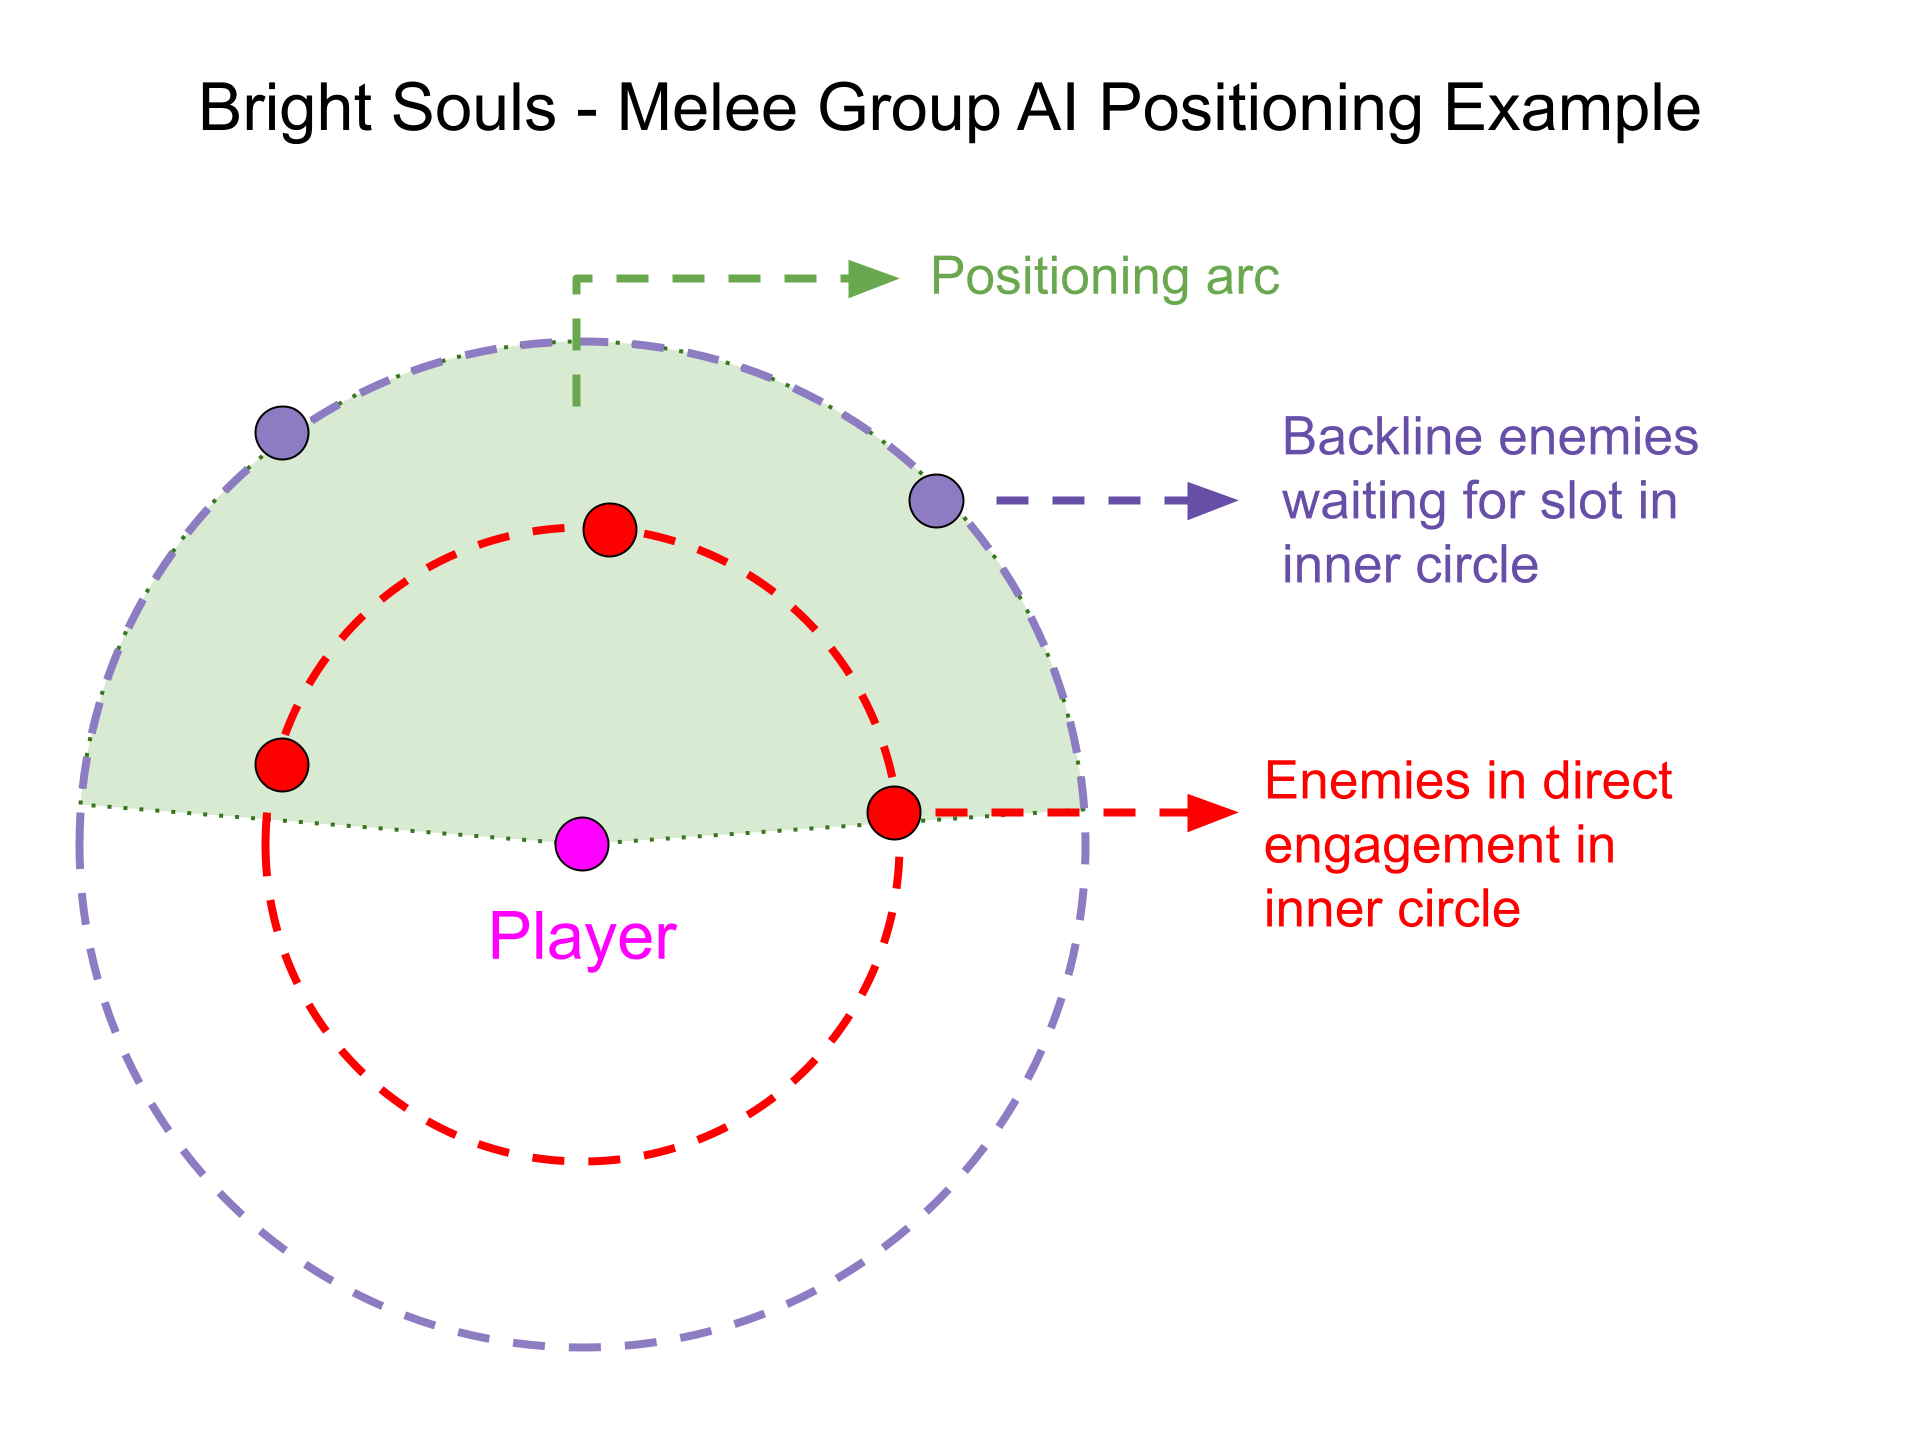
\includegraphics[width=26em]{figures/fig-enemy-positioning-example.png}
    \end{center}
    \legend{Source: Diagram assembled by authors.}
    \label{fig:enemy-positioning-example}
\end{figure}

% PlanAttack behavior
% Player State + GroupAIBrain info used as input
% Decide if can attack and which attack
In the \textsc{PlanAttack} behavior, we use information from player state along with constraints imposed by the \textsc{GroupAIBrain} component to define if an attack can be executed, and which attack the AI Agent should perform at a given context. Each attack has a different purpose designed to guide the player towards a specific response. In table \ref{tab:enemy-attack-types} we present the implemented attack types and the entities that are able to use it.

% TODO Footnote fn:poise-break
\sepfootnotecontent{fn:poise-break}{Footnote: What is Poise Break}

%     - AI Brain: Does it give permission to attack?
%     - EGCD: Enemy Group Cool-Down
First, we query the \textsc{GroupAIBrain} component to check whether the current AI Agent being processed has permission to attack. Enemy AI Groups have a shared set of \emph{Enemy Group Cooldown} timers that are reset every time an AI agent performs an attack. All AI Agents that are part of a group will be unable to attack unless at least one of the available cooldown timers has a specific amount of elapsed time. Both the numbers of timers available and the minimum elapsed time for each are determined by adaptive parameters from the \textsc{GroupAIBrain} component, and are further discussed in section \ref{sec:adjustments}.

% Uses list of available types to query for information
%     - AI Brain: does it give permission for special attack?
Second, the PlanAttack behavior uses information on the available attack types to query which information is necessary to decide the attack. We communicate with the \textsc{GroupAIBrain} component to determine if the entity is able to perform \emph{Special Attacks}. Given a small interval of time, a limited number of non-basic attacks can be performed by an agent. If the agent is unable to perform a Special Attack after querying availability from the \textsc{GroupAIBrain} component, it simply chooses one of multiple basic attacks to perform.

Non-basic attacks have the purpose of creating incentive for the player to perform a new or specific reaction. For instance, the \emph{Overhead} and \emph{Pierce} attacks are designed to punish the player if attempted to be blocked and drain their Stamina resource. If the player does attempt to block one of such attacks, they will quickly find themselves out of Stamina and trigger a \emph{Poise Break}\sepfootnote{fn:poise-break}.

%     - Is the player out of attack range?
%     - How often does the player back-step
Then, we check if the player is still out of attack range even after the adjusting its position during the PositionAdjustment behavior. If so, we use a parametrized threshold related to the chance of an agent performing a \emph{Charge} attack, if it is one the available movements. The threshold is combined with a \emph{profile} metric regarding the frequency the player uses back-steps to avoid attacks, and then used as input for a RNG (random number generation) algorithm to determine if the agent will perform the \emph{Charge} attack. The parametrized thresholds for each attack type are explained further in section \ref{sec:adjustments}. If the agent is not able to perform the \emph{Charge} attack, it is reverted back to the \emph{PositionAdjustment} behavior.

%         - Is the player blocking?
%         - How often does the player block, dodge?
In the same sense, we check if the player is blocking and use a threshold related to the chance of the agent performing an \emph{Anti-Block} attack, such as the \emph{Overhead} or \emph{Pierce} attacks. We combine that chance with the player \emph{profile} metric regarding the frequency which the player uses the Block Action to mitigate the damage of attacks, and use these values as input for the RNG algorithm to determine if the agent will perform an \emph{Anti-Block} attack. Anti-dodge attacks use a similar threshold adjustment system, with the exception that it is not considered whether the player is performing a dodge or not. Since the dodging action is discrete and occurs in a fraction of a second, the agent has to be able to predict when a player would perform a dodge so that the attack punishes the player.

% ============================================================================
% ============================================================================
% ============================================================================

% TODO \subsubsection{Management of Agent Groups}
%\label{sec:ai-brain}

% ============================================================================
% ============================================================================
% ============================================================================

% TODO \subsection{Design of Enemy Types (ADDITIONAL)}

% TODO Table - Enemy Types
%
% =========|============|========|===========|=========|==========================================
%  Name    | Move Speed | Damage | Atk Speed | Health  | Description                             
% =========|============|========|===========|=========|==========================================
% Ghoul    | Slowest    | Lowest | Slow      | Lowest  | Slow and weak enemy. Introductory enemy 
%          |            |        |           |         | for player to test mechanics.
% ---------|------------|--------|-----------|---------|------------------------------------------
% Skeleton | Fast       | Low    | Medium    | Low     | Fast enemy. Causes player to reposition 
%          |            |        |           |         | and protects archers.                  
% ---------|------------|--------|-----------|---------|------------------------------------------
% Warrior  | Slow       | Medium | Slowest   | High    | Uses shield. Hard to kill. Buys time for  
%          |            |        |           |         | all other enemies.  
% ---------|------------|--------|-----------|---------|------------------------------------------ 
% Archer   | Stationary | Low    | Slowest   | Medium  | Meant to slowly drain player health from
%          |            |        |           |         | a distance if not prioritized.           
% ---------|------------|--------|-----------|---------|------------------------------------------
% Knight   | Medium     | High   | Fast      | Highest | Meant to force player to dodge, blocking 
%          |            |        |           |         | his Attacks Drain too much Stamina.      
% =========|============|========|===========|=========|==========================================

% TODO Table - Attack Speed Values (tab:attack-speed-values)
%
% ==========|======|===========
% Atk Speed | APS  | Entities
% ==========|======|===========
% Slowest   | 0.33 | Archers,
%           |      | Warriors
% ----------|------|-----------
% Slow      |  0.5 | Ghouls
% ----------|------|-----------
% Medium    |  0.8 | Skeletons
% ----------|------|-----------
% Fast      |  1.5 | Knights
% ----------|------|-----------
% Fastest   |  2.3 | Player
% ==========|======|===========

% TODO Table - Health Values (tab:enemy-health-values)
%
% ========|======|===========
% Health  | PATK | Entities
% ========|======|===========
% Lowest  |    2 | Ghouls
% --------|------|-----------
% Low     |    3 | Skeletons
% --------|------|-----------
% Medium  |    6 | Archers
% --------|------|-----------
% High    |    8 | Warriors
% --------|------|-----------
% Highest |   10 | Knights
% ========|======|===========

% TODO Table - Damage Values (tab:enemy-damage-values)
%
% =======|======|===========
% Damage | ATKP | Entities
% =======|======|===========
% Lowest |   20 | Ghouls
% -------|------|-----------
% Low    |   14 | Archers, 
%        |      | Skeletons
% -------|------|-----------
% Medium |   12 | Warriors
% -------|------|-----------
% High   |    9 | Knights
% =======|======|===========

% TODO Table - Attack Types (tab:enemy-attack-types)
%
% =========|============|==========|===============================
% Name     | Type       | Enemies  | Description
% =========|============|==========|===============================
% Slash    | Basic      | Ghoul,   | Low damage attack, no health
%          |            | Skeleton | damage when blocked. Low poise
%          |            |          | damage.
% ---------|------------|----------|-------------------------------
% Arrow    | Basic      | Archer   | Low damage attack, no damage
%          |            |          | when blocked.
% ---------|------------|----------|-------------------------------
% Double   | Basic      | Knight   | Medium damage attacks, low 
% Slash    |            |          | damage when blocked.
% ---------|------------|----------|-------------------------------
% Charge   | Gap Closer | Skeleton,| Medium damage attack. Enemy
%          |            | Knight   | runs to player to land the
%          |            |          | attack from a long distance.
% ---------|------------|----------|-------------------------------
% Overhead | Anti-Block | Warrior  | Medium damage attack. Consumes
%          |            |          | half of player stamina if
%          |            |          | attempted to be blocked.
% ---------|------------|----------|-------------------------------
% Pierce   | Anti-Block | Knight   | High damage attack. Pierces
%          |            |          | through player defense, 
%          |            |          | consuming most of player
%          |            |          | stamina if blocked.
% ---------|------------|----------|-------------------------------
% Sweep    | Anti-Dodge | Knight   | Medium damage attack. Has
%          |            |          | three hit detection phases
%          |            |          | and a long duration. Meant
%          |            |          | to catch the player in the
%          |            |          | final position after a dodge.
% =========|============|==========|===============================

% ============================================================================
% ============================================================================
% ============================================================================

% TODO \subsection{Level Design (ADDITIONAL)}

% ============================================================================
% ============================================================================
% ============================================================================

% TODO \subsection{Audio and Visual Effects (ADDITIONAL)}

% ============================================================================
% ============================================================================
% ============================================================================

% TODO \subsection{User Interface (ADDITIONAL)}

% ============================================================================
% ============================================================================
% ============================================================================

\subsection{Telemetry and Performance Tracking (WIP)}

To perform difficulty adjustments that satisfy the skill level and knowledge of a player regarding our implementation, we need to capture data regarding to how the game is being played. We then must use the data to reconstruct an order of events and analyze the patterns and outcomes of player actions, to determine if the player is being overtly successful or failing to meet the requirements of the challenged that was imposed by the current difficulty.

We can start to determine the player \emph{profile} and \emph{performance} by implementing a pipeline of data acquisition, manipulation and analysis using a log of \emph{Events} raised during a play session. To do this, we implement a set of components that observe the actions performed by in-game entities to raise parametrized events while also gathering variable elements of contextual data as input.

Events are then packaged into a standardized data structure called \textsc{EventInstance}, where we store data such as a \emph{Timestamp} which represents the time since application start where an event was raised, a \emph{Name} which is used as an identifier for the event, a \emph{Type} which is used to determine the superset of systems where the event is raised, a \emph{Source} which is used to determine which in-game entity the event is related to, and a set of \emph{Parameters} which are valued types that might contain contextual data for the event. Table \ref{tab:event-instance} shows a detailed description of the fields in the \textsc{EventInstance} data structure, along with the associated types for each fields.

% * Table: Event Instances
% Event Instance
%   • Timestamp ( Time : double )
%   • Name ( String )
%   • Type ( String )
%   • Source ( ObjectId : GUID )
%   • Params[]
%       • { "name", "type", "value" }

\begin{table}
    \begin{center}
      \caption{A description of the fields associated with an \textsc{EventInstance}.}
      \label{tab:event-instance}
      \rowcolors{2}{}{gray!25} % Alternate row colors
      \begin{tabular}{ >{\small}w{l}{5em} m{7em} m{16em} } % alignments and column size
        \addlinespace
        \toprule
        % Headings
        \bf Field Name & \bf Field Type  & \bf Description \\
        \midrule
        % Data
        Timestamp      & double          & The time since application start when an event was 
                                           raised. Measured in seconds.                        \\
        Name           & String          & The Name Identifier for an event.                   \\
        Type           & String          & The System from which the event is raised from.     \\
        Source         & ObjectId        & The source in-game entity which caused the event to 
                                           be raised.                                          \\
        Params         & Array of Tuples & A set of data parameters, given in string format,  
                                           that are used to represent any contextual related 
                                           with the event.                                     \\
        \bottomrule
      \end{tabular}
    \end{center}
\end{table}

% - Write events to file in batches for performance
Events are captured and written to output files in batches to minimize performance costs over extended gameplay sessions. By doing this, frame rendering "hiccups" are minimized to a few particular moments where events exceed a specific threshold of allocated memory for batches, and in most instances do not occur over the duration of a game level. We attempt to keep the use of the input/output system and any data processing restricted to the duration of the loading screen, which happens in the transition between in-game levels. Since players does not have any sort of input or control over the application during the loading screen, this implementation abstracts the processing from the player, keeping the gameplay experience fluid.

\sepfootnotecontent{fn:play-session}{A Play Session is delimited by the moment where a user starts the game application and the moment where the user exits the application, returning to the operating system.}

% - Events are stored in a simple .csv file
% - .csv file is uploaded to google sheets after session
For each \emph{Play Session}\sepfootnote{fn:play-session}, we store a unique \emph{CSV} (Comma-Separated Values) file that is implemented to serve as a simplified relational database to store in-game events. Before the end of a play session and after all levels are completed by the player, our database file is uploaded to a \emph{Google Sheets} repository using the Sheets API.

\subsubsection{Captured Events}

In this section, we specify the basic events that are captured in the data acquisition step of our performance tracking pipeline. First, we explain the difference between \emph{discrete} events and \emph{timer-based} events, which are both part of the \emph{basic events} category. After collecting events over the course of a play session or level, we aggregate and transform basic events into \emph{composite events}, which are abstractions used to simplify our definitions for metrics.

% ========================================
%  Base Events
% ========================================

% Event types
%   - Raised, Timer-based, Composite
Discrete events are events that can be raised at any given moment in a session. They do not have a pre-defined time-based restriction, and instead are simply raised from signals emitted from entity components. An example of a discrete event would be the player character performing an attack, where the occurrence of the event depends entirely on input provided by the player and can not be bound to any specific timed measure. Discrete events are generally used to represent system-based state changes, entity actions and the results of actions. In table \ref{tab:discrete-events}, we specify the discrete events in our implementation.

% * Table - Discrete Events
% TODO Table - Discrete Events
%
%   Game Loop
%       • Session Started
%           • { "sessionId" , GUID  }
%       • Session Ended
%           • { "sessionId" , GUID  }
%       • Level Started
%           • { "levelNumber" , int  }
%           • { "levelLayout" , GUID }
%       • Level Ended
%           • { "levelNumber" , int  }
%           • { "levelLayout" , GUID }
%   Encounter
%       • Encounter Started
%           • { "encounterId" , GUID  }
%       • Encounter Ended
%           • { "encounterId" , GUID  }
%       • Entity Entered Encounter
%           • { "encounterId" , GUID  }
%   Action
%       • Attack Start
%           • { "attackId" , "GUID" }
%       • Attack End
%           • { "attackId" , "GUID" }
%       • Block Start
%       • Block End
%       • Dodge Start
%           • { "position"  , "Vector3" }
%           • { "direction" , "Vector3" }
%       • Dodge End
%           • { "position"  , "Vector3" }
%   Response
%       • Hit Entity
%           • { "target" , "GUID"  }
%           • { "damage" , "float" }
%       • Hit by Entity 
%           • { "attacker" , "GUID"  }
%           • { "damage"   , "float" }
%       • Blocked Attack
%       • Dodged Attack
%       • Staggered
%       • Death

\begin{table}
    \begin{center}
      \caption{A list of the discrete events captured over a play session in our implementation.}
      \label{tab:discrete-events}
      \rowcolors{2}{}{gray!25} % Alternate row colors
      \begin{tabular}{ w{l}{7em} m{6em} w{l}{9em} m{10em} } % alignments and column size
        \addlinespace
        \toprule
        % Headings
        \bf Name & \bf Category & \bf Parameters & \bf Description \\
        \midrule
        % Game System Events
        Session Start & GameSystem & sessionId : GUID & User started and loaded the application. \\
        Session End   & GameSystem & sessionId : GUID & User quit the application. \\
        Level Start   & GameSystem & \makecell[l]{levelNumber : int\\levelLayout : GUID} & Player started a level. \\
        Level End     & GameSystem & \makecell[l]{levelNumber : int\\levelLayout : GUID} & Player finished level. \\
        \midrule
        % Encounter Events
        Encounter Start & Encounter & encounterId : GUID & User started and loaded the application. \\
        Encounter End   & Encounter & encounterId : GUID & User started and loaded the application. \\
        \makecell[l]{Entity Enter\\Encounter} & Encounter & encounterId : GUID & User started and loaded the application. \\
        \midrule
        % Action Events
        \midrule
        % Response Events
        \bottomrule
      \end{tabular}
    \end{center}
\end{table}

In contrast, timer-based events are raised repeatedly after fixed time intervals over the course of a level or play session. They are generally used to track values and actions that change over the course of time, such as the position of an entity, the movement performed by the player and the proximity of the player to walls and obstacles. Contrary to discrete events, timer-based events use a \emph{polling} approach to determine the value of its parameters, instead of the signal-based system used by discrete events. In table \ref{tab:timer-based-events}, we specify the timer-based events used in our implementation.

% * Table - Timer-Based Events
%
%   • Entity Position
%       • Global Position (Vector3)
%   • Entity Movement
%       • Distance (float)
%       • Direction (Vector3)

\begin{table}[!ht]
    \begin{center}
      \caption{A list of the timer-based events captured in our implementation.}
      \label{tab:timer-based-events}
      \rowcolors{2}{}{gray!25} % Alternate row colors
      \begin{tabular}{ >{\small}w{l}{4em} >{\small}w{c}{3em} >{\small}w{c}{4.5em} >{\small}w{c}{2.5em} >{\small}m{15em} } % alignments and column size
        \addlinespace
        \toprule
        % Headings
        \bf Name & \bf Category & \bf Params & \bf Types & \bf Description \\
        \midrule
        % Entity Events
        Position & Entity & position & Vector3 & The position of an entity at a given time. \\
        \midrule
        Movement & Player & \makecell[c]{distance\\direction} & \makecell[c]{float\\Vector3} & The movement performed by the player in a small time frame. \\
        Health   & Player & value & float & The Health of the Player at a given time. \\
        Stamina  & Player & value & float & The Stamina of the Player at a given time. \\
        \makecell[l]{Available\\Dodge Area} & Player & value & float & The percentage of the area where the player is able to dodge that is not occupied by walls or other obstacles. \\
        \bottomrule
      \end{tabular}
    \end{center}
\end{table}

% Composite Events
%   - Use of composite events as helpers
%   - Composite events are runtime only
The last type of events implemented in our application are the \emph{composite} events, which are created by agreggating discrete and timer-based events and are used as helper tools to simplify the definition of our metrics. Composite events are not raised or stored during play sessions, and instead only exist at runtime before the processing of player metrics. Table \ref{tab:composite-events} specifies the composite events used in our implementation.

% TODO Table - Composite Events
%   • Successful Dodge
%       • AttackStart (Enemy)
%       • DodgeStart (Player)
%       • NOT HitByAttack (Player)
%       • AttackEnd (Enemy)
%   • Failed Dodge
%       • Dodge start
%       • Hit By Entity
%   • Successful Block
%   • Failed Block

% % * Table - Composite events

\begin{table}[!ht]
    \begin{center}
      \caption{A list of the composite events that are created by aggregating basic events.}
      \label{tab:composite-events}
      \rowcolors{2}{}{gray!25} % Alternate row colors
      \begin{tabular}{ >{\small}w{l}{4em} >{\small}w{c}{4em} >{\small}w{c}{10em} >{\small}m{12em} } % alignments and column size
        \addlinespace
        \toprule
        % Headings
        \bf Name & \bf Category & \bf Base Events & \bf Description \\
        \midrule
        % Session Composite Events
        \makecell[l]{Encounter\\Completed} & Game & \makecell[c]{EncounterStart\\EncounterEnd} & Player successfully eliminated all enemies in an encounter. \\
        \makecell[l]{Level\\Completed} & Game & \makecell[c]{LevelStart\\LevelEnd} & Player successfully completed a level. \\
        \makecell[l]{Session\\Completed} & Game & \makecell[c]{SessionStart\\SessionEnd} & Player finished a play session. \\
        \midrule
        % Combat Composite Events
        \makecell[l]{Successful\\Dodge} & Combat & \makecell[c]{AttackStart,DodgeStart\\!HitByEntity,AttackEnd} & Player successfully dodged an attack. \\

        \makecell[l]{Failed\\Dodge} & Combat & \makecell[c]{AttackStart,DodgeStart\\HitByEntity,AttackEnd} & Player failed to dodge an attack. \\

        \makecell[l]{Successful\\Block} & Combat & \makecell[c]{AttackStart,BlockStart\\BlockedAttack,AttackEnd} & Player successfully blocked an attack. \\

        \makecell[l]{Failed\\Block} & Combat & \makecell[c]{AttackStart,BlockStart\\HitByEntity,DefenseBreak\\AttackEnd} & Player failed to block an attack. \\

        \makecell[l]{Successful\\Avoid} & Combat & \makecell[c]{AttackStart,!HitByAttack\\!BlockStart,!DodgeStart\\AttackEnd} & Player successfully avoided an attack without performing a Dodge or Block. \\

        \makecell[l]{Failed\\Avoid} & Combat & \makecell[c]{AttackStart,HitByAttack\\!BlockStart,!DodgeStart\\AttackEnd} & Player got hit by an attack without performing a Dodge or Block. \\

        \makecell[l]{Offensive\\Action} & Combat & \makecell[c]{AttackStart} & Player performed an offensive action. \\

        \makecell[l]{Defensive\\Action} & Combat & \makecell[c]{DodgeStart,BlockStart\\SuccessfulAvoid} & Player performed a defensive action. \\

        \midrule
        % Entity Composite Events
        \makecell[l]{Entity\\Eliminated} & Entity & \makecell[c]{EncounterStart\\EntityJoinEncounter\\EntityDeath} & Player eliminates an entity after it joins an encounter \\
        \bottomrule
      \end{tabular}
    \end{center}
\end{table}

% TODO Table - Composite Events

%   • Successful Dodge
%       • Attack Start (Enemy)
%       • Dodge Start (Player)
%       • NOT HitByAttack (Player)
%       • Attack End (Enemy)
%   • Failed Dodge
%       • Attack Start (Enemy)
%       • Dodge Start (Player)
%       • Hit By Entity
%       • Attack End (Enemy)
%   • Successful Block
%       • Attack Start (Enemy)
%       • Block Start (Player)
%       • Blocked Attack (Player)
%       • Attack End (Enemy)
%   • Failed Block
%       • Attack Start (Enemy)
%       • Block Start (Player)
%       • Hit By Entity OR Defense Break
%       • Attack End (Enemy)
%   • Successful Avoid
%       • Attack Start (Enemy)
%       • NOT Hit By Attack (Player)
%       • Attack End (Enemy)
%   • Failed Avoid
%       • Attack Start (Enemy)
%       • NOT Block Start (Player)
%       • NOT Dodge Start (Player)
%       • Attack End (Enemy)

\subsubsection{Profile Metrics}

% Separation between Events and Metrics



% Profile
%    • Target prioritization
%        • Archer
%        • Skeleton
%        • Ghoul
%    • Relative positioning
%    • Attack Avoidance Method:
%        • Back step %
%        • Block %
%        • Dodge %

\subsubsection{Performance Metrics}

% Performance
%   Health efficiency
%	    • Average health lost per encounter
%       •
%   Avoid Damage efficiency
%       • Blocking Efficiency
%       • Dodge Efficiency
%   Stamina Management Efficiency
%       • Average Stamina Level
%       • Average Stamina When Initiating Attack Sequence
%       • Average Stamina Level during encounter
%   Damage dealing efficiency
%       • Attack Window Efficiency
%       • Attack Sequence Average Damage
%   Positional Efficiency
%       • Obstacle Avoidance

% ============================================================================
% ============================================================================
% ============================================================================

\subsection{Adaptive Adjustments (TO DO)}
\label{sec:adjustments}

% ============================================================================
% ============================================================================
% ============================================================================

\section{Experimentation Model (TO DO)}

% ============================================================================
% ============================================================================
% ============================================================================

\subsection{Methodology (TO DO)}

% ============================================================================
% ============================================================================
% ============================================================================

\subsection{Results and Analysis (TO DO)}

% ============================================================================
% ============================================================================
% ============================================================================

\section{Conclusions (TO DO)}

% limitations

% comparison with previous work

% ============================================================================
% ============================================================================
% ============================================================================

%============================================================

\chapter{DISCUSSION}

\section{Overview}

\section{Contributions}

\section{Limitations and Problems}

%============================================================

\chapter{CONCLUSION}

\section{Limitations (TO DO)}

\section{Future Work (TO DO)}

%============================================================

% References
\bibliographystyle{resources/abntex2-alf}
\bibliography{references/articles,references/books,references/collections,references/proceedings,references/standards,references/thesis,references/online}

%============================================================

\end{document}